\documentclass[11pt]{book}

%\usepackage{lnote}

\usepackage{CJKutf8,CJKnumb}
%\usepackage{CJKpunct} %a homemade package

\usepackage{fancyhdr}
\usepackage{titlesec}

\usepackage{indentfirst}
\usepackage{paralist}
\usepackage{verbatim}

\usepackage[plain]{fancyref}
\usepackage[bookmarksnumbered,dvipdfmx,unicode, pdfborder=1,breaklinks,colorlinks,linkcolor=RoyalBlue3,urlcolor=blue]{hyperref}
\usepackage{makeidx}

\usepackage{mflogo,texnames}
\usepackage{textcomp}

\usepackage{amsmath,amsfonts,amsthm}

\usepackage[x11names]{xcolor} %must before tikz, x11names defines RoyalBlue3
\usepackage{graphicx}
%\usepackage{ps4pdf} %conflict with tabularx
\usepackage{pstricks,pst-plot,pst-eps}
\usepackage{subfig}
\def\pgfsysdriver{pgfsys-dvipdfmx.def} %put before tikz
\usepackage{tikz}

\usepackage{booktabs,tabularx,multirow,colortbl,longtable}

\usepackage{chapterbib}
\usepackage[sectionbib,super,square,sort&compress]{natbib}


%中文设置
\newcommand{\song}{\CJKfamily{usong}}
\newcommand{\fang}{\CJKfamily{ufang}}
\newcommand{\kai}{\CJKfamily{ukai}}
\newcommand{\hei}{\CJKfamily{uhei}}

%\AtBeginDvi{\special{pdf:tounicode GBK-EUC-UCS2}} %not necessary if use UTF8.

%行距
\renewcommand{\baselinestretch}{1.25}

%页眉页脚
\pagestyle{fancy}
\fancyhf{}
\fancyhead[LE,RO]{\thepage}
\fancyhead[RE]{\leftmark}
\fancyhead[LO]{\rightmark}
\fancypagestyle{plain}{%设置plain页格式
    \fancyhf{}
    \renewcommand{\headrulewidth}{0pt}
}

%章节
\renewcommand{\chaptername}{第\CJKnumber{\thechapter}章}
\newcommand{\sectionname}{节}
\renewcommand{\figurename}{图}
\renewcommand{\tablename}{表}
\renewcommand{\bibname}{参考文献}
\renewcommand{\contentsname}{目~录}
\renewcommand{\listfigurename}{图~目~录}
\renewcommand{\listtablename}{表~目~录}
\renewcommand{\indexname}{索~引}
\titleformat{\chapter}[block]{\center\Huge}{\chaptername}{20pt}{}

\makeindex

%空白页
\makeatletter
\def\cleardoublepage{
    \clearpage\if@twoside\ifodd\c@page\else
    \hbox{}
    \vspace*{\fill}
    \begin{center}
        看什么看,没见过空白页?
    \end{center}
    \vspace{\fill}
    \thispagestyle{empty}
    \newpage
    \if@twocolumn\hbox{}\newpage\fi\fi\fi
}
\makeatother

%Code demo
\makeatletter
\newenvironment{mycode}{
    \noindent
    \newsavebox{\mybox}
    \begin{lrbox}{\mybox}
    \begin{minipage}[c]{.945\textwidth}
    \begin{verbatim}
}{
    \end{verbatim}
    \end{minipage}
    \end{lrbox}%
    \setlength{\fboxsep}{8pt}
    \colorbox{demo@bgcolor}{\usebox{\mybox}}
    \setlength{\fboxsep}{\oldfboxsep}
}

\newenvironment{myoutput}{
    \noindent
    \begin{lrbox}{\@tempboxa}
    \begin{minipage}[c]{.945\textwidth}
}{
    \end{minipage}
    \end{lrbox}%
    \setlength{\fboxsep}{8pt}
    \fbox{\usebox{\@tempboxa}}
    \setlength{\fboxsep}{\oldfboxsep}
}
\makeatother


\definecolor{demo@bgcolor}{gray}{.8}
\let\oldfboxsep\fboxsep
\newwrite\file
\newsavebox{\mybox}

\makeatletter
\def\demo@start{
    \begingroup% Lets Keep the Changes Local
    \@bsphack
    \immediate\openout \file \jobname.exa
    \let\do\@makeother\dospecials
    \catcode`\^^M\active
    \def\verbatim@processline{
        \immediate\write\file{\the\verbatim@line}
    }
    \verbatim@start
}

\def\demo@end{\immediate\closeout\file\@esphack\endgroup}

\def\demo@code#1#2{%
    \setlength{\fboxsep}{8pt}%
    \colorbox{#1}{%
    \begin{minipage}[c]{#2}
        \setlength{\fboxsep}{\oldfboxsep}
        \small\verbatiminput{\jobname.exa}
    \end{minipage}%
    }%
}

\def\demo@out#1{%
    \setlength{\fboxsep}{8pt}%
    \fbox{%
    \begin{minipage}[c]{#1}
        \setlength{\fboxsep}{\oldfboxsep}
        \small\input{\jobname.exa}
    \end{minipage}%
    }%
}

\newenvironment{code}{
    \demo@start
}{
    \demo@end
    \list{}{\itemindent-\leftmargin}
    \item
    \demo@code{demo@bgcolor}{.95\textwidth}
    \endlist
}

\newenvironment{halfcode}{
    \demo@start
}{
    \demo@end
    \list{}{\itemindent-\leftmargin}
    \item
    \demo@code{demo@bgcolor}{.52\textwidth}
    \endlist
}

\newenvironment{out}{
    \demo@start
}{
    \demo@end
    \list{}{\itemindent-\leftmargin}
    \item
    \demo@out{.95\textwidth}
    \endlist
}

\newenvironment{demo}{
    \demo@start
}{
    \demo@end
    \list{}{\itemindent-\leftmargin}
    \item
    \makebox[\textwidth][c]{%
        \demo@code{demo@bgcolor}{.52\textwidth}%
        \hspace{10pt}%
        \demo@out{.36\textwidth}%
    }
    \endlist
}

\newenvironment{fdemo}[1]{
    \begin{lrbox}{\mybox}%
    \setlength{\fboxsep}{8pt}%
    \fbox{%
    \begin{minipage}[c]{.36\textwidth}
        \setlength{\fboxsep}{\oldfboxsep}
        \small{#1}
    \end{minipage}%
    }%
    \end{lrbox}
    \demo@start
}{
    \demo@end
    \list{}{\itemindent-\leftmargin}
    \item
    \makebox[\textwidth][c]{%
        \demo@code{demo@bgcolor}{0.52\textwidth}%
        \hspace{10pt}%
        \usebox{\mybox}%
    }
    \endlist
}
\makeatother

\def\reflect#1{{\setbox0=\hbox{#1}\rlap{\kern0.5\wd0
  \special{x:gsave}\special{x:scale -1 1}}\box0 \special{x:grestore}}}
\def\XeTeX{\leavevmode
  \setbox0=\hbox{X\lower.5ex\hbox{\kern-.15em\reflect{E}}\kern-.1667em \TeX}%
  \dp0=0pt\ht0=0pt\box0 }

%图形设置
\DeclareGraphicsExtensions{.eps,.mps,.pdf,.jpg,.png}

\usetikzlibrary{arrows,decorations,positioning}
\pgfsetxvec{\pgfpoint{10pt}{0}}
\pgfsetyvec{\pgfpoint{0}{10pt}}
\tikzset{
    box/.style={rectangle,rounded corners=6pt, 
        minimum width=40pt, minimum height=20pt, inner sep=6pt,
        draw=gray,thick,fill=lightgray},
    arrow/.style={->, shorten >=1pt, >=stealth', semithick},
    larrow/.style={->, shorten >=1pt, >=stealth', semithick},
    bloop/.style={semithick, to path={-- ++(0,-35pt) -| (\tikztotarget)}},
    rloop/.style={semithick, to path={-- ++(10pt,0) |- (\tikztotarget)}}
}

\begin{document}
\begin{CJK*}{UTF8}{usong}
\CJKindent %can only be used in the CJK environment
\CJKtilde

\frontmatter

\title{\Huge\LaTeX~ Notes v~1.20}
\author{Alpha Huang\footnote{\url{http://www.dralpha.com/}}}
\date{2008年7月26日}
\maketitle


%\setcitestyle{numbers,square}

%前言页眉
\renewcommand{\chaptermark}[1]{\markboth{#1}{}}

% This is part of the book TeX for the Impatient.
% Copyright (C) 2003 Paul W. Abrahams, Kathryn A. Hargreaves, Karl Berry.
% See file fdl.tex for copying conditions.

\input macros
\frontchapter{前言}

{\tighten
Donald Knuth 開發的計算機排版系統 \TeX, 
提供了幾乎所有排版高質量數學符號和普通文本的功能.
它因為它獨有的易用性, 超羣的分詞處理和美觀的斷行而聞名天下.
因為這些非凡的功能, \TeX\ 已經成為數學, 自然科學, 工程領域領先的排版系統, 
並且被美國數學學會定為標準. 
同時, 它的成對軟件, ^{\Metafont}, 可以用來設計任意的字體, 尤其是數學排版所需要的符號.
\TeX\ 和 \Metafont\ 在科學和工程領域有很廣泛的應用, 
也被移殖到各種不同的計算機架構上.
\TeX 當然不是全能的, 它缺少對於圖片的完整支持, 
同時一些功能, 比如修訂線, 在 \TeX\ 中實現起來也比較麻煩.
但是, 這些缺點和它的優點比較起來, 是微不足道的.
\par}

\thisbook\/ 是為科學工作者, 數學工作者和專業排印者而寫的.
對於這些人而言, \TeX\ 不是一個興趣愛好, 而是一個非常有用的工具.
本書同時也面向那些對 \TeX\ 有很強烈興趣的計算機行業工作者.
我們希望不管是新手們還是熟悉 \TeX\ 的人, 都能從本書獲益.
我們假定我們的讀者羣體己經熟悉了基本的計算機操作, 
並且他們希望用最快的速度得到他們想要的信屲.
因此, 我們的目標是提供簡明的信息, 並且讓讀者能夠方便地獲取它們.

%{\tighten This book therefore provides a bright searchlight, a stout
%walking-stick, and detailed maps for exploring and using \TeX.  It will
%enable you to master \TeX\ at a rapid pace through inquiry and
%experiment, but it will not lead you by the hand through the entire
%\TeX\ system.  Our approach is to provide you with a handbook for \TeX\
%that makes it easy for you to retrieve whatever information you need.
%We explain both the full repertoire of \TeX\ commands and the concepts
%that underlie them.  You won't have to waste your time plowing through
%material that you neither need nor want.  \par}

{\tighten 
因此,本书给读者提供了探索和使用 \TeX\ 所需要的明亮的探照灯,结识的手杖,以及详细的地图。
他能让你通过查询和饰演,来快速掌握 \TeX,但它不会牵着你的首带领你走过整个 \TeX\ 系统的荆棘地。
我们的方法就是,提供给你一本 \TeX\ 的手册,来让你更方便地得到你所需要的任何信息。
我们会同时详细介绍 \TeX\ 的命令,以及命令背后的原理。
因此你不会费时费力地阅读你不需要看的信息。 \par}

%In the early sections we also provide you with enough orientation so
%that you can get started if you haven't used \TeX\ before.  We assume
%that you have access to a \TeX\ implementation and that you know how to
%use a text editor, but we don't assume much else about your background.
%Because this book is organized for ready reference, you'll continue to
%find it useful as you become more familiar with \TeX.  If you prefer to
%start with a carefully guided tour, we recommend that you first read
%Knuth's ^{\texbook} (see \xrefpg{resources} for a citation), passing
%over the ``dangerous bend'' sections, and then return to this book for
%additional information and for reference as you start to use \TeX.  (The
%dangerous bend sections of \texbook\ cover advanced topics.)

如果你从未用过 \TeX,在开头的章节中,我们给予充分的指导,来让你尽快上手。
我们假定你手头上有一个能用的 \TeX\ 系统,并且知道如何用一个文本编辑器,对你其它的背景知识不做要求。
由于本书是按照参考手册编排的,因此即使你熟悉了 \TeX\ 以后,依然会发现本书很有用。
如果你希望看一个手把手的教程,我们建议你先阅读 ^{\texbook} (见 \xrefpg{资源} 部分的引用),跳过所有的有“危险符号”的部分,然后再在开始使用 \TeX\ 的时候参考本书来获得更多的信息。
(\texbook\ 中标明危险符号的部分讲述了更高阶的内容。)

%The structure of \TeX\ is really quite simple: a \TeX\ input document
%consists of ordinary text interspersed with commands that give \TeX\
%further instructions on how to typeset your document.  Things like math
%formulas contain many such commands, while expository text contains
%relatively few of them.

\TeX\ 的结构是非常简单的:一个 \TeX\ 输入文档,是一些包括指令的普通文本,
这些命令来指导 \TeX\ 如何来排印你的文档。
许多地方,比如数学公式,会包括大量的这些指令,而一般的解释性文本很少包括这些指令。

%The time-consuming part of learning \TeX\ is learning the commands and
%the concepts underlying their descriptions.  Thus we've devoted most of
%the book to defining and explaining the commands and the concepts.
%We've also provided examples showing \TeX\ typeset output and the
%corresponding input, hints on solving common problems, information about
%error messages, and so forth.  We've supplied extensive cross-references
%by page number and a complete index.

学习 \TeX\ 最花时间的地方就是学习命令和命令背后的原理。
因此我们把本书大部分的篇幅郎在介绍命令的定义,和解释命令的原理上。
我们也提供了一些例子,来展示 \TeX\ 排版的输出,以及其相关的输入,解决常见问题的小提示,以及错误信息的有关信息等等。
我们提供了非常详尽的页码交叉引用和完整的索引列表。


%We've arranged the descriptions of the commands so that you can look
%them up either by function or alphabetically.  The functional
%arrangement is what you need when you know what you want to do but you
%don't know what command might do it for you.  The alphabetical arrangement
%is what you need when you know the name of a command but you don't know exactly
%what it does.

我们把命令和其解释进行了详细分类排列,因此你能够通过其功能或者字母顺序快速查找到它们。
功能排列顺序,能够让你快速找到你能用什么命令来达到你的目的。
而字母排列顺序,能够让你快速找到一个不理解的命令的实际功能。


%We must caution you that we haven't tried to provide a complete
%definition of \TeX.  For that you'll need ^{\texbook}, which is the
%original source of information on \TeX.  \texbook\ also contains a lot
%of information about the fine points of using \TeX, particularly on the
%subject of composing math formulas.  We recommend it highly.

我们必须提醒读者,我们并没有尝试提供完整的 \TeX\ 行为的定义。
如果你需要了解这些信息, 你应该看 \TeX\ 的经典著作—— ^{\texbook}。
\texbook\ 同时还提供了很多如何更好使用 \TeX\ 做出漂亮文档的提示,
特别是讲精调数学共识的那部分。我们强烈读者阅读它。

%In 1989 Knuth made a major revision to \TeX\ in order to adapt it to
%$8$-bit character sets, needed to support typesetting for languages
%other than English.  The description of \TeX\ in this book incorporates
%that revision (see \xref{newtex}).

在 1989 年,Knuth 对 \TeX\ 系统进行了一次大的修订,以使得它能够支持 $8$ 位的字符,
因此使得排版除了英语以外的其他一些语言成为了可能。
本书对于 \TeX\ 的介绍,包括了这次修订的内容 (见 \xref{newtex})。

{\tighten 你可能正在使用一個專門的 \TeX\ 封裝形式, 
比如 ^{\LaTeX} 或者 ^{\AMSTeX} (見 \xref{resources}).
雖然這些封裝形式是完整的, 你仍可能為更好地控製 \TeX\ 而去使用 \TeX\ 本身獨有的一些功能, 
你可以使用這本書來學習你想要知道的這些功能, 
而把其它你不感興趣的東西扔在一邊.\par}

%Two of us (K.A.H. and K.B.) were generously supported by the
%University of Massachusetts at Boston during the preparation of this
%book.  In particular, Rick Martin kept the machines running, and
%Robert~A. Morris and Betty O'Neil made the machines available.  Paul
%English of Interleaf helped us produce proofs for a cover design.

在准备本书写作时,
我们作者中的两位 (K.A.H. 和 K.B.) 获得波士顿麻省大学的鼎力帮助,
尤其是 Rick Martin 在此期间,保证计算机的正常运行,
以及 Robert~A. Morris 和 Betty O'Neil 能让我们使用这些计算机设备。
Paul English of Interleaf 帮助我们做出了封面设计的校样。


%We wish to thank the reviewers of our book: Richard Furuta of the
%University of Maryland, John Gourlay of Arbortext, Inc., Jill Carter
%Knuth, and Richard Rubinstein of the Digital Equipment Corporation. We
%took to heart their perceptive and unsparing criticisms of the original
%manuscript, and the book has benefitted greatly from their insights.

我们需要感谢本书的审稿人:马里兰大学的 Richard Furuta,Arbortext 公司的 John Gourlay,电子设备公司的 Jill Carter Knuth 和 Richard Rubinstein。
我们把他们对我们原稿的观点和批评铭记在心,本书从他们的洞见中获益良多。


%We are particularly grateful to our editor, Peter Gordon of
%Addison-Wesley.  This book was really his idea, and throughout its
%development he has been a source of encouragement and valuable
%advice.  We thank his assistant at Addison-Wesley, Helen Goldstein, for
%her help in so many ways, and Loren Stevens of Addison-Wesley for her
%skill and energy in shepherding this book through the production
%process.  Were it not for our copyeditor, Janice Byer, a number of small
%but irritating errors would have remained in this book.  We appreciate
%her sensitivity and taste in correcting what needed to be corrected
%while leaving what did not need to be corrected alone.  Finally, we wish
%to thank Jim Byrnes of Prometheus Inc. for making this collaboration
%possible by introducing us to each other.
%\vskip1.5\baselineskip

我们感谢我们的编辑,Addison-Wesley 出版公司的 Peter Gordon。
出版本书其实是他的注意,在本书的写作过程中,他也鼓励我们并且提供有价值的建议。
我们感谢他在 Addison-Wesley 的助理, Helen Goldstein, 因为她在很多方面帮助我们。
我们感谢 Addison-Wesley 的 Loren Stevens 在指导本书出版过程中的发挥的激情和技艺。
如果没有我们的技术编辑 Janice Byer, 很多小却恼人的错误可能还留在这本书中。
我们感谢她在区分需要和不需要改动的地方的敏感和品位。
最后,我们需要感谢 Prometheus 有限公司的 Jim Byrnes,他介绍我们互相认识,使我们能够有机会进行合作。
\vskip1.5\baselineskip

%\line{\it Deerfield, Massachusetts\hfil\rm P.\thinspace W.\thinspace A.}
%\line{\it Manomet, Massachusetts\hfil\rm K.\thinspace A.\thinspace H.,
%       K.\thinspace B.}
%
%\vskip2\baselineskip

\line{\it Deerfield, Massachusetts\hfil\rm P.\thinspace W.\thinspace A.}
\line{\it Manomet, Massachusetts\hfil\rm K.\thinspace A.\thinspace H.,
       K.\thinspace B.}

\vskip2\baselineskip


%\noindent {\bf Preface to the free edition:} This book was originally
%published in 1990 by Addison-Wesley.  In 2003, it was declared out of
%print and Addison-Wesley generously reverted all rights to us, the
%authors.  We decided to make the book available in source form, under
%the GNU Free Documentation License, as our way of supporting the
%community which supported the book in the first place.  See the
%copyright page for more information on the licensing.

\noindent {\bf 自由版本前言:} 这本书本来是 Addison-Wesley 在 1990 年出版的。
在 2003 年售空,Addison-Wesley 慷慨地把所有的权力归还给我们作者。
没有社区,也不会有本书的存在,所以作为我们对社区的贡献,
我们打算在 GNU 的自由文档许可协议下把这本书开源,
更多的关于许可协议的信息,见本书的版权页。

%The illustrations which were part of the original book are not included
%here.  Some of the fonts have also been changed; now, only
%freely-available fonts are used.  We left the cropmarks and galley
%information on the pages, to serve as identification.  An old version of
%Eplain was used to produce it; see the {\tt eplain.tex} file for
%details.

原本本书包括了一些插图,不过在自由版本中,我们没有把插图包括近来。
此外我们还改变了一些字体,只使用可自由获取的字体。
我们把剪裁线和长条校样保留在页面上以方便识别。
本书使用老版本的 Eplain 宏包编写,更多信息见 {\tt eplain.tex} 文件。

%We don't plan to make any further changes or additions to the book
%ourselves, except for correction of any outright errors reported to us,
%and perhaps inclusion of the illustrations.

除了修正报告给我们的错误,以及可能加入原书的插图以外,
我们不打算修改或者增加本书的内容。

%Our distribution of the book is at {\tt
%ftp://tug.org/tex/impatient}.  You can reach us by email at {\tt
%impatient@tug.org}.

我们把本书发布在 {\tt ftp://tug.org/tex/impatient} 上。 
你可以通过电子邮件 {\tt impatient@tug.org} 来和我们取得联系。
\pagebreak
\byebye

\tableofcontents

\mainmatter
%正文页眉
\renewcommand{\chaptermark}[1]{\markboth{\chaptername\ #1}{}}
\renewcommand{\sectionmark}[1]{\markright{\thesection\ #1}}

\chapter{简介}

\begin{quotation}
滚滚长江东逝水,浪花淘尽英雄。是非成败转头空。青山依旧在,几度夕阳红。

白发渔樵江渚上,惯看秋月春风。一壶浊酒喜相逢。古今多少事,都付笑谈中。
\begin{flushright}
---~杨慎《临江仙》
\end{flushright}
\end{quotation}

\section{历史回顾}

\LaTeX~是一种面向数学和其它科技文档的电子排版系统。一般人们提到的~\LaTeX~是一个总称,它包括~\TeX、\LaTeX、\AmS-\LaTeX~等\footnote{一般认为~\TeX~是一种引擎,\LaTeX~是一种格式,而~\AmS-\LaTeX~等是宏集。此处目的是简介,故不展开讨论。}。

\TeX~的开发始于~1977~年~5~月,Donald E. Knuth\footnote{斯坦福大学计算机系教授,已退休。}开发它的初衷是用于《The Art of Computer Programming》的排版。1962~年~Knuth~开始写一本关于编译器设计的书,原计划是~12~章的单行本。不久~Knuth~觉得此书涉及的领域应该扩大,于是越写越多,如滔滔江水连绵不绝,又如黄河泛滥一发不可收拾。1965~年完成的初稿居然有~3000~页,全是手写的!据出版商估计,这些手稿印刷出来需要~2000~页,出书的计划只好改为七卷,每卷一或两章。1976~年~Knuth~改写第二卷的第二版时,很郁闷地发现第一卷的铅版不见了,而当时电子排版刚刚兴起,质量还差强人意。于是~Knuth~仰天长啸:“我要扼住命运的咽喉”,决定自己开发一个全新的系统,这就是~\TeX。

1978~年~\TeX~第一版发布后好评如潮,Knuth~趁热打铁在~1982~年发布了第二版。人们现在使用的~\TeX~基本就是第二版,中间只有一些小的改进。1990~年~\TeX~ v3.0~发布后,Knuth~宣布除了修正~bug~外停止~\TeX~的开发,因为他要集中精力完成那本巨著的后几卷\footnote{已出版的前三卷是:《Fundamental Algorithms》、《Seminumerical Algorithms》、《Sorting and Searching》;第四卷《Combinatorial Algorithms》和第五卷《Syntactic Algorithms》正在写作中,预计~2015~年出版;第六卷《Theory of Context-free Languages》和第七卷《Compiler Techniques》尚未安排上工作日程。}。此后每发布一个修正版,版本号就增加一位小数,使得它趋近于$\pi$(目前是~3.141592)。Knuth~希望将来他离世时,\TeX~的版本号永远固定下来,从此人们不再改动他的代码。他开发的另一个软件~\MF~也作类似处理,它的版本号趋近于$e$,目前是~2.71828。

\TeX~是一种语言也是一个宏处理器,这使得它很好很强大,但是它同时又很繁琐,让人难以接近。因此~Knuth~提供了一个对~\TeX~进行了封装的宏集~Plain \TeX,里面有一些高级命令,有了它最终用户就无须直接面对枯燥无味的~\TeX。

然而~Plain \TeX~还是不够高级,所以~Leslie Lamport\footnote{现供职于微软研究院。}在~80~年代初期开发了另一个基于~\TeX~的宏集~\LaTeX。1992~年~\LaTeX~ v2.09~发布后,Lamport~退居二线,之后的开发活动由~Frank Mittelbach~领导的~The LaTeX Team~接管。此小组发布的最后版本是~1994~年的~\LaTeXe,他们同时还在进行~\LaTeX~3~的开发,只是正式版看起来遥遥无期。

起初,美国数学学会(American Mathematical Society,AMS)看着\TeX~是好的,就派~Michael Spivak~写了~\AmS-\TeX,这项基于~Plain \TeX~的开发活动进行了两年(1983--1985)。后来与时俱进的~AMS~又看着~\LaTeX~是好的,就想转移阵地,但是他们的字体遇到了麻烦。恰好~Mittelbach~和~Rainer Schöpf(后者也是~LaTeX Team~的成员)刚刚发布了~New Font Selection Scheme for \LaTeX(NFSS),AMS~看着还不错,就拜托他们把~AMSFonts加入~\LaTeX,继而在~1989~年请他们开发~\AmS-\LaTeX。\AmS-\LaTeX~发布于~1990~年,之后它被整合为~\AmS~宏包,像其它宏包一样可以直接运行于~\LaTeX。

\section{优点和缺点}
当前的文字处理系统大致可以分为两种:标记语言(Markup Language)式的,比如\LaTeX;所见即所得(WYSIWYG)式的,比如~MS Word\footnote{其实~Word~也有自己的标记语言域代码(field code),只是一般用户不了解。}。

一般而言,\LaTeX~相对于所见即所得系统有如下优点:
\begin{itemize}
    \item 高质量\ 它制作的版面看起来更专业,数学公式尤其赏心悦目。
    \item 结构化\ 它的文档结构清晰。
    \item 批处理\ 它的源文件是文本文件,便于批处理,虽然解释(parse)源文件可能很费劲。
    \item 跨平台\ 它几乎可以运行于所有电脑硬件和操作系统平台。
    \item 免费\ 多数~\LaTeX~软件都是免费的,虽然也有一些商业软件。
\end{itemize}

相应地,\LaTeX~的工作流程、设计原则,资源的缺乏,以及开发人员的历史局限性等种种原因也导致了一些缺陷:
\begin{itemize}
    \item 制作过程繁琐,有时需要反复编译,不能直接或实时看到结果。
    \item 宏包鱼龙混杂,水准参差不齐,风格不够统一。
    \item 排版风格比较统一,但因而缺乏灵活性。
    \item 用户支持不够好,文档不完善。
    \item 对国际语言和字体的支持很差。
\end{itemize}

抛开~MS Word~不谈,即使跟同为标记语言的~HTML/Web~系统相比,\LaTeX~也有一些不足之处。比如~Web~浏览器对~HTML~内容的渲染(render)比~DVI~浏览器对~\LaTeX~内容的渲染要快上许多,基本上可以算是实时。虽然~HTML~内容可能没有~LaTeX~那么复杂,但是~DVI~毕竟是已经被~\LaTeX~编译过的格式。

还有一点令人困惑的是,有一部分~\LaTeX~阵营的人士习惯于称对方为“邪恶的”或“出卖灵魂的”,如果昂贵的微软系统应当为人诟病,那么更贵的苹果系统为何却被人追捧?

2000~年有记者在采访~Lamport~时问:“为什么当前没有高质量的所见即所得排版系统?”他回答道:“门槛太高了,一个所见即所得系统要做到~\LaTeX~当前的水平,工作量之大不是单枪匹马所能完成\footnote{\TeX/\LaTeX~也不单单是那几个大腕儿完成的,他们背后还有众多默默无闻的小人物,比如当年~Knuth~手下的大批学生。此所谓一将功成万骨枯。}。微软那样的大公司可以做,但是市场太小了。我偶尔也会想加入“Dark Side”,让微软给我一组人马来开发一个这样的系统。”(包老师注:他果然于次年加入微软。)

窃以为这两大阵营其实是萝卜青菜的关系,与其抱残守缺、互相攻讦,不如各取所需;甚至可以捐弃前嫌、取长补短,共建和谐社会。

\section{软件准备}
\label{sec:latexsoft}

\LaTeX~是一个软件系统,同时也是一套标准。遵照这些标准,实现了(implement)所要求功能的软件集合被称为发行版(distribution)。与此类似的例子有~Java~和~Linux,比如SUN、IBM、BEA~等公司都有自己的~Java~虚拟机(JVM),它们都被称作~Java~的实现;而Linux~有~Red Hat/~Fedora、Ubuntu、SuSE~等众多的发行版。

\begin{table}[htbp]
\caption{\LaTeX~发行版与编辑器}
\label{tab:latexsoft}
\centering
\begin{tabular}{lll}
    \toprule
    操作系统 & 发行版 & 编辑器 \\
    \midrule
    Windows & \href{http://www.miktex.org/}{MikTeX} & \href{http://www.toolscenter.org/}{TeXnicCenter}、\href{http://www.winedt.com/}{WinEdt} \\
    Unix/Linux & \href{http://www.tug.org/texlive/}{TeX Live} & \href{http://www.gnu.org/software/emacs/emacs.html}{Emacs}、\href{http://vim.sourceforge.net/}{vim}、\href{http://kile.sourceforge.net/}{Kile} \\
    Mac OS & \href{http://www.tug.org/mactex/}{MacTeX} & \href{http://www.uoregon.edu/~koch/texshop/}{TeXShop} \\
    \bottomrule
\end{tabular}
\end{table}

\LaTeX~发行版只提供了一个~\LaTeX~后台处理机制,用户还需要一个前台编辑器来编辑它的源文件。常用的~\LaTeX~发行版和编辑器见\fref{tab:latexsoft}。在使用~\LaTeX~的过程中可能还需要其它一些软件,将在后面相关章节中分别介绍。

\section{学习方法}
\begin{quotation}
在科学上没有平坦的大道,只有那些不畏劳苦沿着陡峭山路攀登的人,才有希望达到光辉的顶点。
\begin{flushright}
---~卡尔·马克思
\end{flushright}
\end{quotation}

\begin{quotation}
无他,唯手熟尔。
\begin{flushright}
---~卖油翁
\end{flushright}
\end{quotation}

\begin{quotation}
用心。
\begin{flushright}
---~斯蒂芬·周
\end{flushright}
\end{quotation}

限于篇幅和水平,本文只能提供一个概览外加一些八卦。比较严谨的入门资料有~Tobias Oetiker~的《A (Not So) Short Introduction to \LaTeXe》\citep{Oetiker_2008}(简称lshort);若想对~\LaTeX~有更深入全面的了解,可以拜读~Mittelbach~的《The \LaTeX~ Companion》\citep{Mittelbach_2004}。

中文资料可参考李果正的《大家来学~\LaTeX》\citep{Lee_2004},lshort~有吴凌云等人翻译的中文版本\footnote{此译本首发于~CTeX~论坛,但是需要注册才能看见链接,所以请读者自行搜索。}。

\href{http://www.ctan.org/}{Comprehensive TeX Archive Network}(CTAN)和~\href{http://www.tug.org/}{TeX Users Group}~(TUG)提供了权威、丰富的资源。

\href{http://www.text.ac.uk/}{英国TUG}~和~\href{http://www.ctex.org}{CTeX}~分别提供了常见问题集(FAQ)\citep{UKTUG_FAQ,CTeX_FAQ},一般问题多会在这里找到答案。

中文~\TeX~论坛有\href{http://www.smth.org/bbsdoc.php?board=TeX}{水木清华~BBS TeX~版}、\href{http://bbs.ctex.org/}{CTeX~论坛}。

\bibliographystyle{unsrtnat}
\bibliography{reading}
\newpage

\chapter{入门}

\section{Hello, World!}
\label{sec:hello_world}
把下面例子用编辑器保存为~\verb|hello_world.tex|,这就是一个最简单的~\LaTeX~源文件。

\begin{code}
%hello_world.tex
\documentclass{article}
\begin{document}
    Hello, World!
\end{document}
\end{code}

有了源文件,我们可以在命令行把它编译成~DVI~文件(DVI~格式见\ref{sec:dvi}小节)。此命令知道输入的是~\LaTeX~源文件,所以这里的~\verb|.tex|~后缀可以省略。以后的示例中可以省略的后缀都用~\verb|()|~标出,不再特别声明。
\begin{code}
latex hello_world(.tex)
\end{code}

如果系统显示类似下面的错误信息,请检查源文件是否有拼写错误。\verb|.log|~文件里有更详细的编译信息。
\begin{code}
! LaTeX Error:
...
! Emergency stop.
...
No pages of output.
Transcript written on hello_world.log.
\end{code}

如果编译成功,系统会报出类似下面的信息:
\begin{code}
Output written on hello_world.dvi (1 page, 232 bytes).
Transcript written on hello_world.log.
\end{code}

每种~\LaTeX~发行包附带不同的~DVI~浏览器,比如~MiKTeX~的是~yap。
\begin{code}
yap hello_world(.dvi)
\end{code}

\section{格式及其转换}
\subsection{页面描述语言}
\label{sec:pdl}
页面描述语言(Page Description Language,PDL)是一种在较高层次上描述实际输出结果的语言。本文只讨论其中三种与~\LaTeX~紧密相关的格式:DVI、PostScript、PDF。

\subsubsection{PostScript}
最早的打印机只用于打印字符,它使用的硬字符与打字机类似。后来出现的点阵(dot matrix)打字机用一系列的点来“画”出字符,当然它也可以画出图形。当时矢量图的打印只能由绘图仪(plotter)来完成。

1976~年,施乐(Xerox)推出了首台激光打印机,它结合了点阵打印机和绘图仪的优点,可以同时打印高质量的图形和文字。

同一时期,John Warnock~也在酝酿一种类似于~Forth~的图形设计语言,也就是后来的~PostScript(PS),当时他正在旧金山一家电脑图形公司~Evans \& Sutherland~工作。1978~年老板想让~Warnock~搬到位于犹他州的总部,他不想搬家就跳槽到了施乐。

Warnock~和~Martin Newell~开发了新的图形系统~JaM(John and Martin),它后来被合并到施乐的打印机驱动程序~InterPress~中去。这两位还开发过另一个系统~MaJ。

1982~年,Warnock~和施乐研究中心图形实验室主任~Chuck Geschke~一起离开施乐,成立了~Adobe~公司。Newell~后来也加入了~Adobe。

1984~年~Adobe~发布~PS~后不久,Steve Jobs~跑来参观,并建议用它来驱动激光打印机。次年,武装着~PS~驱动的~Apple LaserWriter~横空出世,打响了~80~年代中期桌面出版革命的第一枪。

90~年代中后期,廉价喷墨打印机的流行使得~PS~逐渐式微,因为~PS~驱动对它们毕竟是一个成本负担。

\subsubsection{PDF}
1993~年,Adobe~推出了一种开放的格式:Portable Document Format(PDF),它于~2007~年成为~ISO 32000~标准。除了开放,PDF~比起~PS~还有一些其它优势:
\begin{itemize}
    \item PDF~基本上是~PS~的一个子集,因此更轻便。
    \item PDF~可以嵌入更先进的字体,具体见\ref{sec:font}节。
    \item PDF~支持嵌入乱七八糟的东东,比如动画。
    \item PDF~支持透明图形。
\end{itemize}

PDF~虽然拥有上述优势,起初它的推广却并不顺利,因为其读写工具~Acrobat~太贵。Adobe~很快推出了免费的~Acrobat Reader(后更名为~Adobe Reader),并不断改进~PDF,终于使它超越了曾经的事实标准~PS,成为网络时代电子文档的新标准。

\subsubsection{DVI}
\label{sec:dvi}
Knuth~最初设计的~\TeX~只能用于~XGP~打印机,这台打印机本身还需要一台~PDP-6~主机为它服务。1979~年,David Fuchs\footnote{Fuchs~本科毕业于普林斯顿,1978~年进入斯坦福攻读博士学位。他不是~Knuth~的学生,但是完成过一些~\TeX~的开发任务。他在~Adobe~工作过一段时间,现在混入了娱乐圈,担任过电影《Red Diaper Baby》和《Haiku Tunnel》的制片人。}提出把~\TeX~的输出改为设备无关的格式,也就是~Device Independent format(DVI)。

DVI~只是一种中间格式,用户还需要另外的处理程序(driver)把它转换为其它格式,比如~PS~或~PDF~,甚至~PNG、SVG~等。DVI~不能嵌入字体和图形,PS~和~PDF~可以选择是否嵌入字体。

\subsubsection{Ghostscript}
\label{sec:ghostscript}
PS~输出时需要一个解释器(Raster Image Processor,RIP)来把它转换为点阵图形。RIP~可以是软件,也可以是固件(firmware)或硬件\footnote{固件~RIP~在打印机内置处理器上运行,硬件~RIP~常见于高端打印设备。}。

Ghostscript~是一个基于~RIP~的软件包,除了~RIP~它还有一些其它功能,比如处理~EPS,把~PS~转换为~PDF~等。Ghostscript~已经被移植到~Windows、Unix/Linux、Mac OS~等多种操作系统,和它匹配的前端图形用户界面(GUI)有\href{http://pages.cs.wisc.edu/~ghost/}{GSview、Ghostview、gv}等。

\subsection{格式转换}
\label{sec:convert_format}
DVI、PS、PDF~等格式的的转换关系如\Fref{fig:convert_format}所示。

\begin{figure}[htbp]
\centering
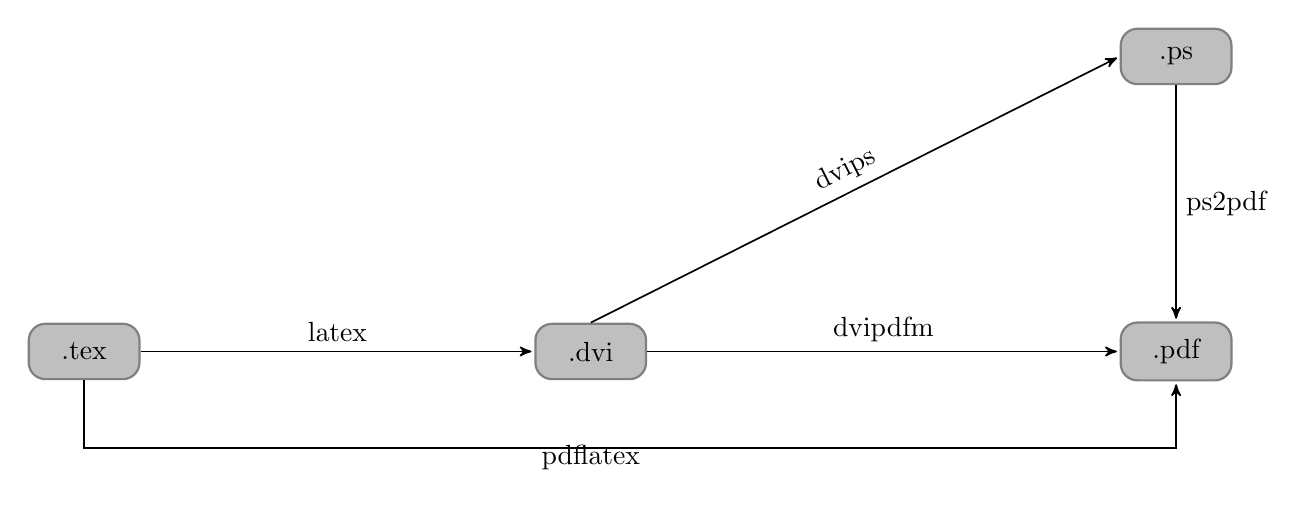
\begin{tikzpicture}
    \node[box] (tex) {.tex};
    \node[box] (dvi) [right=5 of tex] {.dvi};
    \node[box] (pdf) [right=6 of dvi] {.pdf};
    \node[box] (ps) [above=3 of pdf] {.ps};
    \path (tex) edge [arrow] node[auto] {latex} (dvi)
        (dvi) edge [arrow] node[auto] {dvipdfm} (pdf)
        (dvi.north) [arrow,draw] to node[above,sloped] {dvips} (ps.west)
        (ps) edge [arrow] node[right] {ps2pdf} (pdf)
        (tex) edge [arrow,bloop] (pdf);
    \node [below=.7 of dvi] {pdflatex};
\end{tikzpicture}
\caption{格式转换}
\label{fig:convert_format}
\end{figure}

最早的~driver~是~\verb|dvips|,它把~DVI~转换为~PS。\verb|dvipdf|~把~DVI~转为~PDF,它后来被~\verb|dvipdfm|~所取代;\verb|dvipdfm|~主要用于处理单字节字符,1999~年之后停止开发;在~\verb|dvipdfm|~基础上发展来的~\verb|dvipdfmx|~可以处理多字节编码(字符编码详见\ref{sec:encoding}节)。

pdf\TeX~是一种特殊的driver,它跳过~DVI,直接用~\TeX~源文件生成~PDF。基于~pdf\TeX~的~pdf\LaTeX~则把\LaTeX~源文件转为~PDF。

包老师倾向于~\verb|dvipdfmx|,因为它对图形格式的兼容性较好,而且擅长处理中文。

得到~DVI~后,我们可以在控制台用以下命令把它转为~PDF。
\begin{code}
dvipdfm hello_world(.dvi)
\end{code}

我们也可以把它转为~PS,接着用~Ghostscript~的一个命令行程序把它转换为~PDF,注意第二个命令需要~\verb|.ps|~后缀。一般情况下不推荐这种方法,因为它多了个步骤。
\begin{code}
dvips hello_world(.dvi)
ps2pdf hello_world.ps
\end{code}

pdf\LaTeX~用法如下。
\begin{code}
pdflatex hello_world(.tex)
\end{code}

\section{\LaTeX~语句}
\LaTeX~源文件的每一行称作一条语句(statement),语句可以分三种:命令(command)、数据(data)和注释(comment)。

命令分为两种:普通命令和环境(environment)。普通命令以\verb|\|~起始,大多只有一行;而环境包含一对起始声明和结尾声明,用于多行的场合。命令和环境可以互相嵌套。

数据就是普通内容。注释语句以~\verb|%|~起始,它在编译过程中被忽略。

例如在\ref{sec:hello_world}节例1中,第一行是注释,第二行是普通命令;第三、五行是环境的起始和结尾声明;第四行是数据。

\section{文档结构}
\subsection{文档类、序言、正文}
\LaTeX~源文件的结构分三大部分,依次为:文档类声明、序言(可选)、正文。

文档类声明用来指定文档的类型;序言(preamble)用来完成一些特殊任务,比如引入宏包,定义命令,设置环境等;文档的实际内容则放在正文部分。这里的正文指得是\verb|\begin{document}|和\verb|\end|~\verb|{document}|之间的部分,和通常人们心目中的“正文”概念有所出入。

这三部分的基本语法如下:
\begin{code}
\documentclass[options]{class}  %文档类声明
\usepackage[options]{package}   %引入宏包
...
\begin{document}                %正文
...
\end{document}
\end{code}

常用的文档类(documentclass)有三种:\verb|article、report、book|,它们的常用选项见\fref{tab:class_options}。

\begin{table}[htbp]
\centering
\caption{文档类常用选项}
\label{tab:class_options}
\begin{tabularx}{350pt}{lX}
    \toprule
    10pt, 11pt, 12pt & 正文字号,缺省10pt。\LaTeX~会根据正文字号选择标题、上下标等的字号。\\
    letterpaper, a4paper & 纸张尺寸,缺省是~letter。\\
    notitlepage, titlepage & 标题后是否另起新页。article~缺省~notitlepage,report~和~book~缺省有~titlepage。\\
    onecolumn, twocolumn & 栏数,缺省单栏。\\
    oneside, twoside & 单面双面。article~和~report~缺省单面,book~缺省双面。\\
    landscape & 打印方向横向,缺省纵向。\\
    openany, openright & 此选项只用于~report~和~book。report~缺省~openany~,book~缺省~openright。\\
    draft & 草稿模式。有时某些行排得过满,draft~模式可以在它们右边标上粗黑线提醒用户。\\
    \bottomrule
\end{tabularx}
\end{table}

\LaTeX~的核心只提供基本的功能,系统以宏包(package)的形式提供附加功能或增强原有功能。其它一些编程语言也有类似的模块化机制,比如~C/C++~的~\verb|#include|,Java~的~\verb|import|。

\subsection{标题、摘要、章节}


一份文档正文部分的开头通常有标题、作者、摘要等信息,之后是章节等层次结构,内容则散布于层次结构之间。

标题、作者、日期等命令如下,注意\verb|\maketitle|~命令要放在最后。
\begin{code}
\title{标题}
\author{作者}
\today
\maketitle
\end{code}

摘要环境用法如下:
\begin{code}
\begin{abstract}
...
\end{abstract}
\end{code}

常用的层次结构命令如下,
\begin{code}
\chapter{...}
\section{...}
\subsection{...}
\subsubsection{...}
\end{code}

每个高级层次可以包含若干低级层次。\verb|article|~中没有~\verb|chapter|,而~\verb|report|~和~\verb|book|~则支持上面所有层次。

\subsection{目录}

我们可以用~\verb|\tableofcontents|~命令来生成整个文档的目录,\LaTeX~会自动设定目录包含的章节层次,也可以用~\verb|\setcounter|~命令来指定目录层次深度。
\begin{code}
\tableofcontents
\setcounter{tocdepth}{2}
\end{code}

如果不想让某个章节标题出现在目录中,可以使用以下带~\verb|*|~的命令来声明章节。
\begin{code}
\chapter*{...}
\section*{...}
\subsection*{...}
\end{code}

类似地,我们也可以用以下命令生成插图和表格的目录,插图和表格功能将在后面章节中介绍。

\begin{code}
\listoffigures
\listoftables
\end{code}

当章节或图表等结构发生变化时,我们需要执行两遍编译命令以获得正确结果。\LaTeX~之所以设计成这样可能是因为当时的电脑内存容量有限。

\section{文字排版}
\subsection{字符输入}
文档中可以输入的内容大致可以分为:普通字符、控制符、特殊符号、注音符号、预定义字符串等。而这些内容有两种输入模式:文本模式(缺省)和数学模式,普通的行间(inline)数学模式用\verb|\$...\$|来表示。

\LaTeX~中有些字符(例如~\verb|# $ % ^ & _ { } ~ \|~等)被用作特殊的控制符,所以不能直接输入,多数需要在前面加个~\verb|\|。而~\verb|\|~本身则要用~\verb|\textbackslash|~命令来输入,因为~\verb|\\|~被用作了换行指令。很奇怪为什么不用~C~语言的~\verb|\n|,也许是因为~\TeX~的编程语言是~Pascal。

\begin{code}
\# \$ \% \^{} \& \_ \{ \} \~{} \textbackslash
\end{code}

\Fref{tab:symbol}~提供了一些符号的输入方法示例,完整的符号列表见~Scott Pakin的《The Comprehensive \LaTeX~ Symbol List》\citep{Pakin_2008}。

\begin{table}[htbp]
\centering
\caption{一些符号和预定义字符串}
\label{tab:symbol}
\begin{tabular}{llllll}
    \toprule
    \multicolumn{2}{c}{特殊符号} & \multicolumn{2}{c}{注音符号} & 
    \multicolumn{2}{c}{预定义字符串} \\
    \cmidrule(lr){1-2} \cmidrule(lr){3-4} \cmidrule(lr){5-6}
    \textcopyright  & \verb|\textcopyright|  & \aa & \verb|\aa| & 
        \today & \verb|\today| \\
    \textregistered & \verb|\textregistered| & \AA & \verb|\AA| & 
        \TeX & \verb|\TeX| \\
    $^\circ$C       & \verb|$^\circ$C|       & \ae & \verb|\ae| & 
        \LaTeX & \verb|\LaTeX| \\
    \textyen        & \verb|\textyen|        & \o  & \verb|\o| &
        \LaTeXe & \verb|\LaTeXe| \\
    \pounds         & \verb|\pounds|         & \"o & \verb|\"o| &
        \MF & \verb|\MF| \\
    \texteuro       & \verb|\texteuro|       & \^o & \verb|\^o| &
        \MP & \verb|\MP| \\
    \dots           & \verb|\dots|           & \~o & \verb|\~o| & \\
    \bottomrule
\end{tabular}
\end{table}

\subsection{换行、换页、断字}
通常~\LaTeX~会自动换行、换页。用户也可以用~\verb|\\|~或~\verb|\newline|~来强制换行;用~\verb|\newpage|~来强制换页。

一般情况下~\LaTeX~会尽量均匀地断字(Hyphenate),使得每一行的字间距分布整齐。但有时我们也需要显式指明断字位置,比如下例就指明~BASIC~这个词不能断开,而~blar-blar-blar~可以在-处断开。
\begin{code}
\hyphenation{BASIC blar-blar-blar}
\end{code}

\subsection{字样、字号}

\LaTeX~会自动调整正文、标题、章节、上下标、脚注等的字样\footnote{关于字样详见\ref{sec:typeface}节}、字号。我们也可以用\fref{tab:typeface_command}中的命令来设置字样;用\fref{tab:fontsize_command}中的命令来设置相对字号,比如正文字号是~10pt、11pt、12pt~时,tiny的字号就分别是~5pt、6pt、6pt。

\LaTeX~有一个特别的字样强调命令:\verb|\emph|,它在不同字样和装饰环境下有不同效果。比如周围文字是正体,它就是斜体;反之它就是正体。

\begin{table}[hbtp]
\centering
\caption{字样命令}
\label{tab:typeface_command}
\begin{tabular}{llll}
    \toprule
    \verb|\textrm{...}| & \textrm{roman} & 
    \verb|\textbf{...}| & \textbf{bold face} \\
    \verb|\textsf{...}| & \textsf{sans serif} & 
    \verb|\textit{...}| & \textit{italic} \\
    \verb|\texttt{...}| & \texttt{typewriter} & 
    \verb|\textsl{...}| & \textsl{slanted} \\
    \\
    \verb|\emph{...}|   & \emph{emphasized} & 
    \verb|\underline{...}|  & \underline{underline} \\
    \verb|\textsc{...}| & \textsc{Small Caps} & & \\
    \bottomrule
\end{tabular}
\end{table}

\begin{table}[htbp]
\centering
\caption{字号命令}
\label{tab:fontsize_command}
\begin{tabular}{llll}
    \toprule
    & \multicolumn{3}{c}{正文字号} \\
    \cmidrule(lr){2-4}
    命令 & 10pt & 11pt & 12pt \\
    \midrule
    \verb|\tiny|         & 5pt  & 6pt  & 6pt \\
    \verb|\scriptsize|   & 7pt  & 8pt  & 8pt \\
    \verb|\footnotesize| & 8pt  & 9pt  & 10pt \\
    \verb|\small|        & 9pt  & 10pt & 11pt \\
    \verb|\normalsize|   & 10pt & 11pt & 12pt \\
    \verb|\large|        & 12pt & 12pt & 14pt \\
    \verb|\Large|        & 14pt & 14pt & 17pt \\
    \verb|\LARGE|        & 17pt & 17pt & 20pt \\
    \verb|\huge|         & 20pt & 20pt & 25pt \\
    \verb|\Huge|         & 25pt & 25pt & 25pt \\
    \bottomrule
\end{tabular}
\end{table}

\section{常用命令环境}
\subsection{列表}

\LaTeX~中有三种列表环境:\verb|itemize、enumerate、description|,它们的一般用法如下:

\begin{demo}
\begin{itemize}
    \item C++
    \item Java
    \item HTML
\end{itemize}
\end{demo}

\begin{demo}
\begin{enumerate}
    \item C++
    \item Java
    \item HTML
\end{enumerate}
\end{demo}

\begin{demo}
\begin{description}
    \item{C++} 一种编程语言
    \item{Java} 另一种编程语言
    \item{HTML} 一种标记语言
\end{description}
\end{demo}

\subsection{对齐}
\LaTeX~中的段落缺省两端对齐(fully justified),我们也可以让段落居左、居右或居中对齐。

\begin{demo}
\begin{flushleft}
本段落\\
居左
\end{flushleft}
\end{demo}

\begin{demo}
\begin{flushright}
本段落\\
居右
\end{flushright}
\end{demo}

\begin{demo}
\begin{center}
本段落\\
居中
\end{center}
\end{demo}

\subsection{摘录}
\LaTeX~中有三种摘录环境:\verb|quote、quotation、verse|。\verb|quote|~两端都缩进,\verb|quotation|~在~\verb|quote|~的基础上增加了首行缩进,\verb|verse|~比~\verb|quote|~多了第二行起的缩进。

\begin{demo}
正文
\begin{quote}
引文两端都缩进。
\end{quote}
正文
\end{demo}

\begin{demo}
正文
\begin{quotation}
引文两端缩进,首行缩进。
\end{quotation}
正文
\end{demo}

\begin{demo}
正文
\begin{verse}
引文两端缩进,第二行起缩进。
\end{verse}
正文
\end{demo}

\subsection{原文照排}
一般文档中,命令和源代码通常使用等宽字样来表示,也就是原文照排。对此~\LaTeX~提供了~\verb|\verb|~命令(一般用于在正文中插入较短的命令)和~\verb|verbatim|~环境。后者有带~\verb|*|~的版本用来标明空格。

\begin{demo}
正文中插入\verb|command|
\begin{verbatim}
printf("Hello, world!");
\end{verbatim}
\begin{verbatim*}
printf("Hello, world!");
\end{verbatim*}
\end{demo}

\subsection{交叉引用}
我们常常需要引用文档中~\verb|section、subsection、figure、table|~等对象的编号,这种功能叫作交叉引用(cross referencing)。

\LaTeX~中可以用~\verb|\label{marker}|~命令来定义一个标记,标记名可以是任意字符串,但是在全文中须保持唯一。之后可以用~\verb|\ref{marker}|~命令来引用标记处章节或图表的编号,用~\verb|\pageref{marker}|~来引用标记处的页码。

\begin{demo}
被引用处\label{sec}\\
...\\
第\pageref{sec}页\ref{sec}节
\end{demo}

文档中新增交叉引用后,第一次执行~\verb|latex|~或~\verb|pdflatex|~编译命令时会得到类似下面的警告信息。因为第一次编译只会扫描出有交叉引用的地方,第二次编译才能得到正确结果。

\begin{code}
LaTeX Warning: There were undefined references.
...
LaTeX Warning: Label(s) may have changed. Rerun to get cross-
references right.
\end{code}

\subsection{脚注}
脚注(footnote)的一般用法如下:
\begin{demo}
这里是一段正文。\footnote{这里是一段脚注。}
\end{demo}

\section{长度单位}
\LaTeX~中的常用长度单位如\Fref{tab:unit}~所示。point~是个传统印刷业采用的单位,而~big point~是~Adobe~推出~PS~时新定义的单位。em~是个相对单位,比如当前字体是~11pt~时,1em~就是~11pt。
\begin{table}[htbp]
\caption{常用长度单位}
\label{tab:unit}
\centering
\begin{tabular}{llllll}
    \toprule
    in & 英寸 & pt & point, 1/72.27 in  & em & 当前字体中字母M的宽度 \\
    cm & 厘米 & bp & big point, 1/72 in & ex & 当前字体中字母x的高度 \\
    mm & 毫米 & pc & pica, 12 pt        & mu & math unit,1/18 em \\
    \bottomrule
\end{tabular}
\end{table}

\section{盒子}
\LaTeX~在排版时把每个对象(小到一个字母,大到一个段落)都视为一个矩形盒子(box),我们在~HTML~和~CSS~中也可以见到类似的模型。

\subsection{mbox~和~fbox}

\LaTeX~中最简单的盒子是~\verb|\mbox|~和~\verb|\fbox|。前者把一组对象组合起来,后者在此基础上加了个边框。
\begin{demo}
\mbox{010 6278 5001}
\fbox{010 6278 5001}
\end{demo}

\subsection{makebox~和~framebox}
稍复杂的~\verb|\makebox|~和~\verb|\framebox|~提供了宽度和对齐方式控制选项。这里用~l、r、s~分别代表居左、居右和分散对齐。
\begin{demo}
%语法:[宽度][对齐方式]{内容}
\makebox[100pt][l]{居左}
\framebox[100pt][r]{居右}
\end{demo}

\subsection{parbox~和~minipage}
大一些的对象比如整个段落可以用~\verb|\parbox|~命令和~\verb|\minipage|~环境,两者语法类似,也提供了对齐方式和宽度的选项。但是这里的对齐方式是指与周围内容的纵向关系,用~t、c、b~分别代表居顶、居中和居底对齐。

\begin{demo}
%语法:[对齐方式]{宽度}{内容}
\parbox[c]{90pt}{锦瑟无端五十弦,\\一弦一柱思华年。}李商隐
\end{demo}

细心的读者会发现~\verb|\parbox|~和~\verb|\minipage|~的选项排列顺序和~\verb|\makebox|~和~\verb~\framebox|~的不一致,可能出自不同的作者。

\bibliographystyle{unsrtnat}
\bibliography{reading}
\newpage

% -*- coding: utf-8 -*-
% This is part of the book TeX for the Impatient.
% Copyright (C) 2003 Paul W. Abrahams, Kathryn A. Hargreaves, Karl Berry.
% See file fdl.tex for copying conditions.

\input macros
\chapter {数学公式命令}

\bix^^{math}
\chapterdef{math}

这一章包括了排印数学公式所需要的命令。
在\headcit{命令描述}{cmddesc}这一节中给出了这章的惯例。

\begindescriptions
%==========================================================================
\section {简单公式排版}

%==========================================================================
\subsection {希腊字母}

\begindesc
\bix^^{Greek letters}
\dothreecolumns 40
\easy\ctsdisplay alpha {}
\ctsdisplay beta {}
\ctsdisplay chi {}
\ctsdisplay delta {}
\ctsdisplay Delta {}
\ctsdisplay epsilon {}
\ctsdisplay varepsilon {}
\ctsdisplay eta {}
\ctsdisplay gamma {}
\ctsdisplay Gamma {}
\ctsdisplay iota {}
\ctsdisplay kappa {}
\ctsdisplay lambda {}
\ctsdisplay Lambda {}
\ctsdisplay mu {}
\ctsdisplay nu {}
\ctsdisplay omega {}
\ctsdisplay Omega {}
\ctsdisplay phi {}
\ctsdisplay varphi {}
\ctsdisplay Phi {}
\ctsdisplay pi {}
\ctsdisplay varpi {}
\ctsdisplay Pi {}
\ctsdisplay psi {}
\ctsdisplay Psi {}
\ctsdisplay rho {}
\ctsdisplay varrho {}
\ctsdisplay sigma {}
\ctsdisplay varsigma {}
\ctsdisplay Sigma {}
\ctsdisplay tau {}
\ctsdisplay theta {}
\ctsdisplay vartheta {}
\ctsdisplay Theta {}
\ctsdisplay upsilon {}
\ctsdisplay Upsilon {}
\ctsdisplay xi {}
\ctsdisplay Xi {}
\ctsdisplay zeta {}
\egroup
\explain
输入这些命令可以排印出数学公式中的相应的希腊字母符号.
你只能在数学模式中使用它们, 所以如在普通的文本中使用它们时,
你必须把它们括在美元符号 (|$|) 内.
\TeX\ 并不包含这些数学中使用的希腊字母所对应的正体字符的命令,
不过你可以很方便地得到这些字符.
比如说, 你可以在公式中使用 `|{\rm o}|' 来得到一个小写的 ^{omicron} `o',
又比如, 你可以使用 `|{\rm B}|' 得到大写的 beta (`B').

注意不要混淆下面的符号:
\ulist \compact
\li |\upsilon| (`$\upsilon$'), |{\rm v}| (`v'), 和 |\nu| (`$\nu$').
\li |\varsigma| (`$\varsigma$') 和 |\zeta| (`$\zeta$').
\endulist

使用数学的意大利\minref{字体} (|\mit|) 可以得到斜体的大写希腊字母.

在计算在希腊字母周围插入多少的空白时, \TeX\ 把它们当作正常的符号.

\example
如果 $\rho$ 和 $\theta$ 都是正数, 那么 $f(\theta)
-{\mit \Gamma}_{\theta} < f(\rho)-{\mit \Gamma}_{\rho}$.
|
\produces
如果 $\rho$ 和 $\theta$ 都是正数, 那么
$f(\theta)-{\mit \Gamma}_{\theta} < f(\rho)-{\mit \Gamma}_{\rho}$.
\endexample
\eix^^{Greek letters}
\enddesc

%==========================================================================
%\subsection {Miscellaneous ordinary math symbols}
\subsection {各种普通数学符号}

\begindesc
\xrdef{specsyms}
\dothreecolumns 34
\easy\ctsdisplay infty {}
\ctsdisplay Re {}
\ctsdisplay Im {}
\ctsdisplay angle {}
\ctsdisplay triangle {}
\ctsdisplay backslash {}
\ctsdisplay vert {}
\ctsydisplay | @bar {}
\ctsdisplay Vert {}
\ctsdisplay emptyset {}
\ctsdisplay bot {}
\ctsdisplay top {}
\ctsdisplay exists {}
\ctsdisplay forall {}
\ctsdisplay hbar {}
\ctsdisplay ell {}
\ctsdisplay aleph {}
\ctsdisplay imath {}
\ctsdisplay jmath {}
\ctsdisplay nabla {}
\ctsdisplay neg {}
\ctsdisplay lnot {}
\actdisplay ' @prime \ (上标点)
\ctsdisplay prime {}
\ctsdisplay partial {}
\ctsdisplay surd {}
\ctsdisplay wp {}
\ctsdisplay flat {}
\ctsdisplay sharp {}
\ctsdisplay natural {}
\ctsdisplay clubsuit {}
\ctsdisplay diamondsuit {}
\ctsdisplay heartsuit {}
\ctsdisplay spadesuit {}
\egroup
\explain
^^{music symbols} ^^{card suits}
这些命令可以排印各种符号.
为了把它们和其它的符号, 比如关系符号等, 区分开来, 它们被称为普通数学符号.
你只能在数学模式中使用这些符号, 所以如果在普通的文本中使用, 你必须使用美元符号 (|$|) 把它们括起来.

当你想在 `$i$' 或 `$j$' 上加上重音符号, 则需要使用 |\imath| 和 |\jmath| 命令来表示它们本身.

上标点符号 (|'|) 是一个 |\prime| 的上标的简写.
(|\prime| 本身可以排印一个很大的丑陋的撇号.)

|\!|| 和 ^|\Vert| 命令是等价的, 就像 ^|\neg| 和 ^|\lnot| 命令一样.
\margin{增加了 {\tt\\vert} 的解释}
|\vert| 符号可以排印出和 `|!||' 相同的效果.
\indexchar |

由 |\backslash|, |\vert|, 和 |\Vert| 排印的命令叫做 \minref{分界符}.
使用 ^|\bigm| 等 (\xref \bigm) 命令可以排印大号的这些字符.

\example
The Knave of $\heartsuit$s, he stole some tarts.
|
\produces
The Knave of $\heartsuit$s, he stole some tarts.
\nextexample
如 $\hat\imath < \hat\jmath$ 则 $i' \leq j^\prime$.
|
\produces
如 $\hat\imath < \hat\jmath$ 则 $i' \leq j^\prime$.
\nextexample
$${{x-a}\over{x+a}}\biggm\backslash{{y-b}\over{y+b}}$$
|
\dproduces
$${{x-a}\over{x+a}}\biggm\backslash{{y-b}\over{y+b}}$$
\endexample
\enddesc

%==========================================================================
\subsection {二元运算符}

\begindesc
\bix^^{operations}
\xrdef{binops}
\dothreecolumns 34
\easy\ctsdisplay vee {}
\ctsdisplay wedge {}
\ctsdisplay amalg {}
\ctsdisplay cap {}
\ctsdisplay cup {}
\ctsdisplay uplus {}
\ctsdisplay sqcap {}
\ctsdisplay sqcup {}
\ctsdisplay dagger {}
\ctsdisplay ddagger {}
\ctsdisplay land {}
\ctsdisplay lor {}
\ctsdisplay cdot {}
\ctsdisplay diamond {}
\ctsdisplay bullet {}
\ctsdisplay circ {}
\ctsdisplay bigcirc {}
\ctsdisplay odot {}
\ctsdisplay ominus {}
\ctsdisplay oplus {}
\ctsdisplay oslash {}
\ctsdisplay otimes {}
\ctsdisplay pm {}
\ctsdisplay mp {}
\ctsdisplay triangleleft {}
\ctsdisplay triangleright {}
\ctsdisplay bigtriangledown {}
\ctsdisplay bigtriangleup {}
\ctsdisplay ast {}
\ctsdisplay star {}
\ctsdisplay times {}
\ctsdisplay div {}
\ctsdisplay setminus {}
\ctsdisplay wr {}
\egroup
\explain
这些命令可以排印各种二元运算符.
二元运算符是 \TeX\ 的一种符号\minref{集}.
\TeX\ 在不同的符号集周围会插入不同的空白.
当 \TeX\ 需要在一个数学公式中间断行时,
它会考虑在二元运算符后面进行断行---不过仅在它出现在公式的最外层时, 而不是在一个组中.

除了这些命令以外, \TeX\ 也把 `|+|' and `|-|' 作为二元运算符.
它把 `|/|' 当作一个普通符号,
因为虽然事实上在数学中它是一个二元运算,
但是它在周围加入的空白更少时看上去更漂亮.

\example
$$z = x \div y \quad \hbox{当且仅当} \quad
z \times y = x \;\hbox{且}\; y \neq 0$$
|
\dproduces
$$z = x \div y \quad \hbox{当且仅当} \quad
z \times y = x \;\hbox{且}\; y \neq 0$$
\endexample
\enddesc

\begindesc
\ctspecial * \ctsxrdef{@star}
\explain
命令 |\*| 表示乘法符号 ($\times$), 也是一个二元符号.
乘法符号在文本中的数学公式中出现时表现得和一个分词符类似.
这就是说, \TeX\ \emph{仅}会在公式该点需要断行时排版 |\times| 符号.
因为 \TeX\ 永远不会在陈列公式中断行, 所以 |\*| 在陈列公式 \minrefs{陈列公式} 中是没有任何作用的.

\example
Let $c = a\*b$. In the case that $c=0$ or $c=1$, let
$\Delta$ be $(\hbox{the smallest $q$})\*(\hbox{the
largest $q$})$ in the set of approximate $\tau$-values.
|
\produces
Let $c = a\*b$. In the case that $c=0$ or $c=1$, let
$\Delta$ be $(\hbox{the smallest $q$})\*(\hbox{the
largest $q$})$ in the set of approximate $\tau$-values.

\eix^^{operations}
\endexample
\enddesc

%==========================================================================
\subsection {关系符号}

\begindesc
\xrdef {relations}
\bix^^{relations}
\dothreecolumns 39
\easy\ctsdisplay asymp {}
\ctsdisplay cong {}
\ctsdisplay dashv {}
\ctsdisplay vdash {}
\ctsdisplay perp {}
\ctsdisplay mid {}
\ctsdisplay parallel {}
\ctsdisplay doteq {}
\ctsdisplay equiv {}
\ctsdisplay ge {}
\ctsdisplay geq {}
\ctsdisplay le {}
\ctsdisplay leq {}
\ctsdisplay gg {}
\ctsdisplay ll {}
\ctsdisplay models {}
\ctsdisplay ne {}
\ctsdisplay neq {}
\ctsdisplay notin {}
\ctsdisplay in {}
\ctsdisplay ni {}
\ctsdisplay owns {}
\ctsdisplay prec {}
\ctsdisplay preceq {}
\ctsdisplay succ {}
\ctsdisplay succeq {}
\ctsdisplay bowtie {}
\ctsdisplay propto {}
\ctsdisplay approx {}
\ctsdisplay sim {}
\ctsdisplay simeq {}
\ctsdisplay frown {}
\ctsdisplay smile {}
\ctsdisplay subset {}
\ctsdisplay subseteq {}
\ctsdisplay supset {}
\ctsdisplay supseteq {}
\ctsdisplay sqsubseteq {}
\ctsdisplay sqsupseteq {}
\egroup
\explain
这些命令可以排印各种关系符号.
关系符号是 \TeX\ 的数学符号中的\minref{类}之一.
\TeX\ 在不同的\minref{类}之间插入不同的空白长度.
当 \TeX\ 需要在一个数学公式处断行, \minrefs{断行}
它会考虑在一个关系符后进行断行---不过仅在它出现在公式的最外层时, 而不是在一个组中.

除了这里列出的命令以外, \TeX\ 也把 `^|=|' 和``arrow'' 命令 (\xref{arrows}) 作为关系运算符.

一些关系符有多种命令表达方式, 你可以使用任何一个来排印它们:
\ulist \compact
\li `$\ge$' (|\ge| 和 |\geq|).
\li `$\le$' (|\le| 和 |\leq|).
\li `$\ne$' (|\ne|, |\neq|, 和 |\not=|).
\li `$\ni$' (|\ni| 和 |\owns|).
\endulist

\xrdef{\not}
在这些符号前加上 |\not|, 可以排印它们的非运算:

\nobreak
\threecolumns 21
\basicdisplay {$\not\asymp$}{\\not\\asymp}\ctsidxref{asymp}
\basicdisplay {$\not\cong$}{\\not\\cong}\ctsidxref{cong}
\basicdisplay {$\not\equiv$}{\\not\\equiv}\ctsidxref{equiv}
\basicdisplay {$\not=$}{\\not=}\ttidxref{=}
\basicdisplay {$\not\ge$}{\\not\\ge}\ctsidxref{ge}
\basicdisplay {$\not\geq$}{\\not\\geq}\ctsidxref{geq}
\basicdisplay {$\not\le$}{\\not\\le}\ctsidxref{le}
\basicdisplay {$\not\leq$}{\\not\\leq}\ctsidxref{leq}
\basicdisplay {$\not\prec$}{\\not\\prec}\ctsidxref{prec}
\basicdisplay {$\not\preceq$}{\\not\\preceq}\ctsidxref{preceq}
\basicdisplay {$\not\succ$}{\\not\\succ}\ctsidxref{succ}
\basicdisplay {$\not\succeq$}{\\not\\succeq}\ctsidxref{succeq}
\basicdisplay {$\not\approx$}{\\not\\approx}\ctsidxref{approx}
\basicdisplay {$\not\sim$}{\\not\\sim}\ctsidxref{sim}
\basicdisplay {$\not\simeq$}{\\not\\simeq}\ctsidxref{simeq}
\basicdisplay {$\not\subset$}{\\not\\subset}\ctsidxref{subset}
\basicdisplay {$\not\subseteq$}{\\not\\subseteq}\ctsidxref{subseteq}
\basicdisplay {$\not\supset$}{\\not\\supset}\ctsidxref{supset}
\basicdisplay {$\not\supseteq$}{\\not\\supseteq}\ctsidxref{supseteq}
\basicdisplay {$\not\sqsubseteq$}{\\not\\sqsubseteq}%
   \ctsidxref{sqsubseteq}
\basicdisplay {$\not\sqsupseteq$}{\\not\\sqsupseteq}%
   \ctsidxref{sqsupseteq}
\egroup

\example
我们可以得到 $AB \perp AC$,且
$\triangle ABF \not\sim \triangle ACF$.
|
\produces
我们可以得到 $AB \perp AC$,且
$\triangle ABF \not\sim \triangle ACF$.

\eix^^{relations}
\endexample
\enddesc

%==========================================================================
%\subsection {Left and right delimiters}
\subsection {左右定界符}

%\begindesc
%\bix^^{delimiters}
%%
%\dothreecolumns 12
%\easy\ctsdisplay lbrace {}
%\ctsydisplay { @lbrace {}
%\ctsdisplay rbrace {}
%\ctsydisplay } @rbrace {}
%\ctsdisplay lbrack {}
%\ctsdisplay rbrack {}
%\ctsdisplay langle {}
%\ctsdisplay rangle {}
%\ctsdisplay lceil {}
%\ctsdisplay rceil {}
%\ctsdisplay lfloor {}
%\ctsdisplay rfloor {}
%\egroup
%\explain
%These commands produce left and right \minref{delimiter}s.
%Mathematicians use delimiters to indicate the boundaries between parts
%of a formula.  Left delimiters are also called ``^{opening}s'', and
%right delimiters are also called ``^{closing}s''.  Openings and closings
%are two of \TeX's \minref{class}es of math symbols.  \TeX\ puts
%different amounts of space around different \minref{class}es of math
%symbols. You might expect the space that \TeX\ puts around openings and
%closings to be symmetrical, but in fact it isn't.
\begindesc
\bix^^{delimiters}
%
\dothreecolumns 12
\easy\ctsdisplay lbrace {}
\ctsydisplay { @lbrace {}
\ctsdisplay rbrace {}
\ctsydisplay } @rbrace {}
\ctsdisplay lbrack {}
\ctsdisplay rbrack {}
\ctsdisplay langle {}
\ctsdisplay rangle {}
\ctsdisplay lceil {}
\ctsdisplay rceil {}
\ctsdisplay lfloor {}
\ctsdisplay rfloor {}
\egroup
\explain
这些命令排印各种左右\minref{定界符}。
数学家用定界符指明公式各部分的边界。
左定界符又称为``^{开符号}'',右定界符又称为``^{闭符号}''。
开符号和闭符号是 \TeX\ 数学公式中的两种字符类。
\TeX\ 在不同\minref{类}的数学符号之间留下不同大小的间隔。
你也许认为在开符号和闭符号旁边的间隔是对称的,但实际上并非如此。

%Some left and right delimiters have more than one command that you can
%use to produce them:
有些左定界符和右定界符可以用不止一个命令排印:

%\ulist\compact
%\li `$\{$' (|\lbrace| and |\{|)
%\li `$\}$' (|\rbrace| and |\}|)
%\li `$[$' (|\lbrack| and `|[|')
%\li `$]$' (|\rbrack| and `|]|')
%\endulist
%\noindent You can also use the left and right bracket characters
%(in either form) outside of math mode.
\ulist\compact
\li `$\{$' (|\lbrace| 和 |\{|)
\li `$\}$' (|\rbrace| 和 |\}|)
\li `$[$' (|\lbrack| 和 `|[|')
\li `$]$' (|\rbrack| 和 `|]|')
\endulist
\noindent 左右方括号(两种形式皆可)在数学模式之外也可以使用。

%In addition to these commands, \TeX\ treats `|(|' as a left
%delimiter and `|)|' as a right delimiter.
除这些命令之外,\TeX\ 还将 `|(|' 视为左定界符,将 `|)|' 视为右定界符。

%You can have \TeX\
%choose the size for a delimiter by using |\left| and |\right| (\xref\left).
%Alternatively,
%you can get a delimiter of a specific size by using one of the |\big|$x$
%commands (see |\big| et al., \xref{\big}).
利用 |\left| 和 |\right|(\xref\left )命令,
你可以让 \TeX\ 选择定界符的尺寸。
或者利用某个 |\big|$x$ 命令(见 |\big| 等,\xref{\big}),
你可以选择特定尺寸的定界符。

%\example
%The set $\{\,x \mid x>0\,\}$ is empty.
%|
%\produces
%The set $\{\,x \mid x>0\,\}$ is empty.
\example
集合 $\{\,x \mid x>0\,\}$ 是空集.
|
\produces
集合 $\{\,x \mid x>0\,\}$ 是空集.

%\eix^^{delimiters}
%\endexample
%\enddesc
\eix^^{delimiters}
\endexample
\enddesc

%==========================================================================
%\subsection {Arrows}
\subsection {箭头}

%\begindesc
%\bix^^{arrows}
%\xrdef{arrows}
%%
%{\symbolspace=24pt \makecolumns 34/2:
%\easy%
%\ctsdisplay leftarrow {}
%\ctsdisplay gets {}
%\ctsdisplay Leftarrow {}
%\ctsdisplay rightarrow {}
%\ctsdisplay to {}
%\ctsdisplay Rightarrow {}
%\ctsdisplay leftrightarrow {}
%\ctsdisplay Leftrightarrow {}
%\ctsdisplay longleftarrow {}
%\ctsdisplay Longleftarrow {}
%\ctsdisplay longrightarrow {}
%\ctsdisplay Longrightarrow {}
%\ctsdisplay longleftrightarrow {}
%\ctsdisplay Longleftrightarrow {}
%\basicdisplay {$\Longleftrightarrow$}{\\iff}\pix\ctsidxref{iff}\xrdef{\iff}
%\ctsdisplay hookleftarrow {}
%\ctsdisplay hookrightarrow {}
%\ctsdisplay leftharpoondown {}
%\ctsdisplay rightharpoondown {}
%\ctsdisplay leftharpoonup {}
%\ctsdisplay rightharpoonup {}
%\ctsdisplay rightleftharpoons {}
%\ctsdisplay mapsto {}
%\ctsdisplay longmapsto {}
%\ctsdisplay downarrow {}
%\ctsdisplay Downarrow {}
%\ctsdisplay uparrow {}
%\ctsdisplay Uparrow {}
%\ctsdisplay updownarrow {}
%\ctsdisplay Updownarrow {}
%\ctsdisplay nearrow {}
%\ctsdisplay searrow {}
%\ctsdisplay nwarrow {}
%\ctsdisplay swarrow {}
%}
%\explain
%These commands provide arrows of different kinds.  They
%are classified as relations (\xref{relations}).
%The vertical arrows in the list are also \minref{delimiter}s, so you can make
%them larger by using |\big| et al.\ (\xref \big).
\begindesc
\bix^^{arrows}
\xrdef{arrows}
%
{\symbolspace=24pt \makecolumns 34/2:
\easy%
\ctsdisplay leftarrow {}
\ctsdisplay gets {}
\ctsdisplay Leftarrow {}
\ctsdisplay rightarrow {}
\ctsdisplay to {}
\ctsdisplay Rightarrow {}
\ctsdisplay leftrightarrow {}
\ctsdisplay Leftrightarrow {}
\ctsdisplay longleftarrow {}
\ctsdisplay Longleftarrow {}
\ctsdisplay longrightarrow {}
\ctsdisplay Longrightarrow {}
\ctsdisplay longleftrightarrow {}
\ctsdisplay Longleftrightarrow {}
\basicdisplay {$\Longleftrightarrow$}{\\iff}\pix\ctsidxref{iff}\xrdef{\iff}
\ctsdisplay hookleftarrow {}
\ctsdisplay hookrightarrow {}
\ctsdisplay leftharpoondown {}
\ctsdisplay rightharpoondown {}
\ctsdisplay leftharpoonup {}
\ctsdisplay rightharpoonup {}
\ctsdisplay rightleftharpoons {}
\ctsdisplay mapsto {}
\ctsdisplay longmapsto {}
\ctsdisplay downarrow {}
\ctsdisplay Downarrow {}
\ctsdisplay uparrow {}
\ctsdisplay Uparrow {}
\ctsdisplay updownarrow {}
\ctsdisplay Updownarrow {}
\ctsdisplay nearrow {}
\ctsdisplay searrow {}
\ctsdisplay nwarrow {}
\ctsdisplay swarrow {}
}
\explain
这些命令提供各种箭头。它们被划分为关系符号(\xref{relations})。
上面的竖直箭头同时也是\minref{定界符},
因此你可以用 |\big| 等命令让它们变大(\xref \big )。

%The command |\iff| differs from |\Longleftrightarrow| in that
%it produces extra space to the left and right of the arrow.
命令 |\iff| 和 |\Longleftrightarrow| 的差别之处在于,
它在箭头两边生成额外间隔。

%You can place symbols or other legends on top of a left or right arrow
%with |\buildrel| (\xref \buildrel).
你可以用 |\buildrel|(\xref \buildrel )命令将符号或者其他文字放在箭头上边。

%\example
%$$f(x)\mapsto f(y) \iff x \mapsto y$$
%|
%\dproduces
%$$f(x)\mapsto f(y) \iff x \mapsto y$$
\example
$$f(x)\mapsto f(y) \iff x \mapsto y$$
|
\dproduces
$$f(x)\mapsto f(y) \iff x \mapsto y$$

%\eix^^{arrows}
%\endexample
%\enddesc
\eix^^{arrows}
\endexample
\enddesc

%==========================================================================
%\subsection {Named mathematical functions}
\subsection {已命名的数学函数}

%\begindesc
%\xrdef{namedfns}
%\bix^^{functions, names of}
%{\symbolspace = 36pt
%\threecolumns 32
%\easy\ctsdisplay cos {}
%\ctsdisplay sin {}
%\ctsdisplay tan {}
%\ctsdisplay cot {}
%\ctsdisplay csc {}
%\ctsdisplay sec {}
%\ctsdisplay arccos {}
%\ctsdisplay arcsin {}
%\ctsdisplay arctan {}
%\ctsdisplay cosh {}
%\ctsdisplay coth {}
%\ctsdisplay sinh {}
%\ctsdisplay tanh {}
%\ctsdisplay det {}
%\ctsdisplay dim {}
%\ctsdisplay exp {}
%\ctsdisplay ln {}
%\ctsdisplay log {}
%\ctsdisplay lg {}
%\ctsdisplay arg {}
%\ctsdisplay deg {}
%\ctsdisplay gcd {}
%\ctsdisplay hom {}
%\ctsdisplay ker {}
%\ctsdisplay inf {}
%\ctsdisplay sup {}
%\ctsdisplay lim {}
%\ctsdisplay liminf {}
%\ctsdisplay limsup {}
%\ctsdisplay max {}
%\ctsdisplay min {}
%\ctsdisplay Pr {}
%\egroup}
%\explain
%These commands set the names of various mathematical functions
%in roman type, as is customary.
%If you apply a superscript or subscript to one of these commands,
%\TeX\ will in most cases typeset it in the usual place.
%In display style, \TeX\ typesets superscripts and subscripts
%on |\det|, |\gcd|, |\inf|, |\lim|, |\liminf|,
%|\limsup|, |\max|, |\min|, |\Pr|, and |\sup|
%as though they were limits,
%i.e., directly above or directly below the function name.
\begindesc
\xrdef{namedfns}
\bix^^{functions, names of}
{\symbolspace = 36pt
\threecolumns 32
\easy\ctsdisplay cos {}
\ctsdisplay sin {}
\ctsdisplay tan {}
\ctsdisplay cot {}
\ctsdisplay csc {}
\ctsdisplay sec {}
\ctsdisplay arccos {}
\ctsdisplay arcsin {}
\ctsdisplay arctan {}
\ctsdisplay cosh {}
\ctsdisplay coth {}
\ctsdisplay sinh {}
\ctsdisplay tanh {}
\ctsdisplay det {}
\ctsdisplay dim {}
\ctsdisplay exp {}
\ctsdisplay ln {}
\ctsdisplay log {}
\ctsdisplay lg {}
\ctsdisplay arg {}
\ctsdisplay deg {}
\ctsdisplay gcd {}
\ctsdisplay hom {}
\ctsdisplay ker {}
\ctsdisplay inf {}
\ctsdisplay sup {}
\ctsdisplay lim {}
\ctsdisplay liminf {}
\ctsdisplay limsup {}
\ctsdisplay max {}
\ctsdisplay min {}
\ctsdisplay Pr {}
\egroup}
\explain
这些命令以惯用的罗马字体排印各种数学函数的名称。
如果你给这些命令中的任何一个加上上标或下标,
\TeX\ 将在通常的位置排版它。
在陈列样式中,对于 |\det|、|\gcd|、|\inf|、|\lim|、|\liminf|、
|\limsup|、|\max|、|\min|、|\Pr| 和 |\sup|,
\TeX\ 将上标和下标当成极限那样排版,
即将它们直接放在函数名的上边或下边。

%\example
%$\cos^2 x + \sin^2 x = 1\qquad\max_{a \in A} g(a) = 1$
%|
%\produces
%$\cos^2 x + \sin^2 x = 1\qquad\max_{a \in A} g(a) = 1$
%\endexample\enddesc
\example
$\cos^2 x + \sin^2 x = 1\qquad\max_{a \in A} g(a) = 1$
|
\produces
$\cos^2 x + \sin^2 x = 1\qquad\max_{a \in A} g(a) = 1$
\endexample\enddesc

%\begindesc
%\cts bmod {}
%\explain
%This command produces a binary operation for indicating a ^{modulus}
%within a formula.
%\example
%$$x = (y+1) \bmod 2$$
%|
%\dproduces
%$$x = (y+1) \bmod 2$$
%\endexample
%\enddesc
\begindesc
\cts bmod {}
\explain
此命令排印一个标明公式内的^{模运算}的二元运算符。
\example
$$x = (y+1) \bmod 2$$
|
\dproduces
$$x = (y+1) \bmod 2$$
\endexample
\enddesc

%\begindesc
%\cts pmod {}
%\explain
%This command provides a notation for indicating a ^{modulus} in parentheses
%at the end of a formula.
%\example
%$$x \equiv y+1 \pmod 2$$
%|
%\dproduces
%$$x \equiv y+1 \pmod 2$$
\begindesc
\cts pmod {}
\explain
此命令在公式末尾排印放在圆括号中的^{模运算}。
\example
$$x \equiv y+1 \pmod 2$$
|
\dproduces
$$x \equiv y+1 \pmod 2$$

%\eix^^{functions, names of}
%\endexample
%\enddesc
\eix^^{functions, names of}
\endexample
\enddesc


%==========================================================================
%\subsection {Large operators}
\subsection {巨算符}

%\begindesc
%\bix^^{operators//large}
%\threecolumns 15
%\easy\ctsdoubledisplay bigcap {}
%\ctsdoubledisplay bigcup {}
%\ctsdoubledisplay bigodot {}
%\ctsdoubledisplay bigoplus {}
%\ctsdoubledisplay bigotimes {}
%\ctsdoubledisplay bigsqcup {}
%\ctsdoubledisplay biguplus {}
%\ctsdoubledisplay bigvee {}
%\ctsdoubledisplay bigwedge {}
%\ctsdoubledisplay coprod {}
%{\symbolspace = 42pt\basicdisplay {\hskip 26pt$\smallint$}%
%   {\\smallint}\ddstrut}%
%   \xrdef{\smallint} \pix\ctsidxref{smallint}
%\ctsdoubledisplay int {}
%\ctsdoubledisplay oint {}
%\ctsdoubledisplay prod {}
%\ctsdoubledisplay sum {}
%}
%\explain
%These commands produce various large operator symbols.
%\TeX\ produces the smaller size when it's in ^{text style}
%\minrefs{math mode} and the larger size when it's in ^{display style}.
%Operators are one of \TeX's \minref{class}es of math symbols.
%\TeX\ puts different amounts of space
%around different classes of math symbols.
\begindesc
\bix^^{operators//large}
\threecolumns 15
\easy\ctsdoubledisplay bigcap {}
\ctsdoubledisplay bigcup {}
\ctsdoubledisplay bigodot {}
\ctsdoubledisplay bigoplus {}
\ctsdoubledisplay bigotimes {}
\ctsdoubledisplay bigsqcup {}
\ctsdoubledisplay biguplus {}
\ctsdoubledisplay bigvee {}
\ctsdoubledisplay bigwedge {}
\ctsdoubledisplay coprod {}
{\symbolspace = 42pt\basicdisplay {\hskip 26pt$\smallint$}%
   {\\smallint}\ddstrut}%
   \xrdef{\smallint} \pix\ctsidxref{smallint}
\ctsdoubledisplay int {}
\ctsdoubledisplay oint {}
\ctsdoubledisplay prod {}
\ctsdoubledisplay sum {}
}
\explain
这些命令排印各种巨算符。
\TeX\ 在^{文内样式}中排印小号字符,
\minrefs{math mode}而在^{陈列样式}中排印大号字符.
巨算符是 \TeX\ 数学符号的其中一\minref{类}。
\TeX\ 在不同类数学符号间留下不同大小的间隔。

%The large operator symbols with `|big|' in their names are different
%from the corresponding binary operations (see \xref{binops}) such as
%|\cap| ($\cap$) since they usually appear at the beginning
%of a formula.  \TeX\ uses different spacing for a large operator
%than it does for a binary operation.
名称中带有 `|big|' 的巨算符和对应的二元运算符%
(比如 |\cap| ($\cap$),见\xref{binops})不同,
因为它们通常出现公式的开头。
\TeX\ 给巨算符留下的间隔与二元运算符的不同。

%Don't confuse `$\sum$' (|\sum|) with `$\Sigma$'^^|\Sigma| (|\Sigma|)
%or confuse `$\prod$' (|\prod|) with `$\Pi$' ^^|\Pi| (|\Pi|).
%|\Sigma| and |\Pi| produce capital Greek letters, which are smaller and
%have a different appearance.
不要混淆 `$\sum$' (|\sum|) 和 `$\Sigma$'^^|\Sigma| (|\Sigma|),
或者 `$\prod$' (|\prod|) 和 `$\Pi$' ^^|\Pi| (|\Pi|)。
|\Sigma| 和 |\Pi| 排印大写希腊字母,它们尺寸更小,外观也不同。

%A large operator can have ^{limits}.  The lower limit is specified as a
%subscript and the upper limit as a superscript.
巨算符可以带有^{极限}。下极限用下标指定,而上极限用上标指定。

%\example
%$$\bigcap_{k=1}^r (a_k \cup b_k)$$
%|
%\dproduces
%$$\bigcap_{k=1}^r (a_k \cup b_k)$$
%\endexample
%\interexampleskip
%\example
%$${\int_0^\pi \sin^2 ax\,dx} = {\pi \over 2}$$
%|
%\dproduces
%$${\int_0^\pi \sin^2 ax\,dx} = {\pi \over 2}$$
%\endexample
%\enddesc
\example
$$\bigcap_{k=1}^r (a_k \cup b_k)$$
|
\dproduces
$$\bigcap_{k=1}^r (a_k \cup b_k)$$
\endexample
\interexampleskip
\example
$${\int_0^\pi \sin^2 ax\,dx} = {\pi \over 2}$$
|
\dproduces
$${\int_0^\pi \sin^2 ax\,dx} = {\pi \over 2}$$
\endexample
\enddesc

%\begindesc
%\cts limits {}
%\explain
%When it's in text style, \TeX\ normally places limits after a large operator.
%This command tells \TeX\ to place
%limits above and below a large operator rather than after it.
\begindesc
\cts limits {}
\explain
在文内样式中,\TeX\ 通常将极限放在巨算符后边。
此命令让 \TeX\ 将极限放在巨算符的上边和下边,而不是在后边。

%If you specify more than one of |\limits|, |\nolimits|,
%and |\display!-limits|, the last command rules.
如果你多次使用 |\limits|、|\nolimits| 或 |\display!-limits|,
仅最后一个命令生效。

%\example
%Suppose that $\bigcap\limits_{i=1}^Nq_i$ contains at least
%two elements.
%|
%\produces
%Suppose that $\bigcap\limits_{i=1}^Nq_i$ contains at least
%two elements.
%\endexample
%\enddesc
\example
Suppose that $\bigcap\limits_{i=1}^Nq_i$ contains at least
two elements.
|
\produces
Suppose that $\bigcap\limits_{i=1}^Nq_i$ contains at least
two elements.
\endexample
\enddesc

%\begindesc
%\cts nolimits {}
%\explain
%When it's in display
%style, \TeX\ normally places limits above and below a large operator.
%(The |\int| operator is an exception---\TeX\
%places limits for |\int| after the operator in all cases.)
%^^|\int//limits after|
%This command tells \TeX\ to place
%limits after a large operator rather than above and below it.
\begindesc
\cts nolimits {}
\explain
在陈列样式中,\TeX\ 通常将极限放在巨算符的上边和下边。%
(|\int| 算符是一个例外—— \TeX\ 总是将极限放在算符的后边。)%
^^|\int//limits after|
此命令让 \TeX\ 将极限放在巨算符后边,而不是上边和下边。

%If you specify more than one of |\limits|, |\nolimits|,
%and |\display!-limits|, the last command rules.
如果你多次使用 |\limits|、|\nolimits| 或 |\display!-limits|,
仅最后一个命令生效。

%\example
%$$\bigcap\nolimits_{i=1}^Nq_i$$
%|
%\dproduces
%$$\bigcap\nolimits_{i=1}^Nq_i$$
%\endexample
%\enddesc
\example
$$\bigcap\nolimits_{i=1}^Nq_i$$
|
\dproduces
$$\bigcap\nolimits_{i=1}^Nq_i$$
\endexample
\enddesc

%\begindesc
%\cts displaylimits {}
%\explain
%This command tells \TeX\ to
%follow its normal rules for placement of limits:
%\olist\compact
%\li Limits on ^|\int| are placed after the operator.
%\li Limits on other large operators are placed after the
%operator in text style.
%\li Limits on other large operators are placed above and below the operator
%in display style.
%\endolist
%It's usually simpler to use |\limits| or |\nolimits|
%to produce a specific effect, but |\display!-limits| is sometimes
%useful in \minref{macro} definitions.
\begindesc
\cts displaylimits {}
\explain
此命令让 \TeX\ 按照通常方式放置极限:
\olist\compact
\li ^|\int| 算符的极限总放在算符后边。%
\footnote{译注:此处似乎有误,在 |\displaylimits| 下 ^|\int| 和其他算符应该有相同的表现。}
\li 在文内样式中,其他巨算符的极限放在算符的后边。
\li 在陈列样式中,其他巨算符的极限放在算符的上边和下边。
\endolist
用 |\limits| 或 |\nolimits| 来排印特定效果更为简单,
但 |\display!-limits| 在\minref{宏}定义中有时会用到。

%Note that \plainTeX\ defines ^|\int| as a macro that sets |\nolimits|,
%so |\int\displaylimits| in text style restores the |\limits|
%convention.
注意 \plainTeX\ 在定义 ^|\int| 时就带有 |\nolimits|,
因此文内样式的 |\int\displaylimits| 将恢复 |\limits| 约定。%
\footnote{译注:此处似乎有误,在文内样式中,|\int\displaylimits| 的极限应该还是在后边。}

%If you specify more than one of |\limits|, |\nolimits|,
%and |\display!-limits|, the last command rules.
如果你多次使用 |\limits|、|\nolimits| 或 |\display!-limits|,
仅最后一个命令生效。

%\example
%$$a(\lambda) = {1 \over {2\pi}} \int\displaylimits
%_{-\infty}^{+\infty} f(x)e^{-i\lambda x}\,dx$$
%|
%\dproduces
%$$a(\lambda) = {1 \over {2\pi}} \int\displaylimits
%_{-\infty}^{+\infty} f(x)e^{-i\lambda x}\,dx$$
\example
$$a(\lambda) = {1 \over {2\pi}} \int\displaylimits
_{-\infty}^{+\infty} f(x)e^{-i\lambda x}\,dx$$
|
\dproduces
$$a(\lambda) = {1 \over {2\pi}} \int\displaylimits
_{-\infty}^{+\infty} f(x)e^{-i\lambda x}\,dx$$

%\eix^^{operators//large}
%\endexample
%\enddesc
\eix^^{operators//large}
\endexample
\enddesc


%==========================================================================
%\subsection {Punctuation}
\subsection {标点}

%\begindesc
%\bix^^{punctuation in math formulas}
%\cts cdotp {}
%\cts ldotp {}
%\explain
%These two commands respectively produce a centered dot and a dot
%positioned on the \minref{baseline}.  They are valid only in math
%\minref{mode}.  \TeX\ treats them as punctuation, putting no extra space in
%front of them but a little extra space after them.
%In contrast, \TeX\ puts an equal amount of space on both sides
%of a centered dot generated by the ^|\cdot| command (\xref \cdot).
%\example
%$x \cdotp y \quad x \ldotp y \quad x \cdot y$
%|
%\produces
%$x \cdotp y \quad x \ldotp y \quad x \cdot y$
%\endexample
%\enddesc
\begindesc
\bix^^{punctuation in math formulas}
\cts cdotp {}
\cts ldotp {}
\explain
这两个命令分别排印居中的圆点和在\minref{基线}上的圆点。
它们仅可用于数学\minref{模式}中。
\TeX\ 将它们视为标点,在前面不留间隔而在后面留下一点间隔。
与此相反,对于用 ^|\cdot| 命令(\xref\cdot )生成的居中圆点,
\TeX\ 在其两侧留下相同大小的间隔。
\example
$x \cdotp y \quad x \ldotp y \quad x \cdot y$
|
\produces
$x \cdotp y \quad x \ldotp y \quad x \cdot y$
\endexample
\enddesc

%\begindesc
%\cts colon {}
%\explain
%This command produces a colon punctation symbol.
%It is valid only in math mode.
%The difference between |\colon| and the colon character (|:|) is that
%`|:|' is an operator, so \TeX\ puts extra space to the left of it whereas
%it doesn't put extra space to the left of |\colon|.
%\example
%$f \colon t \quad f : t$
%|
%\produces
%$f \colon t \quad f : t$
\begindesc
\cts colon {}
\explain
此命令排印一个冒号标点,它只能用在数学模式中。
冒号标点 |\colon| 和冒号字符(|:|)的区别在于,
`|:|' 是一个运算符,因此 \TeX\ 在其左侧留下额外间隔,
然而在 |\colon| 左侧却不留额外间隔。
\example
$f \colon t \quad f : t$
|
\produces
$f \colon t \quad f : t$

%\eix^^{punctuation in math formulas}
%\endexample
%\enddesc
\eix^^{punctuation in math formulas}
\endexample
\enddesc


%==========================================================================
%\secondprinting{\vfill\eject\null\vglue-30pt\vskip0pt}
%\section {Superscripts and subscripts}
\section {上标和下标}

%\begindesc
%\margin{Two groups of commands have been combined here.}
%\bix^^{superscripts}
%\bix^^{subscripts}
%\secondprinting{\vglue-12pt}
%\makecolumns 4/2:
%\easy\ctsact _ \xrdef{@underscore} {\<argument>}
%\cts sb {\<argument>}
%\ctsact ^ \xrdef{@hat} {\<argument>}
%\cts sp {\<argument>}
%\secondprinting{\vglue-4pt}
%\explain
%The commands in each column are equivalent.  The commands in the first
%column typeset \<argument> as a subscript, and those in the second
%column typeset \<argument> as a superscript.  The |\sb| and |\sp|
%commands are mainly useful if you're working on a terminal that lacks an
%underscore or caret, or if you've redefined `|_|' or `|^|' and need
%access to the original definition.  These commands are also used for
%setting lower and upper limits on summations and integrals.  ^^{lower
%limits} ^^{upper limits}
\begindesc
\margin{Two groups of commands have been combined here.}
\bix^^{superscripts}
\bix^^{subscripts}
\secondprinting{\vglue-12pt}
\makecolumns 4/2:
\easy\ctsact _ \xrdef{@underscore} {\<argument>}
\cts sb {\<argument>}
\ctsact ^ \xrdef{@hat} {\<argument>}
\cts sp {\<argument>}
\secondprinting{\vglue-4pt}
\explain
各栏的两个命令都是等价的。第一栏的命令将 \<argument> 排版为下标,
而第二栏的命令将 \<argument> 排版为上标。
|\sb| 和 |\sp| 命令主要用于无法使用下划线和插入符的终端中,
或者用在重新定义了 `|_|' or `|^|' 但需要其原始定义的情况下。
这些命令也用于设定求和号和积分号的下极限和和极限。
^^{lower limits} ^^{upper limits}

%If a subscript or superscript is not a single \minref{token}, you need
%to enclose it in a \minref{group}.  \TeX\ does not prioritize subscripts
%or superscripts, so it will reject formulas such as |a_i_j|, |a^i^j|, or
%|a^i_j|.
如果下标或上标不是单个\minref{记号},你需要将它放在\minref{编组}中。
\TeX\ 并不处理下标和上标的优先级,
因此它将拒绝类似 |a_i_j|、|a^i^j| 或 |a^i_j| 的公式。

%Subscripts and superscripts are normally typeset in ^{script style}, or
%in ^{scriptscript style} if they are second-order, e.g., a subscript on
%a subscript or a superscript on a a subscript.  You can set \emph{any}
%text in a math formula in a script or scriptscript \minref{style} with
%the ^|\scriptstyle| and ^|\scriptscriptstyle| commands (\xref
%\scriptscriptstyle).
下标和上标排版时通常用^{标号样式},或者^{小标号样式},
如果它们是二阶标号,比如下标中的下标或下标中的上标。
利用 ^|\scriptstyle| 和 ^|\scriptscriptstyle| 命令(\xref\scriptscriptstyle ),
你可以将数学公式的\emph{任何}文本设为标号或小标号\minref{样式}。

%You can apply a subscript or superscript to any of the commands that
%produce named mathematical functions in roman type (see
%\xref{namedfns}).  In certain cases (again, see \xref{namedfns}) the
%subscript or superscript appears directly above or under the function
%name as shown in the examples of ^|\lim| and ^|\det| below.
对任何以罗马字体排印命名数学函数(见\xref{namedfns})的命令,
你都可以给它添加下标和上标。
在某些情形中(同样见\xref{namedfns}),
下标和上标分别出现在函数名的下边和上边,
如下面例子中的 ^|\lim| 和 ^|\det| 所示。

%\example
%$x_3 \quad t_{\max} \quad a_{i_k} \quad \sum_{i=1}^n{q_i}
%   \quad x^3\quad e^{t \cos\theta}\quad r^{x^2}\quad
%   \int_0^\infty{f(x)\,dx}$
%$$\lim_{x\leftarrow0}f(x)\qquad\det^{z\in A}\qquad\sin^2t$$
%|
%\produces
%\secondprinting{\divide\abovedisplayskip by 2}
%$x_3 \quad t_{\max} \quad a_{i_k} \quad \sum_{i=1}^n{q_i}
%   \quad x^3\quad e^{t \cos\theta}\quad r^{x^2}\quad
%   \int_0^\infty{f(x)\,dx}$
%$$\lim_{x \leftarrow 0} f(x)\qquad
%   \det^{z \in A}\qquad \sin^2 t$$
\example
$x_3 \quad t_{\max} \quad a_{i_k} \quad \sum_{i=1}^n{q_i}
   \quad x^3\quad e^{t \cos\theta}\quad r^{x^2}\quad
   \int_0^\infty{f(x)\,dx}$
$$\lim_{x\leftarrow0}f(x)\qquad\det^{z\in A}\qquad\sin^2t$$
|
\produces
%\secondprinting{\divide\abovedisplayskip by 2}
$x_3 \quad t_{\max} \quad a_{i_k} \quad \sum_{i=1}^n{q_i}
   \quad x^3\quad e^{t \cos\theta}\quad r^{x^2}\quad
   \int_0^\infty{f(x)\,dx}$
$$\lim_{x \leftarrow 0} f(x)\qquad
   \det^{z \in A}\qquad \sin^2 t$$

%\eix^^{superscripts}
%\eix^^{subscripts}
%\endexample
%\enddesc
\eix^^{superscripts}
\eix^^{subscripts}
\endexample
\enddesc

%\secondprinting{\vfill\eject}

%==========================================================================
%\subsection {Selecting and using styles}
\subsection {选用样式}

%\begindesc
%\bix^^{styles}
%\cts textstyle {}
%\cts scriptstyle {}
%\cts scriptscriptstyle {}
%\cts displaystyle {}
%\explain
%^^{text style} ^^{script style} ^^{scriptscript style} ^^{display style}
%These commands override the normal \minref{style} and hence the
%font that \TeX\ uses in setting a formula.  Like
%font-setting commands such as |\it|, they are in
%effect until the end of the group containing them.
%They are useful when \TeX's choice of style is inappropriate for the formula
%you happen to be setting.
%\example
%$t+{\scriptstyle t + {\scriptscriptstyle t}}$
%|
%\produces
%$t+{\scriptstyle t + {\scriptscriptstyle t}}$
%\endexample
%\enddesc
\begindesc
\bix^^{styles}
\cts textstyle {}
\cts scriptstyle {}
\cts scriptscriptstyle {}
\cts displaystyle {}
\explain
^^{text style} ^^{script style} ^^{scriptscript style} ^^{display style}
这些命令覆盖 \TeX\ 排版公式时通常使用的\minref{样式}及其字体。
如同类似 |\it| 的字体设置命令,它们在其所在编组结束前一直有效。
当 \TeX\ 给你要排版的公式选用了不合适的样式时,你可以使用这些命令。
\example
$t+{\scriptstyle t + {\scriptscriptstyle t}}$
|
\produces
$t+{\scriptstyle t + {\scriptscriptstyle t}}$
\endexample
\enddesc

%\begindesc
%\cts mathchoice {%
%   \rqbraces{\<math$_1$>}
%   \rqbraces{\<math$_2$>}
%   \rqbraces{\<math$_3$>}
%   \rqbraces{\<math$_4$>}}
%\explain
%This command tells \TeX\ to typeset one of the subformulas
%\<math$_1$>, \<math$_2$>, \<math$_3$>, or \<math$_4$>, making its choice
%according to the current \minref{style}.
%That is, if \TeX\ is in
%display style it sets the |\mathchoice| as \<math$_1$>; in text style it sets
%it as \<math$_2$>; in script style it sets it as \<math$_3$>;
%and in scriptscript style it sets it as \<math$_4$>.
%\example
%\def\mc{{\mathchoice{D}{T}{S}{SS}}}
%The strange formula $\mc_{\mc_\mc}$ illustrates a
%mathchoice.
%|
%\produces
%\def\mc{{\mathchoice{D}{T}{S}{SS}}}
%The strange formula $\mc_{\mc_\mc}$ illustrates a
%mathchoice.
%\endexample
%\enddesc
\begindesc
\cts mathchoice {%
   \rqbraces{\<math$_1$>}
   \rqbraces{\<math$_2$>}
   \rqbraces{\<math$_3$>}
   \rqbraces{\<math$_4$>}}
\explain
此命令让 \TeX\ 根据当前\minref{样式}选择并排版其中一个子公式
\<math$_1$>、\<math$_2$>、\<math$_3$> 或 \<math$_4$>。
也就是说,如果在陈列样式中,\TeX\ 将 |\mathchoice| 排版为 \<math$_1$>;
在文本样式中排版为 \<math$_2$>,在标号样式中排版为 \<math$_3$>;
而在小标号样式中排版为 \<math$_4$>。
\example
\def\mc{{\mathchoice{D}{T}{S}{SS}}}
The strange formula $\mc_{\mc_\mc}$ illustrates a
mathchoice.
|
\produces
\def\mc{{\mathchoice{D}{T}{S}{SS}}}
The strange formula $\mc_{\mc_\mc}$ illustrates a
mathchoice.
\endexample
\enddesc

%\begindesc
%\cts mathpalette {\<argument$_1$> \<argument$_2$>}
%\explain
%^^{math symbols}
%This command provides a convenient way of
%producing a math construct that works in all four \minref{style}s.
%To use it, you'll normally need to define an additional macro,
%which we'll call |\build|.
%The call on |\math!-palette| should then have the form
%|\mathpalette|\allowbreak|\build|\<argument>.
\begindesc
\cts mathpalette {\<argument$_1$> \<argument$_2$>}
\explain
^^{math symbols}
此命令提供一种生成适用于四种\minref{样式}的数学结构的简便方法。%
\footnote{译注:该宏定义为
|\def\mathpalette#1#2{\mathchoice{#1\displaystyle{#2}}|\break
|{#1\textstyle{#2}}{#1\scriptstyle{#2}}{#1\scriptscriptstyle{#2}}}|。}
要使用它,通常你需要定义一个额外的宏,假设我们称它为 |\build|。
调用 |\math!-palette| 就应该用
|\mathpalette|\allowbreak|\build|\<argument> 这种形式。


%|\build| tests what style \TeX\ is in and typesets \<argu\-ment> accordingly.
%It should be defined to have two parameters.
%When you call |\math!-palette|, it will in turn call |\build|,
%with |#1| being a
%command that selects the current style and |#2| being \<argument>.
%Thus, within the definition of |\build| you can typeset something
%in the current style by preceding it with `|#1|'.
%See \knuth{page~360} for examples of using |\mathpalette|
%and \knuth{page~151} for a further explanation of how it works.
|\build| 测试 \TeX\ 位于何种样式,并相应地排版 \<argu\-ment>。
它应该定义为有两个参数。
当你调用 |\math!-palette| 时,它以 |#1| 为选择样式的命令,
|#2| 为 \<argument> 转而调用 |\build|。
因此,在 |\build| 的定义中,
通过将某些东西放在 `|#1|' 前面,就可以用当前样式排版它。
在\knuth{第~360~页}中有如何使用 |\mathpalette| 的例子,
而在\knuth{第~151~页}中有它如何运作的进一步解释。

%\eix^^{styles}
%\enddesc
\eix^^{styles}
\enddesc

%==========================================================================
%\section {Compound symbols}
\section {复合符号}

%==========================================================================
%\subsection {Math accents}
\subsection {数学重音}

%\begindesc
%\xrdef{mathaccent}
%^^{accents}
%^^{math//accents}
%%
%\easy\ctsx acute {^{acute accent} as in $\acute x$}
%\ctsx b {^{bar-under accent} as in $\b x$}
%\ctsx bar {^{bar accent} as in $\bar x$}
%\ctsx breve {^{breve accent} as in $\breve x$}
%\ctsx check {^{check accent} as in $\check x$}
%\ctsx ddot {^{double dot accent} as in $\ddot x$}
%\ctsx dot {^{dot accent} as in $\dot x$}
%\ctsx grave {^{grave accent} as in $\grave x$}
%\ctsx hat {^{hat accent} as in $\hat x$}
%\ctsx widehat {^{wide hat accent} as in $\widehat {x+y}$}
%\ctsx tilde {^{tilde accent} as in $\tilde x$}
%\ctsx widetilde {^{wide tilde accent} as in $\widetilde {z+a}$}
%\ctsx vec {^{vector accent} as in $\vec x$}
%\explain
%These commands produce accent marks in math formulas.  You'll ordinarily
%need to leave a space after any one of them.
%A wide accent can be applied to a multicharacter subformula;
%\TeX\ will center the accent over the subformula.
%The other accents are usefully applied only to a single character.
\begindesc
\xrdef{mathaccent}
^^{accents}
^^{math//accents}
%
\easy\ctsx acute {^{acute accent} as in $\acute x$}
\ctsx b {^{bar-under accent} as in $\b x$}
\ctsx bar {^{bar accent} as in $\bar x$}
\ctsx breve {^{breve accent} as in $\breve x$}
\ctsx check {^{check accent} as in $\check x$}
\ctsx ddot {^{double dot accent} as in $\ddot x$}
\ctsx dot {^{dot accent} as in $\dot x$}
\ctsx grave {^{grave accent} as in $\grave x$}
\ctsx hat {^{hat accent} as in $\hat x$}
\ctsx widehat {^{wide hat accent} as in $\widehat {x+y}$}
\ctsx tilde {^{tilde accent} as in $\tilde x$}
\ctsx widetilde {^{wide tilde accent} as in $\widetilde {z+a}$}
\ctsx vec {^{vector accent} as in $\vec x$}
\explain
这些命令在数学公式上排印重音标记。你通常需要在它们后面留下空格。
宽重音可以应用到多字符子公式中;\TeX\ 将把重音放在子公式的中间。
其他重音仅在应用到单个字符时才有用。

%\example
%$\dot t^n \qquad \widetilde{v_1 + v_2}$
%|
%\produces
%$\dot t^n \qquad \widetilde{v_1 + v_2}$
%\endexample
\example
$\dot t^n \qquad \widetilde{v_1 + v_2}$
|
\produces
$\dot t^n \qquad \widetilde{v_1 + v_2}$
\endexample

%\begindesc
%\cts mathaccent {\<mathcode>}
%\explain
%This command tells \TeX\ to typeset a math accent
%whose family and character code are given by \<mathcode>.  (\TeX\ ignores
%the class of the \minref{mathcode}.)
%See \knuth{Appendix~G} for the details of how \TeX\ positions such an accent.
%The usual way to use |\mathaccent| is to put it in a macro definition
%that gives a name to a math accent.
%\example
%\def\acute{\mathaccent "7013}
%|
%\endexample
%\enddesc
\begindesc
\cts mathaccent {\<mathcode>}
\explain
此命令让 \TeX\ 排版字体族和字符编码由 \<mathcode> 给出的数学重音。%
(\TeX\ 忽略\minref{数学码}中的类。)
请参阅\knuth{附录~G}对 \TeX\ 如何放置该重音的详细介绍。
经常将 |\mathaccent| 放在宏定义中,以给数学重音一个名称。
\example
\def\acute{\mathaccent "7013}
|
\endexample
\enddesc

%\see ``Accents'' (\xref {accents}).
%\enddesc
\see ``Accents''(\xref {accents})。
\enddesc

%==========================================================================
%\subsection {Fractions and other stacking operations}
\subsection {分式和其他堆叠运算}

%\begindesc
%\bix^^{fractions}
%\bix^^{stacking subformulas}
%\easy\cts over {}
%\cts atop {}
%\cts above {\<dimen>}
%\cts choose {}
%\cts brace {}
%\cts brack {}
%\explain
%{\def\fri{\<formula$_1$>}%
%\def\frii{\<formula$_2$>}%
%These commands stack one subformula on top of another one.  We will explain how
%|\over| works, and then relate the other commands to it.
\begindesc
\bix^^{fractions}
\bix^^{stacking subformulas}
\easy\cts over {}
\cts atop {}
\cts above {\<dimen>}
\cts choose {}
\cts brace {}
\cts brack {}
\explain
{\def\fri{\<formula$_1$>}%
\def\frii{\<formula$_2$>}%
这些命令将一个子公式堆放在另一个子公式之上。
我们将解释 |\over| 如何作用,然后说明其他命令与它的关系。

%|\over| is the command that you'd normally use to produce a fraction.
%^^{fractions//produced by \b\tt\\over\e}
%If you write something in one of the following forms:
%\csdisplay
%$$!fri\over!frii$$
%$!fri\over!frii$
%\left!<delim>!fri\over!frii\right!<delim>
%{!fri\over!frii}
%|
%you'll get a fraction with numerator \fri\  and denominator \<for\-mu\-la$_2$>,
%i.e., \fri\ over \frii.
%In the first three of
%these forms the |\over| is not implicitly contained in a group;
%it absorbs
%everything to its left and to its right until it comes to a boundary,
%namely, the beginning or end of a group.
|\over| 命令通常用于排印分式。
^^{fractions//produced by \b\tt\\over\e}
如果你按下面几种形式之一撰写:
\csdisplay
$$!fri\over!frii$$
$!fri\over!frii$
\left!<delim>!fri\over!frii\right!<delim>
{!fri\over!frii}
|
你将得到分子为 \fri\ 分母为 \<for\-mu\-la$_2$> 的分式,
即 \fri\ 除以 \frii 。
在前面三种形式中,|\over| 非显式地包含在一个编组中;
它吸收左边和右边的内容直到遇到边界,即编组的开头和结尾。

%You can't use |\over| or any of the other commands in this group
%more than once in a formula.
%Thus a formula such as:
%\csdisplay
%$$a \over n \choose k$$
%|
%isn't legal.
%This is not a severe restriction because
%you can always enclose one of the commands in braces.
%The reason for the restriction is that if you had two of these commands
%in a single formula, \TeX\ wouldn't know how to group them.
你不可以在一个公式中多次使用 |\over| 或这批命令的其他命令。
因此下面的公式:
\csdisplay
$$a \over n \choose k$$
|
是不合法的。这不是什么严重的限制,因为你总可以将其中一个命令放在花括号中。
作此限制的原因是,如果你把这些命令的其中两个放在同一个公式中,
\TeX\ 将不知道如何划分它们。

%The other commands are similar to |\over|, with the following exceptions:
%\ulist\compact
%\li |\atop| leaves out the fraction bar.
%\li |\above| provides a fraction bar of thickness \<dimen>.
%\li |\choose|
%leaves out the fraction bar and encloses the construct in parentheses.
%(It's called ``choose'' because $n \choose k$ is the notation for the
%number of ways of choosing $k$ things out of $n$ things.)
%\li |\brace| leaves out the fraction bar and encloses the construct in braces.
%\li |\brack|
%leaves out the fraction bar and encloses the construct in brackets.
%\endulist
%}%
%\example
%$${n+1 \over n-1}      \qquad {n+1 \atop n-1}   \qquad
%  {n+1 \above 2pt n-1} \qquad {n+1 \choose n-1} \qquad
%  {n+1 \brace n-1}     \qquad {n+1 \brack n-1}$$
%|
%\dproduces
%$${n+1 \over n-1}      \qquad {n+1 \atop n-1}   \qquad
%  {n+1 \above 2pt n-1} \qquad {n+1 \choose n-1} \qquad
%  {n+1 \brace n-1}     \qquad {n+1 \brack n-1}$$
%\endexample
%\enddesc
其他命令与 |\over| 类似,但有所不同:
\ulist\compact
\li |\atop| 去掉分式的横线。
\li |\above| 给出厚度为 \<dimen> 的分式横线。
\li |\choose| 去掉分式横线,并将结构放在圆括号中。%
(称它为``选择'',
是因为 $n \choose k$ 表示从 $n$ 个东西中任取 $k$ 个的所有选取方式的数目。)%
\li |\brace| 去掉分式横线,并将结构放在花括号中。
\li |\brack| 去掉分式横线,并将结构放在方括号中。
\endulist
}%
\example
$${n+1 \over n-1}      \qquad {n+1 \atop n-1}   \qquad
  {n+1 \above 2pt n-1} \qquad {n+1 \choose n-1} \qquad
  {n+1 \brace n-1}     \qquad {n+1 \brack n-1}$$
|
\dproduces
$${n+1 \over n-1}      \qquad {n+1 \atop n-1}   \qquad
  {n+1 \above 2pt n-1} \qquad {n+1 \choose n-1} \qquad
  {n+1 \brace n-1}     \qquad {n+1 \brack n-1}$$
\endexample
\enddesc

%\begindesc
%\cts overwithdelims {\<delim$_1$> \<delim$_2$>}
%\cts atopwithdelims {\<delim$_1$> \<delim$_2$>}
%\cts abovewithdelims {\<delim$_1$> \<delim$_2$> \<dimen>}
%\explain
%Each of these commands stacks one subformula on top of another one and
%surrounds the entire construct with \<delim$_1$> on the left and
%\<delim$_2$> on the right.  These commands follow the same rules as
%|\over|, |\atop|, and |\above|. The \<dimen> in |\abovewithdelims|
%specifies the thickness of the fraction bar.
%\example
%$${m \overwithdelims () n}\qquad
%  {m \atopwithdelims !|!| n}\qquad
%  {m \abovewithdelims \{\} 2pt n}$$
%|
%\dproduces
%$${m \overwithdelims () n}\qquad
%  {m \atopwithdelims || n}\qquad
%  {m \abovewithdelims \{\} 2pt n}$$
%\endexample
%\enddesc
\begindesc
\cts overwithdelims {\<delim$_1$> \<delim$_2$>}
\cts atopwithdelims {\<delim$_1$> \<delim$_2$>}
\cts abovewithdelims {\<delim$_1$> \<delim$_2$> \<dimen>}
\explain
这里的每个命令都将一个子公式堆放在另一个子公式之上,
并将整个结构的左边用 \<delim$_1$>,右边用 \<delim$_2$> 包围。
这些命令遵循与 |\over|、|\atop| 和 |\above| 相同的规则。
|\abovewithdelims| 后面的 \<dimen> 指定分式横线的厚度。
\example
$${m \overwithdelims () n}\qquad
  {m \atopwithdelims !|!| n}\qquad
  {m \abovewithdelims \{\} 2pt n}$$
|
\dproduces
$${m \overwithdelims () n}\qquad
  {m \atopwithdelims || n}\qquad
  {m \abovewithdelims \{\} 2pt n}$$
\endexample
\enddesc

%\begindesc
%\cts cases {}
%\explain
%^^{combinations, notation for}
%This command produces the mathematical form that denotes a choice among
%several cases.
%Each case has two parts, separated by `|&|'.
%\TeX\ treats the first part as a math formula
%and the second part as ordinary text.  Each
%case must be followed by |\cr|.
\begindesc
\cts cases {}
\explain
^^{combinations, notation for}
此命令排印一个表示从多个情形中选择的数学形式。
每种情形由两部分组成,两者以 `|&|' 分隔。
\TeX\ 将第一部分视为数学公式,第二部分视为普通文本。
每个情形之后必须加上 |\cr|。

%\example
%$$g(x,y) = \cases{f(x,y),&if $x<y$\cr
%                  f(y,x),&if $x>y$\cr
%                  0,&otherwise.\cr}$$
%|
%\dproduces
%$$g(x,y) = \cases{f(x,y),&if $x<y$\cr
%                  f(y,x),&if $x>y$\cr
%                  0,&otherwise.\cr}$$
%\endexample
%\enddesc
\example
$$g(x,y) = \cases{f(x,y),&if $x<y$\cr
                  f(y,x),&if $x>y$\cr
                  0,&otherwise.\cr}$$
|
\dproduces
$$g(x,y) = \cases{f(x,y),&if $x<y$\cr
                  f(y,x),&if $x>y$\cr
                  0,&otherwise.\cr}$$
\endexample
\enddesc

%\begindesc
%\cts underbrace {\<argument>}
%\cts overbrace {\<argument>}
%\cts underline {\<argument>}
%\cts overline {\<argument>}
%\cts overleftarrow {\<argument>}
%\cts overrightarrow {\<argument>}
%\explain
%These commands place extensible ^{braces}, lines, or ^{arrows}
%over or under the subformula given by \<argument>.
%\TeX\ will make these constructs as wide as they need to be for
%the context.
%When \TeX\ produces the extended braces, lines, or arrows, it considers
%only the dimensions of the \minref{box} containing \<argument>.
%If you use more than one of these commands in a single formula, the
%braces, lines, or arrows they produce
%may not line up properly with each other.
%You can use the |\mathstrut| command (\xref \mathstrut)
%to overcome this difficulty.
%\example
%$$\displaylines{
%\underbrace{x \circ y}\qquad \overbrace{x \circ y}\qquad
%\underline{x \circ y}\qquad \overline{x \circ y}\qquad
%\overleftarrow{x \circ y}\qquad
%\overrightarrow{x \circ y}\cr
%{\overline r + \overline t}\qquad
%{\overline {r \mathstrut} + \overline {t \mathstrut}}\cr
%}$$
%|
%\dproduces
%$$\displaylines{
%\underbrace{x \circ y}\qquad \overbrace{x \circ y}\qquad
%\underline{x \circ y}\qquad \overline{x \circ y}\qquad
%\overleftarrow{x \circ y}\qquad
%\overrightarrow{x \circ y}\cr
%{\overline r + \overline t}\qquad
%{\overline {r \mathstrut} + \overline {t \mathstrut}}\cr
%}$$
%\endexample
%\enddesc
\begindesc
\cts underbrace {\<argument>}
\cts overbrace {\<argument>}
\cts underline {\<argument>}
\cts overline {\<argument>}
\cts overleftarrow {\<argument>}
\cts overrightarrow {\<argument>}
\explain
这些命令将可伸长的^{花括号}、横线或^{箭头}%
放在由 \<argument> 给出的子公式的上边或下边。
\TeX\ 将让这些结构足够宽以适应内容。
当 \TeX\ 排印可伸长的花括号、横线或箭头时,
它只考虑包含 \<argument> 的 \minref{盒子}的尺寸。
如果你在一个公式中使用这些命令中的两个以上,
其中排印的花括号、横线或箭头之间可能无法恰当地对齐。
你可以使用 |\mathstrut| 命令(\xref\mathstrut )克服此困难。
\example
$$\displaylines{
\underbrace{x \circ y}\qquad \overbrace{x \circ y}\qquad
\underline{x \circ y}\qquad \overline{x \circ y}\qquad
\overleftarrow{x \circ y}\qquad
\overrightarrow{x \circ y}\cr
{\overline r + \overline t}\qquad
{\overline {r \mathstrut} + \overline {t \mathstrut}}\cr
}$$
|
\dproduces
$$\displaylines{
\underbrace{x \circ y}\qquad \overbrace{x \circ y}\qquad
\underline{x \circ y}\qquad \overline{x \circ y}\qquad
\overleftarrow{x \circ y}\qquad
\overrightarrow{x \circ y}\cr
{\overline r + \overline t}\qquad
{\overline {r \mathstrut} + \overline {t \mathstrut}}\cr
}$$
\endexample
\enddesc

%\begindesc\secondprinting{\vglue-.5\baselineskip\vskip0pt}
%\cts buildrel {\<formula> {\bt \\over} \<relation>}
%\explain
%^^{relations//putting formulas above}
%This command produces a \minref{box} in which \<formula>
%is placed on top of \<relation>. \TeX\ treats the result as a relation
%for spacing purposes \seeconcept{class}.
%\example
%$\buildrel \rm def \over \equiv$
%|
%\produces
%$\buildrel \rm def \over \equiv$
\begindesc%\secondprinting{\vglue-.5\baselineskip\vskip0pt}
\cts buildrel {\<formula> {\bt \\over} \<relation>}
\explain
^^{relations//putting formulas above}
此命令将 \<formula> 所在的\minref{盒子}放在 \<relation> 上边。
\TeX\ 处理间隔时将结果视为一个关系符\seeconcept{类}。
\example
$\buildrel \rm def \over \equiv$
|
\produces
$\buildrel \rm def \over \equiv$

%\eix^^{fractions}
%\eix^^{stacking subformulas}
%\endexample
%\enddesc
\eix^^{fractions}
\eix^^{stacking subformulas}
\endexample
\enddesc

%\secondprinting{\vfill\eject}


%==========================================================================
%\subsection {Dots}
\subsection {圆点}

%\begindesc
%\bix^^{dots}
%\easy\cts ldots {}
%\cts cdots {}
%\explain
%These commands produce three ^{dots} in a row.  For |\ldots|, the dots
%are on the baseline; for |\cdots|, the dots are centered with respect to
%the axis (see the explanation of |\vcenter|, \xref\vcenter).
\begindesc
\bix^^{dots}
\easy\cts ldots {}
\cts cdots {}
\explain
这两个命令都排印三个一排的^{圆点}。对于 |\ldots|,
圆点放在基线上;对于 |\cdots|,圆点放在中轴线上%
(见 \xref\vcenter 对 |\vcenter| 的解释)。

%\example
%$t_1 + t_2 + \cdots + t_n \qquad x_1,x_2, \ldots\,, x_r$
%|
%\produces
%$t_1 + t_2 + \cdots + t_n \qquad x_1,x_2, \ldots\,, x_r$
%\endexample
%\enddesc
\example
$t_1 + t_2 + \cdots + t_n \qquad x_1,x_2, \ldots\,, x_r$
|
\produces
$t_1 + t_2 + \cdots + t_n \qquad x_1,x_2, \ldots\,, x_r$
\endexample
\enddesc

%\begindesc
%\easy\cts vdots {}
%\explain
%This command produces three vertical dots.
%\example
%$$\eqalign{f(\alpha_1)& = f(\beta_1)\cr
%   \noalign{\kern -4pt}%
%   &\phantom{a}\vdots\cr % moves the dots right a bit
%   f(\alpha_k)& = f(\beta_k)\cr}$$
%|
%\dproduces
%$$\eqalign{f(\alpha_1)& = f(\beta_1)\cr
%   \noalign{\kern -4pt}%
%   &\phantom{a}\vdots\cr
%   f(\alpha_k)& = f(\beta_k)\cr}$$
%\endexample
%\enddesc
\begindesc
\easy\cts vdots {}
\explain
此命令排印三个竖直的圆点。
\example
$$\eqalign{f(\alpha_1)& = f(\beta_1)\cr
   \noalign{\kern -4pt}%
   &\phantom{a}\vdots\cr % moves the dots right a bit
   f(\alpha_k)& = f(\beta_k)\cr}$$
|
\dproduces
$$\eqalign{f(\alpha_1)& = f(\beta_1)\cr
   \noalign{\kern -4pt}%
   &\phantom{a}\vdots\cr
   f(\alpha_k)& = f(\beta_k)\cr}$$
\endexample
\enddesc

%\begindesc
%\cts ddots {}
%\explain
%This command produces three dots on a diagonal.
%Its most common use is to indicate repetition along the diagonal of a matrix.
%\example
%$$\pmatrix{0&\ldots&0\cr
%           \vdots&\ddots&\vdots\cr
%           0&\ldots&0\cr}$$
%|
%\dproduces
%$$\pmatrix{0&\ldots&0\cr
%           \vdots&\ddots&\vdots\cr
%           0&\ldots&0\cr}$$
\begindesc
\cts ddots {}
\explain
此命令排印斜线上的三个圆点。它常用于表示沿矩阵对角线的重复。
\example
$$\pmatrix{0&\ldots&0\cr
           \vdots&\ddots&\vdots\cr
           0&\ldots&0\cr}$$
|
\dproduces
$$\pmatrix{0&\ldots&0\cr
           \vdots&\ddots&\vdots\cr
           0&\ldots&0\cr}$$

%\eix^^{dots}
%\endexample
%\enddesc
\eix^^{dots}
\endexample
\enddesc

%\see |\dots| \ctsref\dots.
\see |\dots|\ctsref\dots 。

%==========================================================================
%\subsection {Delimiters}
\subsection {定界符}

%\begindesc
%\bix^^{delimiters}
%%
%\cts lgroup {}
%\cts rgroup {}
%\explain
%These commands produce large left and right ^{parentheses}
%that are defined as opening and closing \minref{delimiter}s.
%The smallest available size for these delimiters is |\Big|.
%If you use smaller sizes, you'll get weird characters.
%\example
%$$\lgroup\dots\rgroup\qquad\bigg\lgroup\dots\bigg\rgroup$$
%|
%\dproduces
%$$\lgroup\dots\rgroup\qquad\bigg\lgroup\dots\bigg\rgroup$$
%\endexample
%\enddesc
\begindesc
\bix^^{delimiters}
%
\cts lgroup {}
\cts rgroup {}
\explain
这两个命令排印大号的左和右^{圆括号},
它们分别作为开定界符和闭\minref{定界符}。
这两个定界符的最小可用尺寸为 |\Big|。
如果使用更小的尺寸,你将得到奇怪的字符。
\example
$$\lgroup\dots\rgroup\qquad\bigg\lgroup\dots\bigg\rgroup$$
|
\dproduces
$$\lgroup\dots\rgroup\qquad\bigg\lgroup\dots\bigg\rgroup$$
\endexample
\enddesc

%\begindesc
%\margin{{\tt\\vert} and {\tt\\Vert} were explained elsewhere.}
%\easy\cts left {}
%\cts right {}
%\explain
%These commands must be used together in the pattern:
%\display
%{{\bt \\left} \<delim$_1$> \<subformula> {\bt \\right} \<delim$_2$>}
%This construct causes \TeX\ to produce \<subformula>,
%enclosed in the \minref{delimiter}s \<delim$_1$> and \<delim$_2$>.
%The vertical size of the delimiter is adjusted to fit the
%vertical size (height plus depth) of \<subformula>.  \<delim$_1$> and
%\<delim$_2$> need not correspond.
%For instance, you could use `|]|' as a left delimiter
%and `|(|' as a right delimiter in a single use of |\left|
%and |\right|.
\begindesc
\margin{{\tt\\vert} and {\tt\\Vert} were explained elsewhere.}
\easy\cts left {}
\cts right {}
\explain
这两个命令必须按照下面模式一起使用:
\display
{{\bt \\left} \<delim$_1$> \<subformula> {\bt \\right} \<delim$_2$>}
这个构造将让 \TeX\ 排印 \<subformula>,
并用\minref{定界符} \<delim$_1$> 和 \<delim$_2$> 包围它。
\TeX\ 调整定界符的竖直尺寸以适应 \<subformula> 的竖直尺寸(高度加深度)。
\<delim$_1$> 和 \<delim$_2$> 不需要相对应。
举个例子,在使用 |\left| 和 |\right| 时,
你可以将 `|]|' 作为左定界符,而将 `|(|' 作为右定界符。

%|\left| and |\right| have the important property that they define a
%group, i.e., they act like left and right braces.  This grouping
%property is particularly useful when you put ^|\over| (\xref{\over}) or
%a related command between |\left| and |\right|, since you don't need to
%put braces around the fraction constructed by |\over|.
|\left| 和 |\right| 有个重要性质是它们定义了一个编组,
即它们能够充当左和右花括号。
当你在|\left| 和 |\right| 之间放上 ^|\over|(\xref{\over})或其他相关命令时,
此编组性质就很有用,因为你无需在 |\over| 构造的分式两边加上花括号。

%If you want a left delimiter but not a right delimiter, you can use `|.|' in
%place of the delimiter you don't want and it will turn into empty space
%(of width ^|\nulldelimiterspace|).
%\example
%$$\left\Vert\matrix{a&b\cr c&d\cr}\right\Vert
%  \qquad \left\uparrow q_1\atop q_2\right.$$
%|
%\dproduces
%$$\left\Vert\matrix{a&b\cr c&d\cr}\right\Vert
%  \qquad \left\uparrow q_1\atop q_2\right.$$
%\endexample
%\enddesc
如果你需要左定界符但不需要右定界符,
你可以用 `|.|' 代替你不需要的定界符,
这样它就变成一个空白(宽度为 ^|\nulldelimiterspace|)。
\example
$$\left\Vert\matrix{a&b\cr c&d\cr}\right\Vert
  \qquad \left\uparrow q_1\atop q_2\right.$$
|
\dproduces
$$\left\Vert\matrix{a&b\cr c&d\cr}\right\Vert
  \qquad \left\uparrow q_1\atop q_2\right.$$
\endexample
\enddesc

%\begindesc
%\cts delimiter {\<number>}
%\explain
%This command produces a delimiter whose characteristics are given by
%\<number>.  \<number> is normally written in hexadecimal notation.
%You can use the |\delimiter| command instead of a character in any context
%where \TeX\ expects a delimiter (although the command is rarely used
%outside of a macro definition).
%Suppose that \<number> is the hexadecimal number $cs_1s_2s_3
%l_1l_2l_3$.  Then \TeX\ takes the delimiter to have
%\minref{class} $c$, small variant
%$s_1s_2s_3$, and large variant $l_1l_2l_3$.  Here $s_1s_2s_3$ indicates
%the math character found in position $s_2s_3$ of family $s_1$, and
%similarly for $l_1l_2l_3$.  This is the same convention as the one
%used for ^|\mathcode| (\xref\mathcode).
%\example
%\def\vert{\delimiter "026A30C} % As in plain TeX.
%|
%\endexample
%\enddesc
\begindesc
\cts delimiter {\<number>}
\explain
此命令排印用 \<number> 刻画其特性的定界符。\<number> 通常用十六进制表示。
在 \TeX\ 需要定界符的任何地方你都可以用 |\delimiter| 命令代替一个字符%
(尽管此命令很少在宏定义之外的地方使用)。
假设 \<number> 为十六进制数 $cs_1s_2s_3l_1l_2l_3$。
则 \TeX\ 知道该定界符属于第$c$\minref{类},
小号变体为 $s_1s_2s_3$, 而大号变体为 $l_1l_2l_3$。
这里 $s_1s_2s_3$ 表示第 $s_1$ 族位置 $s_2s_3$ 的数学字符,
$l_1l_2l_3$ 类似。这里使用与 ^|\mathcode|(\xref\mathcode )一样的约定。
\example
\def\vert{\delimiter "026A30C} % As in plain TeX.
|
\endexample
\enddesc

%\begindesc
%\margin{{\tt\\delcode} was explained in two places.  The
%combined explanation is now in `General operations'.}
%\cts delimiterfactor {\param{number}}
%\cts delimitershortfall {\param{number}}
%\explain
%^^{delimiters//height of}
%These parameters together tell \TeX\ how the height of a \minref{delimiter}
%should be related to the vertical size of the subformula
%with which the delimiter is associated.
%|\delimiterfactor| gives the minimum
%ratio of the delimiter size to the vertical size of the subformula, and
%|\delimitershortfall| gives the maximum by which the height of the
%delimiter will be reduced from that of the vertical size of the subformula.
\begindesc
\margin{{\tt\\delcode} was explained in two places.  The
combined explanation is now in `General operations'.}
\cts delimiterfactor {\param{number}}
\cts delimitershortfall {\param{number}}
\explain
^^{delimiters//height of}
这两个参数共同确定了\minref{定界符}高度与其中子公式的竖直尺寸的关系。
|\delimiterfactor| 给出定界符高度相对子公式竖直尺寸的最小比例,
而 |\delimitershortfall| 给出定界符高度相对子公式竖直尺寸的最大差距。

%Suppose that the \minref{box} containing the subformula
%has height $h$ and depth $d$, and let $y=2\,\max(h,d)$.
%Let the value of |\delimiterfactor| be $f$ and the value of
%|\delimitershortfall| be $\delta$.
%Then \TeX\ takes the minimum delimiter size to be at least $y \cdot
%f/1000$ and at least $y-\delta$.  In particular, if |\delimiterfactor|
%is exactly $1000$ then \TeX\ will try to make a delimiter at least as tall
%as the formula to which it is attached.
%See \knuth{page~152 and page~446 (Rule 19)}
%for the exact details of how \TeX\ uses these parameters.
%\PlainTeX\ sets |\delimiter!-factor| to $901$ and
%|\delimiter!-shortfall| to |5pt|.
%\enddesc
假设包含子公式的\minref{盒子}的高度为 $h$ 深度为 $d$,
且令 $y=2\,\max(h,d)$。
设 |\delimiterfactor| 的值为 $f$,|\delimitershortfall| 的值为 $\delta$。
则 \TeX\ 选取的定界符高度至少为 $y \cdot f/1000$,且至少为 $y-\delta$。
特别地,如果 |\delimiterfactor| 恰好为 $1000$,
则 \TeX\ 将试着生成一个至少和其中的子公式一样高的定界符。
见\knuth{第~152~页和第~446~页(规则19)}中 \TeX\ 如何使用这些参数的细节。
\PlainTeX\ 设定 |\delimiter!-factor| 为 $901$,
|\delimiter!-shortfall| 为 |5pt|。
\enddesc

%\see |\delcode| (\xref\delcode), |\vert|, |\Vert|,
%and |\backslash| (\xref\vert).
%\eix^^{delimiters}
\see |\delcode|(\xref\delcode )、|\vert|、|\Vert| 和 |\backslash|(\xref\vert )。
\eix^^{delimiters}

%==========================================================================
%\subsection {Matrices}
\subsection {矩阵}

%\begindesc
%\cts matrix
%   {{\bt \rqbraces{\<line> \\cr $\ldots$ \<line> \\cr}}}
%\cts pmatrix
%   {{\bt \rqbraces{\<line> \\cr $\ldots$ \<line> \\cr}}}
%\cts bordermatrix
%   {{\bt \rqbraces{\<line> \\cr $\ldots$ \<line> \\cr}}}
%\explain
%Each of these three commands produces a ^{matrix}.
%The elements of each row of the input matrix
%are separated by `|&|' and each row in turn is ended
%by |\cr|.
%(This is the same form that is used for an
%\minref{alignment}.)
%The commands differ in the following ways:
%\ulist\compact
%\li |\matrix| produces a matrix without any surrounding or inserted
%\minref{delimiter}s.
%\li |\pmatrix| produces a matrix surrounded by parentheses.
%\li |\bordermatrix| produces a matrix in which the first row and the first
%column are treated as labels.  (The first element of the first row is
%usually left blank.)  The rest of the matrix is enclosed in
%parentheses.
%\endulist
%\TeX\ can make the parentheses for |\pmatrix| and |\bordermatrix| as large as
%they need to be by inserting vertical extensions.  If you want a matrix
%to be surrounded by delimiters other than parentheses, you should use
%|\matrix| in conjunction with |\left| and |\right| (\xref \left).
\begindesc
\cts matrix
   {{\bt \rqbraces{\<line> \\cr $\ldots$ \<line> \\cr}}}
\cts pmatrix
   {{\bt \rqbraces{\<line> \\cr $\ldots$ \<line> \\cr}}}
\cts bordermatrix
   {{\bt \rqbraces{\<line> \\cr $\ldots$ \<line> \\cr}}}
\explain
这三个命令每个都排印一个^{矩阵},
输入矩阵时各行的元素之间用 `|&|' 分隔,而各行用 |\cr| 结尾。%
(这里使用与\minref{阵列}一样的形式。)%
这些命令之间的区别如下:
\ulist\compact
\li |\matrix| 排印一个四周空白不带\minref{定界符}的矩阵。
\li |\pmatrix| 排印一个两边带圆括号的矩阵。
\li |\bordermatrix| 排印一个将第一行和第一列视为标号的矩阵。%
(第一行的第一个元素通常为空白。)%
矩阵的其他元素被圆括号包含。
\endulist
通过增加竖直延伸,\TeX\ 能够为 |\pmatrix| 和 |\bordermatrix| 制作足够大的圆括号。
如果你需要用不同于圆括号的定界符包围矩阵,你应当将
|\matrix| 与 |\left| 和 |\right|(\xref\left )合起来使用。

%\example
%$$\displaylines{
%   \matrix{t_{11}&t_{12}&t_{13}\cr
%           t_{21}&t_{22}&t_{23}\cr
%           t_{31}&t_{32}&t_{33}\cr}\qquad
%\left\{\matrix{t_{11}&t_{12}&t_{13}\cr
%           t_{21}&t_{22}&t_{23}\cr
%           t_{31}&t_{32}&t_{33}\cr}\right\}\cr
%\pmatrix{t_{11}&t_{12}&t_{13}\cr
%           t_{21}&t_{22}&t_{23}\cr
%           t_{31}&t_{32}&t_{33}\cr}\qquad
%\bordermatrix{&c_1&c_2&c_3\cr
%           r_1&t_{11}&t_{12}&t_{13}\cr
%           r_2&t_{21}&t_{22}&t_{23}\cr
%           r_3&t_{31}&t_{32}&t_{33}\cr}\cr}$$
%|
%\dproduces
%$$\displaylines{
%   \matrix{t_{11}&t_{12}&t_{13}\cr
%   t_{21}&t_{22}&t_{23}\cr
%   t_{31}&t_{32}&t_{33}\cr}\qquad
%\left\{\matrix{t_{11}&t_{12}&t_{13}\cr
%   t_{21}&t_{22}&t_{23}\cr
%   t_{31}&t_{32}&t_{33}\cr}\right\}\cr
%\pmatrix{t_{11}&t_{12}&t_{13}\cr
%   t_{21}&t_{22}&t_{23}\cr
%   t_{31}&t_{32}&t_{33}\cr}\qquad
%\bordermatrix{&c_1&c_2&c_3\cr
%   r_1&t_{11}&t_{12}&t_{13}\cr
%   r_2&t_{21}&t_{22}&t_{23}\cr
%   r_3&t_{31}&t_{32}&t_{33}\cr}\cr}$$
%\endexample
%\enddesc
\example
$$\displaylines{
   \matrix{t_{11}&t_{12}&t_{13}\cr
           t_{21}&t_{22}&t_{23}\cr
           t_{31}&t_{32}&t_{33}\cr}\qquad
\left\{\matrix{t_{11}&t_{12}&t_{13}\cr
           t_{21}&t_{22}&t_{23}\cr
           t_{31}&t_{32}&t_{33}\cr}\right\}\cr
\pmatrix{t_{11}&t_{12}&t_{13}\cr
           t_{21}&t_{22}&t_{23}\cr
           t_{31}&t_{32}&t_{33}\cr}\qquad
\bordermatrix{&c_1&c_2&c_3\cr
           r_1&t_{11}&t_{12}&t_{13}\cr
           r_2&t_{21}&t_{22}&t_{23}\cr
           r_3&t_{31}&t_{32}&t_{33}\cr}\cr}$$
|
\dproduces
$$\displaylines{
   \matrix{t_{11}&t_{12}&t_{13}\cr
   t_{21}&t_{22}&t_{23}\cr
   t_{31}&t_{32}&t_{33}\cr}\qquad
\left\{\matrix{t_{11}&t_{12}&t_{13}\cr
   t_{21}&t_{22}&t_{23}\cr
   t_{31}&t_{32}&t_{33}\cr}\right\}\cr
\pmatrix{t_{11}&t_{12}&t_{13}\cr
   t_{21}&t_{22}&t_{23}\cr
   t_{31}&t_{32}&t_{33}\cr}\qquad
\bordermatrix{&c_1&c_2&c_3\cr
   r_1&t_{11}&t_{12}&t_{13}\cr
   r_2&t_{21}&t_{22}&t_{23}\cr
   r_3&t_{31}&t_{32}&t_{33}\cr}\cr}$$
\endexample
\enddesc

%==========================================================================
%\subsection {Roots and radicals}
\subsection {根号与根数}

%\begindesc
%\easy\cts sqrt {\<argument>}
%\explain
%This command produces the notation for the square root of \<argument>.
%\example
%$$x = {-b\pm\sqrt{b^2-4ac} \over 2a}$$
%|
%\dproduces
%$$x = {-b\pm\sqrt{b^2-4ac} \over 2a}$$
%\endexample
%\enddesc
\begindesc
\easy\cts sqrt {\<argument>}
\explain
此命令排印 \<argument> 的平方根。
\example
$$x = {-b\pm\sqrt{b^2-4ac} \over 2a}$$
|
\dproduces
$$x = {-b\pm\sqrt{b^2-4ac} \over 2a}$$
\endexample
\enddesc

%\begindesc
%\easy\cts root {\<argument$_1$> {\bt \\of} \<argument$_2$>}
%\explain
%This command produces the notation for a root of \<argument$_2$>, where the
%root is given by \<argument$_1$>.
%\example
%$\root \alpha \of {r \cos \theta}$
%|
%\produces
%$\root \alpha \of {r \cos \theta}$
%\endexample
%\enddesc
\begindesc
\easy\cts root {\<argument$_1$> {\bt \\of} \<argument$_2$>}
\explain
此命令排印 \<argument$_2$> 的 \<argument$_1$> 次根号。
\example
$\root \alpha \of {r \cos \theta}$
|
\produces
$\root \alpha \of {r \cos \theta}$
\endexample
\enddesc

%\begindesc
%\cts radical {\<number>}
%\explain
%This command produces a radical sign
%whose characteristics are given by
%\<number>.  It uses the same representation as the delimiter code
%^^{delimiter codes}
%in the ^|\delcode| command (\xref \delcode).
\begindesc
\cts radical {\<number>}
\explain
此命令排印用 \<number> 刻画其特性的根数符号。
它使用的定界码表示法与 ^|\delcode| 命令(\xref\delcode )的相同。
^^{delimiter codes}

%\example
%\def\sqrt{\radical "270370} % as in plain TeX
%|
%\endexample
%\enddesc
\example
\def\sqrt{\radical "270370} % as in plain TeX
|
\endexample
\enddesc


%==========================================================================
%\section {Equation numbers}
\section {方程编号}

%\begindesc
%\easy\cts eqno {}
%\cts leqno {}
%\explain
%These commands attach an equation number to a displayed formula.
%|\eqno| puts the equation number on the right and |\leqno| puts it on
%the left.
%The commands must be given at the end of the formula.
%If you have a multiline display and you want to number more than one
%of the lines, use the |\eq!-alignno| or |\leq!-alignno| command
%(\xref \eqalignno).
\begindesc
\easy\cts eqno {}
\cts leqno {}
\explain
这两个命令给陈列公式加上方程编号。
|\eqno| 将编号放在右侧,而|\leqno| 将编号放在左侧。
这两个命令必须放在公式末尾。
如果你有个多行陈列公式,而你希望给不止一行编号,
你可以用 |\eq!-alignno| 或 |\leq!-alignno| 命令(\xref\eqalignno )。

%These commands are valid only in display math mode.
这两个命令只能在陈列数学模式中使用。

%\example
%$$e^{i\theta} = \cos \theta + i \sin \theta\eqno{(11)}$$
%|
%\produces
%$$e^{i\theta} = \cos \theta + i \sin \theta\eqno{(11)}$$
%\endexample
%\example
%$$\cos^2 \theta + \sin^2 \theta = 1\leqno{(12)}$$
%|
%\produces
%\abovedisplayskip = -\baselineskip
%$$\cos^2 \theta + \sin^2 \theta = 1\leqno{(12)}$$
%\endexample
%\enddesc
\example
$$e^{i\theta} = \cos \theta + i \sin \theta\eqno{(11)}$$
|
\produces
$$e^{i\theta} = \cos \theta + i \sin \theta\eqno{(11)}$$
\endexample
\example
$$\cos^2 \theta + \sin^2 \theta = 1\leqno{(12)}$$
|
\produces
\abovedisplayskip = -\baselineskip
$$\cos^2 \theta + \sin^2 \theta = 1\leqno{(12)}$$
\endexample
\enddesc


%==========================================================================
%\section {Multiline displays}
\section {多行陈列公式}

%\begindesc
%\bix^^{displays//multiline}
%\cts displaylines
%   {{\bt \rqbraces{\<line>\ths\\cr$\ldots$\<line>\ths\\cr}}}
%\explain
%This command produces a multiline math display in which each line is
%centered independently of the other lines.
%You can use the |\noalign| command (\xref \noalign) to change the amount
%of space between two lines of a multiline display.
\begindesc
\bix^^{displays//multiline}
\cts displaylines
   {{\bt \rqbraces{\<line>\ths\\cr$\ldots$\<line>\ths\\cr}}}
\explain
此命令排印一个多行陈列公式,其中的各行独立地居中放置。
你可以使用 |\noalign| 命令(\xref\noalign )改变多行陈列公式中两行的间隔。

%If you want to attach equation numbers to some or all of the equations
%in a multiline math display, you should use |\eqalignno| or
%|\leqalignno|.
%\example
%$$\displaylines{(x+a)^2 = x^2+2ax+a^2\cr
%                (x+a)(x-a) = x^2-a^2\cr}$$
%|
%\dproduces\centereddisplays
%$$\displaylines{
%(x+a)^2 = x^2+2ax+a^2\cr
%(x+a)(x-a) = x^2-a^2\cr
%}$$
%\endexample
%\enddesc
如果你希望给多行陈列公式的某个或某些方程添加编号,
你应当使用|\eqalignno| 或 |\leqalignno|。
\example
$$\displaylines{(x+a)^2 = x^2+2ax+a^2\cr
                (x+a)(x-a) = x^2-a^2\cr}$$
|
\dproduces\centereddisplays
$$\displaylines{
(x+a)^2 = x^2+2ax+a^2\cr
(x+a)(x-a) = x^2-a^2\cr
}$$
\endexample
\enddesc

%\begindesc
%\cts eqalign {}
%   {{\bt \rqbraces{\<line> \\cr $\ldots$ \<line> \\cr}}}
%\cts eqalignno {}
%   {{\bt \rqbraces{\<line> \\cr $\ldots$ \<line> \\cr}}}
%\cts leqalignno {}
%   {{\bt \rqbraces{\<line> \\cr $\ldots$ \<line> \\cr}}}
%\explain
%^^{equation numbers}
%These commands produce a multiline math display
%in which certain corresponding parts of the lines are lined up vertically.
%The |\eqalignno| and |\leqalignno| commands also let you
%provide equation numbers for some or all of the lines.
%|\eqalignno| puts the equation numbers on the right and
%|\leqalignno| puts them on the left.
\begindesc
\cts eqalign {}
   {{\bt \rqbraces{\<line> \\cr $\ldots$ \<line> \\cr}}}
\cts eqalignno {}
   {{\bt \rqbraces{\<line> \\cr $\ldots$ \<line> \\cr}}}
\cts leqalignno {}
   {{\bt \rqbraces{\<line> \\cr $\ldots$ \<line> \\cr}}}
\explain
^^{equation numbers}
这些命令排印一个多行陈列公式,其中某些行的对应部分竖直对齐。
|\eqalignno| 和 |\leqalignno| 命令还允许你给某个或某些行添加方程编号。
|\eqalignno| 将方程编号放在右侧,
而 |\leqalignno| 将编号放在左侧。

%Each line in the display is ended by |\cr|.  Each of the parts to be aligned
%(most often an equals sign) is preceded by
%`|&|'.  An `|&|' also precedes each equation number, which comes at the
%end of a line.
%You can put more than one of these commands in a single display in order
%to produce several groups of equations.  In this case, only the rightmost
%or leftmost group can be produced by |\eqalignno| or |\leqalignno|.
陈列公式的每行用 |\cr| 结尾。
各行需要对齐的各部分(多半是等号)前面加上 `|&|'。
方程编号放在公式末尾,它的前面也要加上 `|&|'。
你可以在单个陈列公式中多次使用这些命令以排印多组方程。
在这种情形中,
只有最右边或最左边的那组方程可以用 |\eqalignno| 或 |\leqalignno| 编号。

%You can use the |\noalign| command (\xref \noalign) to change the amount
%of space between two lines of a multiline display.
%\example
%$$\left\{\eqalign{f_1(t) &= 2t\cr f_2(t) &= t^3\cr
%         f_3(t) &= t^2-1\cr}\right\}
%  \left\{\eqalign{g_1(t) &= t\cr g_2(t) &= 1}\right\}$$
%|
%\dproduces
%$$\left\{\eqalign{f_1(t) &= 2t\cr f_2(t) &= t^3\cr
%   f_3(t) &= t^2-1\cr}\right\}
%\left\{\eqalign{g_1(t) &= t\cr g_2(t) &= 1}\right\}$$
%\nextexample
%$$\eqalignno{
%\sigma^2&=E(x-\mu)^2&(12)\cr
%   &={1 \over n}\sum_{i=0}^n (x_i - \mu)^2&\cr
%   &=E(x^2)-\mu^2\cr}$$
%|
%\produces
%\abovedisplayskip = -\baselineskip
%$$\eqalignno{
%\sigma^2&=E(x-\mu)^2&(12)\cr
%   &={1 \over n}\sum_{i=0}^n (x_i - \mu)^2&\cr
%   &=E(x^2)-\mu^2\cr}$$
%\nextexample
%$$\leqalignno{
%\sigma^2&=E(x-\mu)^2&(6)\cr
%   &=E(x^2)-\mu^2&(7)\cr}$$
%|
%\produces
%\abovedisplayskip = -\baselineskip
%$$\leqalignno{
%\sigma^2&=E(x-\mu)^2&(6)\cr
%   &=E(x^2)-\mu^2&(7)\cr}$$
%\nextexample
%$$\eqalignno{
%  &(x+a)^2 = x^2+2ax+a^2&(19)\cr
%  &(x+a)(x-a) = x^2-a^2\cr}$$
%% same effect as \displaylines but with an equation number
%|
%\dproduces
%$$\eqalignno{
%&(x+a)^2 = x^2+2ax+a^2&(19)\cr
%&(x+a)(x-a) = x^2-a^2\cr
%}$$
%% same effect as \displaylines but with an equation number
你可以使用 |\noalign| 命令(\xref\noalign )改变多行陈列公式中两行的间隔。
\example
$$\left\{\eqalign{f_1(t) &= 2t\cr f_2(t) &= t^3\cr
         f_3(t) &= t^2-1\cr}\right\}
  \left\{\eqalign{g_1(t) &= t\cr g_2(t) &= 1}\right\}$$
|
\dproduces
$$\left\{\eqalign{f_1(t) &= 2t\cr f_2(t) &= t^3\cr
   f_3(t) &= t^2-1\cr}\right\}
\left\{\eqalign{g_1(t) &= t\cr g_2(t) &= 1}\right\}$$
\nextexample
$$\eqalignno{
\sigma^2&=E(x-\mu)^2&(12)\cr
   &={1 \over n}\sum_{i=0}^n (x_i - \mu)^2&\cr
   &=E(x^2)-\mu^2\cr}$$
|
\produces
\abovedisplayskip = -\baselineskip
$$\eqalignno{
\sigma^2&=E(x-\mu)^2&(12)\cr
   &={1 \over n}\sum_{i=0}^n (x_i - \mu)^2&\cr
   &=E(x^2)-\mu^2\cr}$$
\nextexample
$$\leqalignno{
\sigma^2&=E(x-\mu)^2&(6)\cr
   &=E(x^2)-\mu^2&(7)\cr}$$
|
\produces
\abovedisplayskip = -\baselineskip
$$\leqalignno{
\sigma^2&=E(x-\mu)^2&(6)\cr
   &=E(x^2)-\mu^2&(7)\cr}$$
\nextexample
$$\eqalignno{
  &(x+a)^2 = x^2+2ax+a^2&(19)\cr
  &(x+a)(x-a) = x^2-a^2\cr}$$
% same effect as \displaylines but with an equation number
|
\dproduces
$$\eqalignno{
&(x+a)^2 = x^2+2ax+a^2&(19)\cr
&(x+a)(x-a) = x^2-a^2\cr
}$$
% same effect as \displaylines but with an equation number

%\eix^^{displays//multiline}
%\endexample
%\enddesc
\eix^^{displays//multiline}
\endexample
\enddesc


%==========================================================================
%\section {Fonts in math formulas}
\section {数学公式字体}

%\begindesc
%^^{fonts}
%\xrdef{mathfonts}
%%
%\easy\ctsx cal {use calligraphic uppercase font}
%\ctsx mit {use math italic font}
%\ctsx oldstyle {use old style digit font}
%\explain
%These commands cause \TeX\ to typeset the following text in the
%specified font.  You can only use them in \minref{math mode}.
%The |\mit| command is useful for producing slanted capital ^{Greek letters}.
%You can also use the commands given in
%\headcit{Selecting fonts}{selfont} to change fonts in math mode.
%\example
%${\cal XYZ} \quad
%{\mit AaBb\Gamma \Delta \Sigma} \quad
%{\oldstyle 0123456789}$
%|
%\produces
%${\cal XYZ} \quad
%{\mit AaBb\Gamma \Delta \Sigma} \quad
%{\oldstyle 0123456789}$
%\endexample
%\enddesc
\begindesc
^^{fonts}
\xrdef{mathfonts}
%
\easy\ctsx cal {use calligraphic uppercase font}
\ctsx mit {use math italic font}
\ctsx oldstyle {use old style digit font}
\explain
这些命令让 \TeX\ 用指定的字体排版之后的文本。
你只能在\minref{数学模式}中使用它们。
|\mit| 命令可用于排印斜体大写^{希腊字母}。
你还可以用\headcit{选择字体}{selfont}中的那些命令改变数学模式中的字体。
\example
${\cal XYZ} \quad
{\mit AaBb\Gamma \Delta \Sigma} \quad
{\oldstyle 0123456789}$
|
\produces
${\cal XYZ} \quad
{\mit AaBb\Gamma \Delta \Sigma} \quad
{\oldstyle 0123456789}$
\endexample
\enddesc

%^^{type styles}
%\begindesc
%\ctsx itfam {family for italic type}
%\ctsx bffam {family for boldface type}
%\ctsx slfam {family for slanted type}
%\ctsx ttfam {family for typewriter type}
%\explain
%These commands define type families \minrefs{family} for use in
%\minref{math mode}.  Their principal use is in defining the
%|\it|, |\bf|, |\sl|, and |\tt| commands so that they work in math mode.
%\enddesc
^^{type styles}
\begindesc
\ctsx itfam {family for italic type}
\ctsx bffam {family for boldface type}
\ctsx slfam {family for slanted type}
\ctsx ttfam {family for typewriter type}
\explain
这些命令定义几种用于\minref{数学模式}的字体族\minrefs{族}。
它们主要用在 |\it|、|\bf|、|\sl| 和 |\tt| 命令的定义中,使这些命令能在数学模式中使用。
\enddesc

%\begindesc
%\cts fam {\param{number}}
%\explain
%When \TeX\ is in \minref{math mode}, it ordinarily typesets a character
%using the font family ^^{class} given in its \minref{mathcode}.
%^^{family//given by \b\tt\\fam\e}
%However, when \TeX\ is in math mode and encounters a character whose
%\minref{class} is $7$ (Variable), it typesets that character using
%the font \minref{family} given by the value of |\fam|, provided that the
%value of |\fam| is between $0$ and $15$.
%If the value of |\fam| isn't in that range, \TeX\ uses the family in
%the character's mathcode as in the ordinary case.
%\TeX\ sets |\fam| to $-1$ whenever it enters math mode.
%Outside of math mode, |\fam| has no effect.
\begindesc
\cts fam {\param{number}}
\explain
在\minref{数学模式}时,\TeX\ 通常用字符的\minref{数学码}指定的字体族排版该字符。
^^{class}^^{family//given by \b\tt\\fam\e}
但是,如果 \TeX\ 在数学模式中遇到第 $7$ \minref{类}(变量)字符,
它将用由 |\fam| 的值给出的字体\minref{族}排版该字符,
只要 |\fam| 的值在 $0$ 和 $15$ 之间。
如果 |\fam| 的值不在该范围内,
\TeX\ 就像通常情形那样使用字符的数学码指定的字体族。
\TeX\ 在进入数学模式时设定 |\fam| 为 $-1$。
在数学模式之外,|\fam| 无任何效果。

%By assigning a value to
%|\fam| you can change the way that \TeX\ typesets ordinary
%characters such as variables.
%For instance, by setting |\fam| to |\ttfam|, you cause \TeX\ to typeset
%variables using a typewriter font.
%\PlainTeX\ defines |\tt| as a \minref{macro} that, among other things,
%sets |\fam| to |\ttfam|.
%\example
%\def\bf{\fam\bffam\tenbf} % As in plain TeX.
%|
%\endexample
%\enddesc
通过赋予 |\fam| 不同的值,你能让 \TeX\ 用不同方式排版普通字符,比如变量。
举个例子,设定了 |\fam| 为 |\ttfam| ,你可以让 \TeX\ 用打字机字体排版变量。
\PlainTeX\ 在定义 |\tt| \minref{宏}时,除了其他设定之外,
还设定 |\fam| 等于 |\ttfam|。
\example
\def\bf{\fam\bffam\tenbf} % As in plain TeX.
|
\endexample
\enddesc

%\begindesc
%\cts textfont {\<family>\param{fontname}}
%\cts scriptfont {\<family>\param{fontname}}
%\cts scriptscriptfont {\<family>\param{fontname}}
%\explain
%^^{text style}
%^^{script style}
%^^{scriptscript style}
%Each of these parameters specifies the font that \TeX\ is to use for
%typesetting the indicated \minref{style} in the indicated \minref{family}.
%These choices have no effect outside of \minref{math mode}.
%\example
%\scriptfont2 = \sevensy % As in plain TeX.
%|
%\endexample
%\enddesc
\begindesc
\cts textfont {\<family>\param{fontname}}
\cts scriptfont {\<family>\param{fontname}}
\cts scriptscriptfont {\<family>\param{fontname}}
\explain
^^{text style}
^^{script style}
^^{scriptscript style}
这三个参数分别选择 \TeX\ 排版指定\minref{族}的指定\minref{样式}时所用的字体。
这些选择在\minref{数学模式}之外无任何效果。
\example
\scriptfont2 = \sevensy % As in plain TeX.
|
\endexample
\enddesc

%\see ``Type styles'' (\xref{seltype}).
\see ``字体风格''(\xref{seltype})。


%==========================================================================
%\section {Constructing math symbols}
\section {构造数学符号}

%==========================================================================
%\subsection {Making delimiters bigger}
\subsection {增大定界符}

%\begindesc
%\makecolumns 16/4:
%\easy\cts big {}
%\cts bigl {}
%\cts bigm {}
%\cts bigr {}
%\cts Big {}
%\cts Bigl {}
%\cts Bigm {}
%\cts Bigr {}
%\cts bigg {}
%\cts biggl {}
%\cts biggm {}
%\cts biggr {}
%\cts Bigg {}
%\cts Biggl {}
%\cts Biggm {}
%\cts Biggr {}
%\explain
%^^{delimiters//enlarging}
%These commands make \minref{delimiter}s bigger than their normal size.
%The commands in the four columns
%produce successively larger sizes.  The difference between |\big|,
%|\bigl|, |\bigr|, and |bigm| has to do with the \minref{class} of the
%enlarged delimiter:
%\ulist\compact
%\li |\big| produces an ordinary symbol.
%\li |\bigl| produces an opening symbol.
%\li |\bigr| produces a closing symbol.
%\li |\bigm| produces a relation symbol.
%\endulist
%\noindent
%\TeX\ uses the class of a symbol in order to decide how much space to put
%around that symbol.
\begindesc
\makecolumns 16/4:
\easy\cts big {}
\cts bigl {}
\cts bigm {}
\cts bigr {}
\cts Big {}
\cts Bigl {}
\cts Bigm {}
\cts Bigr {}
\cts bigg {}
\cts biggl {}
\cts biggm {}
\cts biggr {}
\cts Bigg {}
\cts Biggl {}
\cts Biggm {}
\cts Biggr {}
\explain
^^{delimiters//enlarging}
这些命令让\minref{定界符}比它们的正常尺寸还大。
这四栏中的命令生成依次增大的尺寸。|\big|、|\bigl|、|\bigr|
和 |\bigm| 的区别在于增大的定界符所属的\minref{类}:
\ulist\compact
\li |\big| 生成一个普通符号。
\li |\bigl| 生成一个开符号。
\li |\bigr| 生成一个闭符号。
\li |\bigm| 生成一个关系符号。
\endulist
\noindent
\TeX\ 从字符所属的类确定要在该字符两边留下多大的空格。

%These commands, unlike |\left| and |\right|,
%do \emph{not} define a group.

%\example
%$$(x) \quad \bigl(x\bigr) \quad \Bigl(x\Bigr) \quad
%   \biggl(x\biggr) \quad \Biggl(x\Biggr)\qquad
%[x] \quad \bigl[x\bigr] \quad \Bigl[x\Bigr] \quad
%   \biggl[x\biggr] \quad \Biggl[x\Biggr]$$
%|
%\dproduces
%$$(x) \quad \bigl(x\bigr) \quad \Bigl(x\Bigr) \quad
%\biggl(x\biggr) \quad \Biggl(x\Biggr)\qquad
%[x] \quad \bigl[x\bigr] \quad \Bigl[x\Bigr] \quad
%\biggl[x\biggr] \quad \Biggl[x\Biggr]$$
%\endexample
%\enddesc
\example
$$(x) \quad \bigl(x\bigr) \quad \Bigl(x\Bigr) \quad
   \biggl(x\biggr) \quad \Biggl(x\Biggr)\qquad
[x] \quad \bigl[x\bigr] \quad \Bigl[x\Bigr] \quad
   \biggl[x\biggr] \quad \Biggl[x\Biggr]$$
|
\dproduces
$$(x) \quad \bigl(x\bigr) \quad \Bigl(x\Bigr) \quad
\biggl(x\biggr) \quad \Biggl(x\Biggr)\qquad
[x] \quad \bigl[x\bigr] \quad \Bigl[x\Bigr] \quad
\biggl[x\biggr] \quad \Biggl[x\Biggr]$$
\endexample
\enddesc

%==========================================================================
%\subsection {Parts of large symbols}
\subsection {大符号的一部分}

%\begindesc
%\cts downbracefill {}
%\cts upbracefill {}
%\explain
%These commands respectively produce upward-pointing
%and downward-pointing extensible ^{horizontal braces}. ^^{braces}
%\TeX\ will make the braces as wide as necessary.
%These commands
%are used in the definitions of ^|\overbrace| and ^|\underbrace|
%(\xref \overbrace).
%\example
%$$\hbox to 1in{\downbracefill} \quad
%   \hbox to 1in{\upbracefill}$$
%|
%\dproduces
%$$\hbox to 1in{\downbracefill} \quad
%   \hbox to 1in{\upbracefill}$$
%\endexample
%\enddesc
\begindesc
\cts downbracefill {}
\cts upbracefill {}
\explain
这两个命令分别排印朝上和朝下的可伸展^{水平花括号}。^^{braces}
\TeX\ 将让花括号足够宽。
这两个命令用于定义 ^|\overbrace| 和 ^|\underbrace|(\xref\overbrace )。
\example
$$\hbox to 1in{\downbracefill} \quad
   \hbox to 1in{\upbracefill}$$
|
\dproduces
$$\hbox to 1in{\downbracefill} \quad
   \hbox to 1in{\upbracefill}$$
\endexample
\enddesc

%\begindesc
%\cts arrowvert {}
%\cts Arrowvert {}
%\cts lmoustache {}
%\cts rmoustache {}
%\cts bracevert {}
%\explain
%These commands produce portions of certain large
%delimiters
%^^{delimiters//parts of}
%and can themselves be used as delimiters.
%They refer to characters in the ^|cmex10| math font.
%\example
%$$\cdots \Big\arrowvert \cdots \Big\Arrowvert \cdots
%  \Big\lmoustache \cdots \Big\rmoustache \cdots
%  \Big\bracevert \cdots$$
%|
%\dproduces
%$$\cdots \Big\arrowvert \cdots \Big\Arrowvert \cdots
%  \Big\lmoustache \cdots \Big\rmoustache \cdots
%  \Big\bracevert \cdots$$
%\endexample
%\enddesc
\begindesc
\cts arrowvert {}
\cts Arrowvert {}
\cts lmoustache {}
\cts rmoustache {}
\cts bracevert {}
\explain
这些命令排印某些大定界符的一部分,
^^{delimiters//parts of}
把它们也用作定界符。
它们取自 ^|cmex10| 数学字体中的字符。
\example
$$\cdots \Big\arrowvert \cdots \Big\Arrowvert \cdots
  \Big\lmoustache \cdots \Big\rmoustache \cdots
  \Big\bracevert \cdots$$
|
\dproduces
$$\cdots \Big\arrowvert \cdots \Big\Arrowvert \cdots
  \Big\lmoustache \cdots \Big\rmoustache \cdots
  \Big\bracevert \cdots$$
\endexample
\enddesc


%==========================================================================
%\section {Aligning parts of a formula}
\section {对齐部分公式}

%==========================================================================
%\subsection {Aligning accents}
\subsection {对齐数学重音}

%\begindesc
%\bix^^{accents//aligning}
%\cts skew {\<number> \<argument$_1$> \<argument$_2$>}
%\explain
%This command shifts the accent \<argument$_1$> by
%\<number> \minref{mathematical unit}s to the right of its normal position
%with respect to \<argu\-ment$_2$>.
%The most common use of this command is for
%modifying the position of an accent that's over
%another accent.
%\example
%$$\skew 2\bar{\bar z}\quad\skew 3\tilde{\tilde y}\quad
%  \skew 4\tilde{\hat x}$$
%|
%\dproduces
%$$\skew 2\bar{\bar z}\quad\skew 3\tilde{\tilde y}\quad
%  \skew 4\tilde{\hat x}$$
%\endexample
%\enddesc
\begindesc
\bix^^{accents//aligning}
\cts skew {\<number> \<argument$_1$> \<argument$_2$>}
\explain
此命令将重音 \<argument$_1$> 相对 \<argu\-ment$_2$> 
从它的正常位置往右移动 \<number> 个\minref{数学单位}。
此命令常用于调整在其他重音之上的重音的位置。
\example
$$\skew 2\bar{\bar z}\quad\skew 3\tilde{\tilde y}\quad
  \skew 4\tilde{\hat x}$$
|
\dproduces
$$\skew 2\bar{\bar z}\quad\skew 3\tilde{\tilde y}\quad
  \skew 4\tilde{\hat x}$$
\endexample
\enddesc

%\begindesc
%\cts skewchar {\<font>\param{number}}
%\explain
%The |\skewchar| of a font
%is the character in the font whose kerns,
%as defined in the font's metrics file, determine the positions
%of math accents. That is, suppose that \TeX\ is applying a math accent
%to the character `|x|'.  \TeX\ checks if the character pair
%`|x\skewchar|' has a kern; if so, it moves the accent by the amount of
%that kern. The complete algorithm that \TeX\ uses to position math
%accents (which involves many more things) is in \knuth{Appendix~G}.
\begindesc
\cts skewchar {\<font>\param{number}}
\explain
字体的 |\skewchar| 是字体中的某个字符,
它在字体度量文件中定义的紧排确定了数学重音的位置。
也就是说,假设 \TeX\ 要给字符 `|x|' 加上数学重音,
则 \TeX\ 检查字符对 `|x\skewchar|' 是否有个紧排;
如果有,它就以该紧排的值移动该重音。
\TeX\ 放置数学重音的完整算法(这涉及到很多事情)在\knuth{附录~G}中描述。

%If the value of |\skewchar| is not in the range $0$--$255$,
%\TeX\ takes the kern value to be zero.
如果 |\skewchar| 的值不在 $0$--$255$ 的范围内,\TeX\ 将紧排的值当作零。

%Note that \<font> is a control sequence
%that names a font, not a \<font\-name> that names font files.
%Beware:
%an assignment to |\skewchar| is \emph{not} undone at the end
%of a group.
%If you want to change |\skewchar| locally, you'll need to
%save and restore its original value explicitly.
%\enddesc
注意 \<font> 是一个控制序列,它是字体的名称,而不是字体文件的名称 \<font\-name>。
小心:对 |\skewchar| 的赋值在编组结束时\emph{并不会}还原。
如果你想局部改变|\skewchar|,你需要显式地保存和还原它的原始值。
\enddesc

%\begindesc
%\cts defaultskewchar {\param{number}}
%\explain
%When \TeX\ reads the metrics file
%^^{metrics file//default skew character in}
%for a font in response to a
%^|\font| command, it sets the font's ^|\skewchar| to
%|\default!-skewchar|.
%If the value of |\default!-skewchar| is
%not in the range $0$--$255$, \TeX\ does not assign any
%skew characters by default.
%\PlainTeX\ sets |\defaultskewchar| to $-1$, and it's usually best
%to leave it there.
%\margin{Misleading example deleted.}
%\eix^^{accents//aligning}
%\enddesc
\begindesc
\cts defaultskewchar {\param{number}}
\explain
在执行 ^|\font| 命令读取字体的度量文件时,
^^{metrics file//default skew character in}
\TeX\ 设定该字体的 ^|\skewchar| 等于 |\default!-skewchar|。
如果 |\default!-skewchar| 的值不在 $0$--$255$ 的范围内,
\TeX\ 默认就不设定 |\skewchar| 的值。
\PlainTeX\ 设定 |\defaultskewchar| 等于 $-1$,一般不需要改动它。
\margin{Misleading example deleted.}
\eix^^{accents//aligning}
\enddesc

%==========================================================================
%\subsection {Aligning material vertically}
\subsection {竖直对齐素材}

%\begindesc
%\cts vcenter {\rqbraces{\<vertical mode material>}}
%\ctsbasic {\\vcenter to \<dimen> \rqbraces{\<vertical mode material>}}{}
%\ctsbasic {\\vcenter spread \<dimen> \rqbraces{\<vertical mode material>}}{}
%\explain
%Every math formula has an invisible
%``^{axis}'' that \TeX\ treats as a kind of
%horizontal centering line for that formula.
%For instance, the axis of a formula consisting of a
%fraction is at the center of the fraction bar.
%The |\vcenter| command tells \TeX\ to place the \<vertical mode material>
%in a \minref{vbox} and to center the vbox
%with respect to the axis of the formula it is currently constructing.
\begindesc
\cts vcenter {\rqbraces{\<vertical mode material>}}
\ctsbasic {\\vcenter to \<dimen> \rqbraces{\<vertical mode material>}}{}
\ctsbasic {\\vcenter spread \<dimen> \rqbraces{\<vertical mode material>}}{}
\explain
每个数学公式都有一个不可见的``^{轴线}'',\TeX\ 将它作为该公式的水平中心线。
举个例子,由分式组成的公式的轴线就在分数线的中心。
|\vcenter| 命令让 \TeX\ 将 \<vertical mode material> 放入\minref{竖直盒子}中,
并将该竖直盒子与当前公式的轴线居中对齐。

%The first form of the command
%centers the material as given.  The second and third
%forms expand or shrink the material vertically as in the |\vbox| command
%(\xref \vbox).
此命令的第一种形式如上所述居中放置素材。
后两种形式竖直扩展或收缩素材,如同 |\vbox| 命令(\xref\vbox )。

%\example
%$${n \choose k} \buildrel \rm def \over \equiv \>
%\vcenter{\hsize 1.5 in \noindent the number of
%combinations of $n$ things taken $k$ at a time}$$
%|
%\dproduces
%$${n \choose k} \buildrel \rm def \over \equiv \>
%\vcenter{\hsize 1.5 in \noindent the number of
%combinations of $n$ things taken $k$ at a time}$$
%\endexample
%\enddesc
\example
$${n \choose k} \buildrel \rm def \over \equiv \>
\vcenter{\hsize 1.5 in \noindent the number of
combinations of $n$ things taken $k$ at a time}$$
|
\dproduces
$${n \choose k} \buildrel \rm def \over \equiv \>
\vcenter{\hsize 1.5 in \noindent the number of
combinations of $n$ things taken $k$ at a time}$$
\endexample
\enddesc


%==========================================================================
%\section {Producing spaces}
\section {生成间隔}

%==========================================================================
%\subsection {Fixed-width math spaces}
\subsection {固定宽度数学间隔}

%\begindesc
%\bix^^{space//in math formulas}
%\ctspecial ! \ctsxrdef{@shriek}
%\ctspecial , \ctsxrdef{@comma}
%\ctspecial > \ctsxrdef{@greater}
%\ctspecial ; \ctsxrdef{@semi}
%\explain
%These commands produce various amounts of ^{extra space} in formulas.  They
%are defined in terms of \minref{mathematical unit}s, so \TeX\ adjusts
%the amount of space according to the current \minref{style}.
%\ulist
%\li |\!!| produces a negative thin space, i.e., it reduces the space
%between its neighboring subformulas by the amount of a thin space.
%\li |\,| produces a thin space.
%\li |\>| produces a medium space.
%\li |\;| produces a thick space.
%\endulist
%\example
%$$00\quad0\!!0\quad0\,0\quad0\>0\quad0\;0\quad
%{\scriptstyle 00\quad0\!!0\quad0\,0\quad0\>0\quad0\;0}$$
%|
%\dproduces
%$$00\quad0\!0\quad0\,0\quad0\>0\quad0\;0\quad
%{\scriptstyle 00\quad0\!0\quad0\,0\quad0\>0\quad0\;0}$$
%\endexample
%\enddesc
\begindesc
\bix^^{space//in math formulas}
\ctspecial ! \ctsxrdef{@shriek}
\ctspecial , \ctsxrdef{@comma}
\ctspecial > \ctsxrdef{@greater}
\ctspecial ; \ctsxrdef{@semi}
\explain
这些命令在公式中生成各种大小的^{额外间隔}。
它们使用\minref{数学单位}来定义,
因此 \TeX\ 会根据当前\minref{样式}调整间隔的大小。
\ulist
\li |\!!| 生成负的细小间隔,即它让相邻子公式的间隔减去该细小间隔的大小。
\li |\,| 生成细小间隔。
\li |\>| 生成中等间隔。
\li |\;| 生成较大间隔。
\endulist
\example
$$00\quad0\!!0\quad0\,0\quad0\>0\quad0\;0\quad
{\scriptstyle 00\quad0\!!0\quad0\,0\quad0\>0\quad0\;0}$$
|
\dproduces
$$00\quad0\!0\quad0\,0\quad0\>0\quad0\;0\quad
{\scriptstyle 00\quad0\!0\quad0\,0\quad0\>0\quad0\;0}$$
\endexample
\enddesc

%\begindesc
%\cts thinmuskip {\param{muglue}}
%\cts medmuskip {\param{muglue}}
%\cts thickmuskip {\param{muglue}}
%\explain
%These parameters define thin, medium, and thick spaces in
%math mode.
%\example
%$00\quad0\mskip\thinmuskip0\quad0\mskip\medmuskip0
%   \quad0\mskip\thickmuskip0$
%|
%\produces
%$00\quad0\mskip\thinmuskip0\quad0\mskip\medmuskip0
%   \quad0\mskip\thickmuskip0$
%\endexample
%\enddesc
\begindesc
\cts thinmuskip {\param{muglue}}
\cts medmuskip {\param{muglue}}
\cts thickmuskip {\param{muglue}}
\explain
这些参数定义了数学模式中细小、中等和较大间隔的大小。
\example
$00\quad0\mskip\thinmuskip0\quad0\mskip\medmuskip0
   \quad0\mskip\thickmuskip0$
|
\produces
$00\quad0\mskip\thinmuskip0\quad0\mskip\medmuskip0
   \quad0\mskip\thickmuskip0$
\endexample
\enddesc

%\begindesc
%\cts jot {\param{dimen}}
%\explain
%This parameter defines a distance that is equal to three points (unless
%you change it).
%The |\jot| is a convenient unit of measure for opening up \hbox{math displays}.
%\enddesc
\begindesc
\cts jot {\param{dimen}}
\explain
此参数定义为三个点的距离(除非你改变了它)。
|\jot| 是用 |\openup| 命令分开陈列公式各行时的一个实用的度量单位。
\footnote{译注:下面的例子为译者所加。请参阅 |\openup| 命令(\xref\openup )。}
\example
$$\vbox{\halign{$\hfil#\hfil$\cr x\cr y\cr}}$$
$$\openup2\jot\vbox{\halign{$\hfil#\hfil$\cr x\cr y\cr}}$$
|
\produces
$$\vbox{\halign{$\hfil#\hfil$\cr x\cr y\cr}}$$
$$\openup2\jot\vbox{\halign{$\hfil#\hfil$\cr x\cr y\cr}}$$
\endexample
\enddesc

%==========================================================================
%\subsection {Variable-width math spaces}
\subsection {可变宽度数学间隔}

%\begindesc
%\cts mkern {\<mudimen>}
%\explain
%^^{kerns//in math formulas}
%This command
%produces a \minref{kern}, i.e., blank space, of width \<mudimen>.
%The kern is measured
%in \minref{mathematical unit}s, which vary according to the style.
%Aside from its unit of measurement, this command behaves just like
%|\kern| (\xref \kern) does in horizontal mode.
\begindesc
\cts mkern {\<mudimen>}
\explain
^^{kerns//in math formulas}
此命令生成一个宽度为 \<mudimen> 的\minref{紧排},即空白间隔。
该紧排用\minref{数学单位}表示,因此在不同样式中有不同的尺寸。
除了使用数学单位外,此命令与水平模式的|\kern|(\xref\kern )的表现类似。

%\example
%$0\mkern13mu 0 \qquad {\scriptscriptstyle 0 \mkern13mu 0}$
%|
%\produces
%$0\mkern13mu 0 \qquad {\scriptscriptstyle 0 \mkern13mu 0}$
%\endexample
%\enddesc
\example
$0\mkern13mu 0 \qquad {\scriptscriptstyle 0 \mkern13mu 0}$
|
\produces
$0\mkern13mu 0 \qquad {\scriptscriptstyle 0 \mkern13mu 0}$
\endexample
\enddesc

%\begindesc
%\cts mskip {\<mudimen$_1$> {\bt plus} \<mudimen$_2$> {\bt minus}
%   \<mudimen$_3$>}
%\explain
%^^{glue}
%This command produces horizontal \minref{glue}
%that has natural width \<mu\-dimen$_1$>, stretch \<mudimen$_2$>,
%and shrink \<mudimen$_3$>.
%The glue is measured in \minref{mathematical unit}s, which vary according
%to the style.  Aside from its units of measurement, this command behaves
%just like |\hskip| (\xref \hskip).
\begindesc
\cts mskip {\<mudimen$_1$> {\bt plus} \<mudimen$_2$> {\bt minus}
   \<mudimen$_3$>}
\explain
^^{glue}
此命令生成一个水平\minref{粘连},它的自然宽度为 \<mu\-dimen$_1$>,
伸长量为 \<mudimen$_2$>,收缩量为 \<mudimen$_3$>。
该粘连用\minref{数学单位}表示,因此将随着样式的变化而变化。
除了使用数学单位外,此命令与 |\hskip|(\xref\hskip )的表现类似。

%\example
%$0\mskip 13mu 0 \quad {\scriptscriptstyle 0 \mskip 13mu 0}$
%|
%\produces
%$0\mskip 13mu 0 \quad {\scriptscriptstyle 0 \mskip 13mu 0}$
%\endexample
%\enddesc
\example
$0\mskip 13mu 0 \quad {\scriptscriptstyle 0 \mskip 13mu 0}$
|
\produces
$0\mskip 13mu 0 \quad {\scriptscriptstyle 0 \mskip 13mu 0}$
\endexample
\enddesc

%\begindesc
%\cts nonscript {}
%\explain
%When \TeX\ is currently typesetting in script or scriptscript
%\minref{style} and encounters this command
%immediately in front of glue or a kern,
%it cancels the glue or kern.
%|\nonscript| has no effect in the other styles.
\begindesc
\cts nonscript {}
\explain
在排版标号或小标号\minref{样式}时,如果 \TeX\ 在粘连或紧排跟前遇到此命令,
它就丢弃该粘连或紧排。|\nonscript| 在其他样式中无任何效果。

%This command provides a way of ``tightening up'' the spacing in
%script and scriptscript styles, which generally are set in smaller type.
%It is of little use outside of macro definitions.
%\example
%\def\ab{a\nonscript\; b}
%$\ab^{\ab}$
%|
%\produces
%\def\ab{a\nonscript\; b}
%$\ab^{\ab}$
%\endexample
%\enddesc
此命令提供一种``收紧''标号和小标号样式中的间隔的方法;
通常用小号字体排版这两个样式。在宏定义之外的地方,此命令很少用到。
\example
\def\ab{a\nonscript\; b}
$\ab^{\ab}$
|
\produces
\def\ab{a\nonscript\; b}
$\ab^{\ab}$
\endexample
\enddesc

%\see |\kern| (\xref\kern), |\hskip| (\xref\hskip).
%\eix^^{space//in math formulas}
\see |\kern|(\xref\kern )和 |\hskip|(\xref\hskip )。
\eix^^{space//in math formulas}

%==========================================================================
%\subsection {Spacing parameters for displays}
\subsection {陈列公式的间隔参数}

%\begindesc
%\bix^^{displays//spacing parameters for}
%\cts displaywidth {\param{dimen}}
%\explain
%This parameter specifies the maximum width that
%\TeX\ allows for a math display.  If \TeX\ cannot fit the display
%into a space of this width, it sets an overfull \minref{hbox}
%and complains.
%\TeX\ sets the value of |\displaywidth| when it encounters the `|$$|'
%that starts the display.  This initial value is
%|\hsize| (\xref \hsize) unless it's overridden by changes to the
%paragraph shape.
%See \knuth{pages~188--189} for a more detailed explanation of this parameter.
%\enddesc
\begindesc
\bix^^{displays//spacing parameters for}
\cts displaywidth {\param{dimen}}
\explain
此参数指定 \TeX\ 对陈列公式所允许的最大宽度。
如果 \TeX\ 无法将陈列公式放入这样宽的空间中,
它将生成一个过满的\minref{水平盒子}并给出警告。
\TeX\ 在遇到 `|$$|' 开始陈列公式时就设定 |\displaywidth| 的值。
它的初始值为 |\hsize|(\xref\hsize ),除非段落形状改变了。
见\knuth{第~188--189~页}中对此参数的更仔细的说明。
\enddesc

%\begindesc
%\cts displayindent {\param{dimen}}
%\explain
%This parameter specifies the space by which \TeX\ indents a
%math display.
%\TeX\ sets the value of |\displayindent| when it encounters the `|$$|'
%that starts the display.  Usually this initial value is zero,
%but if the paragraph shape indicates that the display should
%be shifted by an amount $s$,
%\TeX\ will set |\displayindent| to $s$.
%See \knuth{pages~188--189} for a more detailed explanation of this parameter.
%\enddesc
\begindesc
\cts displayindent {\param{dimen}}
\explain
此参数指定 \TeX\ 对陈列公式的缩进量。
\TeX\ 在遇到 `|$$|' 开始陈列公式时就设定 |\displayindent| 的值。
通常它的初始值为零,但如果段落形状表明该陈列公式需要移动距离 $s$,
\TeX\ 就设定 |\displayindent| 等于 $s$。
见\knuth{第~188--189~页}中对此参数的更仔细的介绍。
\enddesc

%\begindesc
%\cts predisplaysize {\param{dimen}}
%\explain
%\TeX\ sets this parameter to the width of the line preceding
%a math display.
%\TeX\ uses |\predisplaysize| to determine whether or not
%the display starts to
%the left of where the previous line ends, i.e., whether or not it visually
%overlaps the previous line.
%If there is overlap, it uses the |\abovedisplayskip| and
%|\belowdisplayskip| glue in setting the display;
%otherwise it uses the |\abovedisplay!-shortskip| and
%|\belowdisplay!-shortskip| glue.
%See \knuth{pages~188--189} for a more detailed explanation of this parameter.
%\enddesc
\begindesc
\cts predisplaysize {\param{dimen}}
\explain
\TeX\ 设定此参数等于陈列公式之前的文本行的宽度。
\TeX\ 利用 |\predisplaysize| 确定是否让陈列公式的起始点位于前一行结尾处的左边,
即它在外观上是否可能与前一行重叠。如果会有重叠,
\TeX\ 在排版陈列公式时使用|\abovedisplayskip| 和 |\belowdisplayskip| 粘连;
否则 \TeX\ 使用 |\abovedisplay!-shortskip| 和 |\belowdisplay!-shortskip| 粘连。
见\knuth{第~188--189~页}中对此参数的更仔细的介绍。
\enddesc

%\begindesc
%\cts abovedisplayskip {\param{glue}}
%\explain
%This parameter specifies the amount of vertical glue that
%\TeX\ inserts before a display when the display starts to
%the left of where the previous line ends, i.e., when it visually
%overlaps the previous line.
%\PlainTeX\ sets |\abovedisplayskip| to |12pt plus3pt minus9pt|.
%See \knuth{pages~188--189} for a more detailed explanation of this parameter.
%\enddesc
\begindesc
\cts abovedisplayskip {\param{glue}}
\explain
此命令指定当陈列公式的起始点位于前一行结尾处的左边时,
即它在外观上可能与前一行有重叠时,
\TeX\ 在陈列公式之前插入的竖直粘连的大小。
\PlainTeX\ 设定 |\abovedisplayskip| 等于 |12pt plus3pt minus9pt|。
见\knuth{第~188--189~页}中对此参数的更仔细的介绍。
\enddesc

%\begindesc
%\cts belowdisplayskip {\param{glue}}
%\explain
%This parameter specifies the amount of vertical glue that
%\TeX\ inserts after a display when the display starts to
%the left of where the previous line ends, i.e., when it visually
%overlaps the previous line.
%\PlainTeX\ sets |\belowdisplay!-skip| to |12pt plus3pt minus9pt|.
%See \knuth{pages~188--189} for a more detailed explanation of this parameter.
%\enddesc
\begindesc
\cts belowdisplayskip {\param{glue}}
\explain
此命令指定当陈列公式的起始点位于前一行结尾处的左边时,
即它在外观上可能与前一行有重叠时,
\TeX\ 在陈列公式之后插入的竖直粘连的大小。
\PlainTeX\ 设定 |\belowdisplay!-skip| 等于 |12pt plus3pt minus9pt|。
见\knuth{第~188--189~页}中对此参数的更仔细的介绍。
\enddesc

%\begindesc
%\cts abovedisplayshortskip {\param{glue}}
%\explain
%This parameter specifies the amount of vertical glue that
%\TeX\ inserts before a math display
%when the display starts to
%the right of where the previous line ends, i.e., when it does not visually
%overlap the previous line.
%\PlainTeX\ sets |\abovedisplay!-shortskip| to |0pt plus3pt|.
%See \knuth{pages~188--189} for a more detailed explanation of this parameter.
%\enddesc
\begindesc
\cts abovedisplayshortskip {\param{glue}}
\explain
此命令指定当陈列公式的起始点位于前一行结尾处的右边时,
即它在外观上不会与前一行有重叠时,
\TeX\ 在陈列公式之前插入的竖直粘连的大小。
\PlainTeX\ 设定 |\abovedisplay!-shortskip| 等于 |0pt plus3pt|。
见\knuth{第~188--189~页}中对此参数的更仔细的介绍。
\enddesc

%\begindesc
%\cts belowdisplayshortskip {\param{glue}}
%\explain
%This parameter specifies the amount of vertical glue that
%\TeX\ inserts after a display
%when the display starts to
%the right of where the previous line ends, i.e., when it does not visually
%overlap the previous line.
%\PlainTeX\ sets |\belowdisplay!-shortskip| to |7pt plus3pt minus4pt|.
%See \knuth{pages~188--189} for a more detailed explanation of this parameter.
\begindesc
\cts belowdisplayshortskip {\param{glue}}
\explain
此命令指定当陈列公式的起始点位于前一行结尾处的右边时,
即它在外观上不会与前一行有重叠时,
\TeX\ 在陈列公式之后插入的竖直粘连的大小。
\PlainTeX\ 设定 |\belowdisplay!-shortskip| 等于 |7pt plus3pt minus4pt|。
见\knuth{第~188--189~页}中对此参数的更仔细的介绍。

%\eix^^{displays//spacing parameters for}
%\enddesc
\eix^^{displays//spacing parameters for}
\enddesc


%==========================================================================
\subsection {其他的数学间隔参数}

%\begindesc
%\cts mathsurround {\param{dimen}}
%\explain
%This parameter specifies the amount of space that \TeX\
%inserts before and after a math formula in text mode (i.e., a formula
%surrounded by single |$|'s).  See \knuth{page~162} for further details about
%its behavior.
%\PlainTeX\ leaves |\mathsurround| at |0pt|.
%\enddesc
\begindesc
\cts mathsurround {\param{dimen}}
\explain
此参数指定 \TeX\ 在文内数学公式(即放在两个|$|之间的公式)两边插入的间隔的大小。
见\knuth{第~162~页}对此行为的进一步解释。
\PlainTeX\ 设定 |\mathsurround| 为 |0pt|。
\enddesc

%\begindesc
%\cts nulldelimiterspace {\param{dimen}}
%\explain
%^^{delimiters//null, space for}
%This parameter specifies the width of the
%space produced by a null \minref{delimiter}.
%\PlainTeX\ sets |\nulldelimiterspace| to |1.2pt|.
%\enddesc
\begindesc
\cts nulldelimiterspace {\param{dimen}}
\explain
^^{delimiters//null, space for}
此参数指定空\minref{定界符}生成的间隔的大小。
\PlainTeX\ 设定 |\null!-delimiterspace| 等于 |1.2pt|。
\enddesc

%\begindesc
%\cts scriptspace {\param{dimen}}
%\explain
%This parameter specifies the amount of space that \TeX\
%inserts before and after a subscript or superscript.
%The |\nonscript| command (\xref\nonscript) ^^|\nonscript|
%after a subscript or superscript cancels this space.
%\PlainTeX\ sets |\script!-space| to |0.5pt|.
%\enddesc
\begindesc
\cts scriptspace {\param{dimen}}
\explain
此参数指定 \TeX\ 在上标或下标前后插入的间隔的大小。
上标或下标之后的 |\nonscript| 命令(\xref\nonscript )^^|\nonscript|
可以取消此间隔。
\PlainTeX\ 设定 |\script!-space| 等于 |0.5pt|。
\enddesc


%==========================================================================
%\section {Categorizing math constructs}
\section {分类数学结构}

%\begindesc
%\makecolumns 7/2:
%\cts mathord {}
%\cts mathop {}
%\cts mathbin {}
%\cts mathrel {}
%\cts mathopen {}
%\cts mathclose {}
%\cts mathpunct {}
%\explain
%These commands tell \TeX\ to treat the construct that follows as belonging
%to a particular ^{class} (see \knuth{page~154} for the definition
%of the classes).  They are listed here in the order of the class numbers,
%from $0$ to $6$.  Their primary
%effect is to adjust the spacing around the construct
%to be whatever it is for the specified class.
\begindesc
\makecolumns 7/2:
\cts mathord {}
\cts mathop {}
\cts mathbin {}
\cts mathrel {}
\cts mathopen {}
\cts mathclose {}
\cts mathpunct {}
\explain
这些命令让 \TeX\ 把随后的结构归入指定的^{类}(见\knuth{第~154~页}对类的定义)。
它们按照类编号的大小顺序排列,从 $0$ 到 $6$。
它们主要用于按照指定的类调整该结构两边的间隔大小。
%\example
%$\mathop{\rm minmax}\limits_{t \in A \cup B}\,t$
%% By treating minmax as a math operator, we can get TeX to
%% put something underneath it.
%|
%\produces
%$\mathop{\rm minmax}\limits_{t \in A \cup B}\,t$
%\endexample
%\enddesc
\example
$\mathop{\rm minmax}\limits_{t \in A \cup B}\,t$
% By treating minmax as a math operator, we can get TeX to
% put something underneath it.
|
\produces
$\mathop{\rm minmax}\limits_{t \in A \cup B}\,t$
\endexample
\enddesc

%\begindesc
%\cts mathinner {}
%\explain
%This command tells \TeX\ to treat the construct that follows
%as an ``inner formula'', e.g., a fraction, for spacing purposes.
%It resembles the class commands given just above.
%\enddesc
\begindesc
\cts mathinner {}
\explain
此命令让 \TeX\ 将随后的结构视为``内部公式'',比如分式,并据此调整间隔。
它与上面刚提到的类命令类似。
\enddesc

%==========================================================================
%\section {Special actions for math formulas}
\section {特殊处理数学公式}

%\begindesc
%\cts everymath {\param{token list}}
%\cts everydisplay {\param{token list}}
%\explain
%^^{displays//actions for every display}
%These parameters specify \minref{token} lists that \TeX\ inserts
%at the start of every text math or display math formula, respectively.
%You can
%take special actions at the start of each math formula by
%assigning those actions to |\everymath| or
%|\everydisplay|.  Don't forget that if you want both kinds of formulas to
%be affected, you need to set \emph{both} parameters.
%\example
%\everydisplay={\heartsuit\quad}
%\everymath = {\clubsuit}
%$3$ is greater than $2$ for large values of $3$.
%$$4>3$$
%|
%\produces
%\everydisplay={\heartsuit\quad}
%\everymath = {\clubsuit}
%$3$ is greater than $2$ for large values of $3$.
%$$4>3$$
%\endexample
%\enddesc
\begindesc
\cts everymath {\param{token list}}
\cts everydisplay {\param{token list}}
\explain
^^{displays//actions for every display}
这两个命令分别指定 \TeX\ 在每个文内公式或陈列公式开头插入的\minref{记号}列。
你可以利用 |\everymath| 或 |\everydisplay| 在每个数学公式开头作特殊处理。
你务必清楚,若你需要同时处理两种公式,你必须\emph{同时}设定这两个参数。
\example
\everydisplay={\heartsuit\quad}
\everymath = {\clubsuit}
$3$ is greater than $2$ for large values of $3$.
$$4>3$$
|
\produces
\everydisplay={\heartsuit\quad}
\everymath = {\clubsuit}
$3$ is greater than $2$ for large values of $3$.
$$4>3$$
\endexample
\enddesc

%\enddescriptions
%\eix^^{math}
%\endchapter
%\byebye
\enddescriptions
\eix^^{math}
\endchapter
\byebye

\chapter{插图}
\label{sec:graphics}

\begin{quotation}
A picture says more than a thousand words.
\begin{flushright}
--- Shakespeare
\end{flushright}
\end{quotation}

当年~Knuth~开发~\TeX~时,GIF、JPEG、PNG、EPS~等图形格式还没有问世,所以~DVI~不能直接支持这些格式。但是高手就是高手,Knuth~在~\TeX~上留了一个后门:\verb|\special|~命令,让后面的~Driver~决定怎样处理图形。

这和当年老毛把港澳台,老邓把钓鱼岛都“留给后人解决”有异曲同工之妙。曾经有位出版社的编辑看上了包老师写的一个程序,要包老师改改当作教学辅助软件出版,但是包老师手头没有~DOS~中断的资料没办法加鼠标操作。该编辑说:你把鼠标驱动打包在软件里,让用户自己琢磨是怎么回事。

下面我们会在~\ref{sec:graphics_format}~节介绍一下~\LaTeX~所用图形格式,\ref{sec:includegraphics}~节介绍怎样插入已有的图形,\ref{sec:mp}--\ref{sec:pgf}~节讨论怎样制作矢量图形。

\section{图形格式}
\label{sec:graphics_format}

\LaTeX~支持点阵图形格式~JPEG~和~PNG,也支持矢量格式~EPS~和~PDF。对于示意图,我们应该首选矢量格式;包含大量自然色彩的图像(比如照片)应该选~JPEG,人工点阵图像应该选~PNG。

\subsection{EPS}
80~年代中后期,PS~风头之劲一时无两,人们自然会考虑把它作为文档中嵌入图形的标准格式。然而~PS~实在太强大,人们担心嵌入文档的~PS~会搞破坏,于是就产生了戴着手铐的~Encapsulated PostScript(EPS)。出于同样的原因,人们也担心嵌入~HTML~的~ActiveX、Java Applet、JavaScript~中混入恶意代码,所以才会对它们也有所限制。

早年间~DVI~经常被转换为~PS,所以~EPS~就成了~\LaTeX~的标准图形格式。

\subsection{Driver~们的口味}

\subsubsection{dvips}
\verb|dvips|~喜欢~PS,所以就爱屋及乌只支持嵌入~EPS。MiKTeX~看不惯这种垄断行为,就把~\verb|dvips|~破解,添加了对~JPEG~和~PNG~的支持。如果你反对这种黑客破解行径,只好找软件把其它图形格式转换为~EPS。

\subsubsection{pdf\LaTeX}
pdf\LaTeX~支持~JPEG、PNG和PDF,不支持~EPS。传说pdf\LaTeX~不支持~EPS~的原因是~PS~解释器的版权问题。包老师认为这种说法不可信,因为~1997~年~Hàn The Thành~发布~pdf\TeX~时~PS~已经被~PDF~赶超,Adobe~与其保护~PS~还不如保护~PDF。

\LaTeX~有两个宏包~\verb|epstopdf|~和~\verb|pst-pdf|~可以实时地(on the fly)把~EPS~转换为~PDF\footnote{在这里on the fly是指在后台处理,用户不用操心。包老师不确定把它翻译为“实时”是否合适,因为~real time~通常被翻译为实时。对于用户无须干涉、知情的情况,有人说~user transparent,也有人说~black box,语言还真奇妙。}。然而前者有安全漏洞,后者用法繁琐,用户最好还是用其它软件事先把~EPS~转为~PDF。

\subsubsection{dvipdfm}
\verb|dvipdfm|~支持~JPEG、PNG、PDF,不支持~EPS,但是它可以实时地调用~Ghostscript~把~EPS~转为~PDF。所以从图形格式支持的角度来讲,\verb|dvipdfm|~比~\verb|dvips|~和~pdf\LaTeX~都好。

那位同学说了,你这么多废话作甚,直接告诉我们用~\verb|dvipdfm|~不就完了。然而你别忘了~\verb|dvipdfm|~需要~DVI~作为输入,不幸的是用来生成~DVI~的~\verb|latex|~对~JPEG~和~PNG~有意见。

综上所述,这些~driver~都不能把图形格式痛快地通吃,所以同学们别着急,且听包老师慢慢忽悠怎样转换和处理图形格式。

\subsection{图形格式转换}

注意把点阵图形转换为矢量图形并不能提高图形本身的质量,正所谓“garbage in, garbage out”。

\subsubsection{JPEG~和~PNG~的范围框}

作为中间格式的~DVI~不包含图形本身,它只记录图形的尺寸和文件名,因为具体的图形处理由后面的~driver~负责。DVI~中图形的尺寸来自它的范围框(bounding box),而~\verb|latex|~无法从点阵图形文件中提取这一信息,所以我们需要以某种方式把范围框信息告诉它。

一种方法是打开图形文件,记下尺寸,插入图形时加上相应的参数。

另一种方法用~\verb|ebb|~程序生成一个含范围框信息的文件。比如下例会生成~\verb|graph.bb|~文件,有了它插入图形时就不需要范围框参数。注意有时此程序算出的范围框不准,不知道是它的~bug~还是包老师的人品问题。
\begin{code}
ebb graph.jpg
\end{code}

\subsubsection{其它格式转为EPS}
有很多程序都可以把点阵图形转换为~EPS,比如~\href{http://www.imagemagick.org/}{ImageMagick},以及~\href{http://www.tex.ac.uk/cgi-bin/texfaq2html?label=dvipsgraphics}{~a2ping/sam2p、bmeps、jpeg2ps、sam2p}~等。

PS~从~Level 2~开始才支持点阵图形压缩,所以在把其它格式转为~EPS~时应尽量使用~Level 2~或~3,否则输出的~EPS~会很大。

下面是一个~ImageMagick~中~\verb|convert|~程序的例子。
\begin{code}
convert photo.jpg eps2:photo.eps
\end{code}

另外还有一种~PS~虚拟打印机的方法,优点是可以把几乎所有文件“打印”成~EPS,缺点是输出的是~PS Level 1,即使驱动程序提供了其它~Level~的选项。

\begin{enumerate}
\item 找一个~PS~打印机驱动程序。Windows~安装盘附带很多打印机驱动,其中带~PS~字样的就是~PS~驱动。包老师选的是“HP Color LaserJet 8550-PS”,Adobe~提供的~PS~驱动效果不太好。其它驱动安装过程可能稍有不同。
\item 安装时端口选“FILE”,或者后面打印时选择“Print to File”。高级选项里的~PS~选项选“Encapsulated PostScript (EPS)”。
\item 打开点阵图形文件,打印到上面的虚拟打印机,输出的文件就是~EPS,但是它没有范围框。
\item 用~GSview~打开上面生成的~EPS,不用理会没范围框的警告,Options~菜单里选上“EPS Clip”,用~File~菜单的“PS to EPS”生成含范围框的~EPS。
\end{enumerate}

\subsubsection{其它格式转为~PDF}

\LaTeX~附带的~\verb|epstopdf|~程序\footnote{这个命令行程序和上面提到的~epstopdf~宏包是两样东西。}可以把~EPS~转为~PDF。类似地我们也可以安装一个~PDF~虚拟打印机,用它来把其它图形文件转为~PDF。

\section{插入图形}
\label{sec:includegraphics}

\subsection{插入命令}
如今万事俱备,只欠插入。上回讲到哪儿来着?Yeah,~Knuth~的后门~\verb|\special|。

用低级命令~\verb|\special|~来插入图形很不爽,于是~\LaTeX~v2.09~增加了~\verb|epsf|~和~\verb|psfig|~宏包。之后~\LaTeXe~推出了更好的~\verb|graphics|~和~\verb|graphicx|~宏包,这两个宏包有个共同的命令:\verb|\includegraphics|。\verb|graphicx|~版本的语法更简单,功能更强大,所以一般推荐用它。

插入图形的具体命令如下,如果是点阵图形需要加范围框参数(左上角和右下角坐标)。

\begin{code}
\includegraphics[bb=0 0 410 307]{photo.jpg}
\end{code}

若想省略文件后缀,可在插入图形前使用两个命令。前者指定一个后缀列表,让~\LaTeX~自行查找;后者告诉~\LaTeX~未知后缀的都是~EPS。
\begin{code}
\DeclareGraphicsExtensions{.eps,.mps,.pdf,.jpg,.png}
\DeclareGraphicsRule{*}{eps}{*}{}
\end{code}

\subsection{缩放、旋转}
\Fref{tab:scale_angle}~和\Fref{tab:clip}~的选项可以用来缩放、旋转和裁剪插图。

\begin{table}[htbp]
\caption{includegraphics~命令的缩放和旋转选项}
\label{tab:scale_angle}
\centering
\begin{tabularx}{350pt}{lX}
    \toprule
    scale & 缩放比例 \\
    width & 宽度 \\
    height & 高度 \\
    totalheight & 范围框高度,旋转时它不等于高度 \\
    keepaspectratio & 如果不使用它而同时指定插图的宽度、高度,长宽比可能会失调;使用它时长宽比不变,宽度、高度都不超过指定参数 \\
    angle & 旋转角度 \\
    origin & 旋转原点 \\
    \bottomrule
\end{tabularx}
\end{table}

\begin{table}[htbp]
\caption{includegraphics~命令的裁剪选项}
\label{tab:clip}
\centering
\begin{tabularx}{350pt}{lX}
    \toprule
    viewport & 可视区域的左上角和右下角坐标。\\
    trim & 左、下、右、上四边裁剪的数值。\\
    clip & 是否真正裁剪。缺省为false,不执行裁剪,多出的部分就那样放着;设置为true时执行裁剪。似乎是多此一举。\\
    \bottomrule
\end{tabularx}
\end{table}

若想深入了解~\LaTeX~插入图形的功能,请参考~Keith Reckdahl~的《Using Imported Graphics in \LaTeX~ and pdf\LaTeX》\citep{Reckdahl_2006}(简称epslatex)。

\subsection{figure环境}
插图通常需要占据大块空白,所以在文字处理软件中用户经常需要调整插图的位置。\LaTeX~有一个~\verb|figure|~环境可以自动完成这样的任务,这种自动调整位置的环境称作浮动环境。

\begin{code}
\begin{figure}[htbp]%位置选项
\centering
\includegraphics[bb=0 0 410 307,scale=.8]{photo}
\caption{10个月大的Anna}
\label{fig:anna}
\end{figure}
\end{code}

\begin{figure}[htbp]
\centering
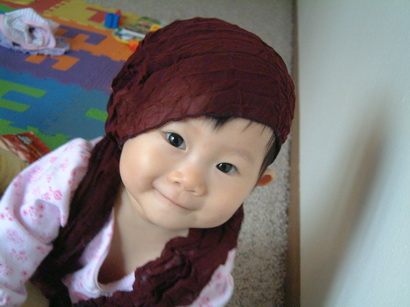
\includegraphics[bb=0 0 410 307,scale=.8]{dscf4684}
\caption{10个月大的Anna}
\label{fig:anna}
\end{figure}

上述代码中,\verb|[htbp]|~选项用来指定插图排版的理想位置,这几个字母分别代表~here、top、bottom、float page,也就是固定位置、页顶、页尾、单独的浮动页。我们可以使用这几个字母的任意组合,一般不推荐单独使用~\verb|[h]|,因为那个位置也许很不合适,\LaTeX~会很生气。

\verb|\centering|~用来使插图居中,\verb|\caption|~命令设置插图标题,\LaTeX~会自动给浮动环境的标题加上编号。注意~\verb|label|~应放在\verb|caption|~之后,否则引用时指向的是前一个插图。

\subsection{插入多幅图形}
\subsubsection{并排摆放,共享标题}
当我们需要两幅图片并排摆放,并共享标题时,可以在~\verb|figure|~环境中使用两个~\verb|\includegraphics|~命令。

\begin{fdemo}{
\centering
\includegraphics[scale=2]{examples/subfig_left.mps}
\includegraphics[scale=2]{examples/subfig_right.mps}
\captionof{figure}{反清复明}
}
\begin{figure}[htbp]
\centering
\includegraphics{left}
\includegraphics{right}
\caption{反清复明}
\end{figure}
\end{fdemo}

\subsubsection{并排摆放,各有标题}
如果想要两幅并排的图片各有自己的标题,可以在~\verb|figure|~环境中使用两个~\verb|minipage|~环境,每个环境里插入一个图。
\begin{code}
\begin{figure}[htbp]
\centering
\begin{minipage}[t]{0.3\textwidth}
    \centering
    \includegraphics{left}
    \caption{清明}
\end{minipage}
\end{code}
\begin{code}
\begin{minipage}[t]{0.3\textwidth}
    \centering
    \includegraphics{right}
    \caption{反复}
\end{minipage}
\end{figure}
\end{code}

\begin{figure}[htbp]
\centering
\begin{minipage}[t]{0.3\textwidth}
    \centering
    \includegraphics[scale=2]{examples/subfig_left.mps}
    \caption{清明}
\end{minipage}
\begin{minipage}[t]{0.3\textwidth}
    \centering
    \includegraphics[scale=2]{examples/subfig_right.mps}
    \caption{反复}
\end{minipage}
\end{figure}

\subsubsection{并排摆放,共享标题,各有子标题}
如果想要两幅并排的图片共享一个标题,并各有自己的子标题,可以使用~\verb|subfig|~宏包提供的~\verb|\subfloat|~命令。

\verb|subfloat|~命令缺少宽度参数。虽然我们可以用~\verb|\hspace|~命令调整子图的距离,子标题却只能和子图本身一样宽,就会出现折行。
\begin{code}
\usepackage{subfig}
\begin{figure}[htbp]
\centering
\subfloat[清明]{
    \label{fig:subfig_a}
    \includegraphics{left}
}
\hspace{80pt}
\subfloat[反复]{
    \label{fig:subfig_b}
    \includegraphics{right}
}
\caption{反清复明}
\end{figure}
\end{code}

每个子图可以有各自的引用,就象这个样子:\Fref{fig:subfig_a}、\Fref{fig:subfig_b}。
\begin{figure}[htbp]
\centering
\subfloat[清明]{
    \label{fig:subfig_a}
    \includegraphics[scale=2]{examples/subfig_left.mps}
}
\hspace{80pt}
\subfloat[反复]{
    \label{fig:subfig_b}
    \includegraphics[scale=2]{examples/subfig_right.mps}
}
\caption{反清复明}
\end{figure}

\subsubsection{改进的子图方法}
为了避免子标题折行,我们可以在~\verb|\subfloat|~里再嵌套个~\verb|minipage|,因为后者是有宽度的。
\begin{code}
\begin{figure}[htbp]
\centering
\subfloat[清明]{
\label{fig:improved_subfig_a}
\begin{minipage}[t]{0.3\textwidth}
    \centering
    \includegraphics{left}
\end{minipage}
}
\subfloat[反复]{
\label{fig:improved_subfig_b}
\begin{minipage}[t]{0.3\textwidth}
    \centering
    \includegraphics{right}
\end{minipage}
}
\caption{反清复明}
\end{figure}
\end{code}

\begin{figure}[htbp]
\centering
\subfloat[清明]{
\begin{minipage}[t]{0.3\textwidth}
    \centering
    \includegraphics[scale=2]{examples/subfig_left.mps}
\end{minipage}
}
\subfloat[反复]{
\begin{minipage}[t]{0.3\textwidth}
    \centering
    \includegraphics[scale=2]{examples/subfig_right.mps}
\end{minipage}
}
\caption{反清复明}
\end{figure}

\section{图形绘制工具比较}
与~\LaTeX~配套使用的绘图工具主要有三种:\MP、PSTricks~和~PGF,它们的特点如下。

\begin{itemize}
\item 工作方式。\MP~离线绘图,生成的~EPS~可以插入~\LaTeX~文档;PSTricks~和~PGF~都采用在线绘图的方式,也就是~\LaTeX~文档内直接使用绘图命令。
\item 兼容性。\MP~生成的~MPS~需要先转为~PDF~才能被~pdf\LaTeX~使用;PSTricks~生成的~EPS和~pdf\LaTeX~不兼容;PGF~提供针对各种~driver~的接口,兼容性最好。
\item 功能。PSTricks~有~PS~作后盾,功能最强;\MP~擅长处理数学内容;PGF~的流程图有独到之处。
\end{itemize}

限于篇幅,本文只对这三种工具进行简介。除了它们,用户也可以考虑一些面向~\LaTeX~的绘图前端,比如~Unix/Linux~下的~xfig~和~Windows~下的~TpX;或可以输出~EPS~的专用软件,比如~gnuplot~和~Matlab。

\section{\MP}
\label{sec:mp}

1989~年~John D. Hobby\footnote{Hobby 1985年从斯坦福获博士学位,导师就是Knuth,现供职于贝尔实验室。}开始设计一种绘图语言及其编译器,也就是~\MP。\MP~从~\MF~那里获得了大量灵感和源代码,学生从导师那里顺点东西自然是手到擒来。\MP~和~\MF~语法类似,\MP~的主要优点在于是它输出的是~EPS,而且支持彩色;\MF~输出的是点阵格式,不支持彩色。Knuth~声称自己画图时只用~\MP。

从~Hobby~主页上~\MP~的更新记录看,它的最后版本是~0.63,年份是~1994。目前~Taco Hoekwater\footnote{他也是LuaTeX开发者之一。}继续~\MP~的开发工作,最新版本是~1.005。

本文只对~\MP~作简单介绍,若想深入了解请参阅~Hobby~的《A User's Manual for MetaPost》\citep{Hobby_2007}。

\subsection{准备工作}
用户一般需要把~\MP~源文件(.mp)用一个命令行程序~\verb|mpost|~编译为一种特殊的~EPS,也称作~MPS,然后再把~MPS~插入~\LaTeX~源文件中使用。
\begin{figure}[htbp]
\centering
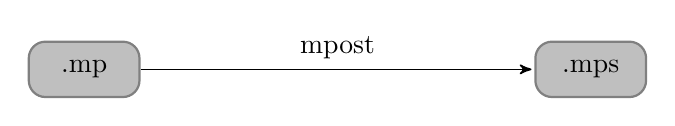
\begin{tikzpicture}
    \node[box] (mp) {.mp};
    \node[box, right=5 of mp] (mps) {.mps};
    \path (mp) edge [arrow] node[auto] {mpost} (mps);
\end{tikzpicture}
\caption{MetaPost~的编译}
\label{fig:mp}
\end{figure}

一个~\MP~源文件可以包含多个图形,一般形式如下。代码中每行语句以~\verb|;|~结尾,注释行以~\verb|%|~起始。每个图形的绘图命令包含在一对起始和结尾声明之间。文件结尾也要有一个结尾声明。
\begin{code}
beginfig(1); %图形起始
...          %绘图命令
endfig;      %图形结尾

beginfig(2);
...
endfig;
...
end;         %文件结尾
\end{code}

假如上面的源文件名字是~\verb|fig.mp|,我们可以执行以下编译命令。
\begin{code}
mpost fig(.mp)
\end{code}

编译后就会生成“fig.1、fig.2、$\cdots$”~等文件,每个文件的后缀就是相应的图形起始声明的编号。所以此编号在一个源文件中应保持唯一,否则后生成的文件就会覆盖前面的。

这样的文件名管理起来很麻烦,插入它们时也不能省略后缀,因为~\LaTeX~不能识别它们。用~\verb|\DeclareGraphicsExtensions|~来逐一声明后缀看起来很傻,自己改文件名更傻,\verb|\DeclareGraphicsRule|~也显得不够严谨。

然而~\MP~已经考虑到这个问题,为此提供了一个文件名模板命令。把下面的代码加到源文件头部,编译输出的文件名就会是“fig-01.mps、fig-02.mps、$\cdots$”。
\begin{code}
filenametemplate "%j-%2c.mps";   %加在源文件头部
\end{code}

我们也可以把这个命令加在每个图形的起始声明之前,指定个性化的输出文件名,这样可能更便于记忆。
\begin{code}
filenametemplate "flowchart.mps" %加在每个图形前面
\end{code}

MPS~可以用~GSview~查看,我们也可以用以下命令把它转为~PDF~再用~Adobe Reader~查看。

\begin{code}
epstopdf flowchart.mps
\end{code}

\subsection{基本图形对象}
为了节省空间,本节后面的示例会略去图形起始声明和结尾声明等不重要的细节。

\subsubsection{直线}

绘图命令~\verb|draw|~把几个点以直线段连接起来。\MP~中的缺省长度单位是~bp,用户也可以使用\Fref{tab:unit}~中的其它单位。我们还可以定义一个缩放系数,把坐标都转换成此系数的倍数,这样以后想缩放图形时只要改这个系数即可。

注意~\MP~中的变量赋值符号是~\verb|:=|,而~\verb|=|~用于方程式。变量在同一源文件中只须定义一次,其后的图形中都可以使用。

\begin{fdemo}{\includegraphics{examples/line.mps}}
draw (0,0)--(40,0)--(20,20)--(0,0);
u:=10pt; %缩放系数
draw (5u,0)--(9u,0)--(7u,2u)--cycle;
\end{fdemo}

几段直线或曲线可以构成一条路径(path),在路径末尾加个~\verb|cycle|~就能构成封闭路径(closed path)。上例中的两个三角形看起来都是封闭的,但是前面这个其实不是真正的封闭路径。

\subsection{点和线宽}
\verb|drawdot|~命令可以在指定坐标画一个点,为了使它醒目些我们可以换支粗一点的画笔。\MP~中的画笔缺省是直径~0.5pt~的圆形,拿它画出来的线宽就是~0.5pt。

\begin{fdemo}{\includegraphics{examples/dot.mps}}
draw (0,0)--(10u,4u);
pickup pencircle scaled 2pt;
drawdot (0,0);
drawdot (10u,4u);
\end{fdemo}

上面的~\verb|pickup|~是一种全局操作,也就是说它会影响到之后所有的绘图命令,我们也可以用~\verb|withpen|~为单个绘图命令设置画笔。

\begin{code}
draw (0,0)--(10u,4u) withpen pencircle scaled 2pt;
\end{code}

\subsubsection{曲线}
曲线和直线的命令相近,只是把连接两个点的~\verb|--|~换成了~\verb|..|。如果共用一些坐标,直线和曲线也可以混在一条语句里画。

\begin{fdemo}{\includegraphics{examples/curve.mps}}
draw (0,.5u)..(5u,3u)..(10u,1.5u)..
    (7u,0)..(5u,1.5u)..(7u,1.5u);
\end{fdemo}

\MP~的曲线用三次贝塞尔(Cubic B\'ezier)算法实现。用户可以在命令中增加~direction(方向)、Tension(张力)和~Curl(曲率)等控制,限于篇幅本文不赘述。

\subsubsection{预定义图形}
~\verb|fullcircle|~命令以原点为圆心画一个单位圆,类似的预定义图形还有~\verb|halfcircle、quartercircle、unitsquare|~等。注意单位正方形的参考点在左下而不在其中心。

通过不同的横向和纵向缩放系数,我们可以把圆形和正方形变成椭圆和长方形。

\begin{code}
draw fullcircle scaled 2u;
draw halfcircle scaled 2u shifted (3u,0);
draw quartercircle scaled 2u shifted (5u,0);
draw fullcircle xscaled 4u yscaled 2u shifted (9u,0);
draw unitsquare scaled 2u shifted (12u,-u);
draw unitsquare xscaled 4u yscaled 2u shifted (15u,-u);
\end{code}

\begin{out}
\includegraphics{examples/predefined.mps}
\end{out}

\subsection{图形控制}

\subsubsection{线型和箭头}
在绘制图形时,我们不仅可以变换线宽,也可以使用多种线型。
\begin{code}
draw (0,0)--(10u,0) dashed withdots;
draw (0,1u)--(10u,1u) dashed withdots scaled 2;
draw (0,2u)--(10u,2u) dashed evenly;
draw (0,3u)--(10u,3u) dashed evenly scaled 2;
\end{code}

\begin{out}
\includegraphics{examples/dashed.mps}
\end{out}

箭头和直线、曲线的语法相近,注意画反向箭头时需要把两个坐标用一对~\verb|()|~括起来。

\begin{fdemo}{\includegraphics{examples/arrow.mps}}
drawarrow (0,4u)--(9u,4u);
drawarrow reverse ((0,2u)--(9u,2u));
drawdblarrow (0,0)--(9u,0);
\end{fdemo}

\subsubsection{颜色和填充}
\MP~预定义的颜色有黑、白、红、绿、蓝,它们的~RGB~值分别为(0,0,0)、(1,1,1)、(1,0,0)、(0,1,0)、(0,0,1),缺省色就是黑色。

绘图命令一般都可以通过~\verb|withcolor|~参数来使用各种颜色。封闭路径可以用~\verb|fill|~命令填充。

\begin{fdemo}{\includegraphics{examples/color.mps}}
draw (0,4u)--(9u,4u) withcolor red;
draw (0,2u)--(9u,2u) withcolor green;
draw (0,0)--(9u,0) withcolor blue;
\end{fdemo}

\begin{code}
fill p scaled u;
fill p scaled u shifted (3u,0) withcolor red;
fill p scaled u shifted (6u,0) withcolor green;
fill p scaled u shifted (9u,0) withcolor blue;
\end{code}

\begin{out}
\includegraphics{examples/fill.mps}
\end{out}

另一个命令~\verb|filldraw|~可以看作是~\verb|fill+draw|,它除了填充外还会把路径用指定的画笔画一遍。然而不幸的是画边缘和填充内部只能用同一种颜色,所以它的用处不大。

除了为每个绘图命令单独指定颜色,我们也可以使用一个全局命令,使得其后的绘图命令都使用某种颜色。
\begin{code}
drawoption(withcolor blue);
\end{code}

下面的方法可以用来定义基本色以外的颜色,用基本色混色或直接用RGB值效果是一样的。

\begin{code}
color c[];
c1 := .9red + .6green + .3blue;
c2 := (.9,.6,.3);
\end{code}

\subsubsection{图形变换}
我们可以对路径进行缩放、平移、旋转等变换操作,横向和纵向缩放可以分开进行。由于旋转是围绕原点进行的,所以要注意平移和旋转的顺序。下例中定义了一个~\verb|path|~变量,以便后面重用。

\begin{code}
path p;
p := (0,0)--(2,0)--(1,1.732)--cycle;
draw p scaled u;
draw p xscaled 2u yscaled u shifted (3u,0);
draw p scaled u rotated 60 shifted (8u,0);
\end{code}

\begin{out}
\includegraphics{examples/transform.mps}
\end{out}

\subsubsection{标注}
\verb|\label|~命令可以在指定的点附近加文字标注。\MP~也可以用一对~\verb|btex|~和~\verb|etex|~来嵌入一些~\TeX~内容,比如数学标注。

\begin{code}
draw unitsquare xscaled 10u yscaled 4u;
label.top("top", (5u,4u));
label.bot("bottom", (5u,0));
label.lft("left", (0,2u));
label.rt("right", (10u,2u));
\end{code}
\begin{code}
label.ulft("upper left", (0,4u));
label.urt("upper right", (10u,4u));
label.llft("lower left", (0,0));
label.lrt("lower right", (10u,0));
label.rt(btex $E=mc^2$ etex, (3u,2u));
\end{code}

\begin{out}
\includegraphics{examples/label.mps}
\end{out}

因为用缺省方法编译生成的~MPS~不嵌入字体,当~\MP~包含文字时,GSview~就不能正常查看。这时我们可以给编译命令加个参数,生成的~MPS~就会包含字体信息。注意这种方法生成的~MPS~虽然~GSview~能查看,\verb|dvipdfmx|~却不能正常处理。

\begin{code}
mpost \prologues:=2; input fig.mp
\end{code}

\subsection{编程功能}

\subsubsection{数据类型和变量}
\MP~中有10~种基本数据类型:numeric、pair、path、pen、~color~、cmykcolor、transform、string、boolean、picture。我们已经接触过其中几种,比如缩放系数~u~就是一个~numeric,一个点的坐标是一个~pair,几个点用直线或曲线连起来是一个~path,pencircle~是一种~pen,black~是一种~color,scaled、rotated、shifted~都是~transform。

numeric~类型变量的精度是~1/65536,它的绝对值不能超过~4096,在计算过程中数值可以达到~32768。这样的规定也应归功于当年的电脑硬件,不过对于科技文档插图而言,4096~一般还是够用的。

除了缺省的~numeric,其它变量在使用之前都需要用数据类型来显式声明。相同类型的变量可以在一行语句中声明,但是带下标的变量不能放在同一行(这个规定很蹊跷)。
\begin{code}
numeric x,y,z;    %正确
numeric x1,x2,x3; %错误
numeric x[];      %正确
\end{code}

\subsubsection{数学运算}
\MP~中可以使用普通的运算符,比如~\verb|+ - * /|;也提供一些特殊的运算符,比如~\verb|a++b|~表示$\sqrt{a^2+b^2}$,\verb|a+-+b|~表示$\sqrt{a^2-b^2}$;另外\Fref{tab:math_function}~列出一些常用数学函数。

\begin{table}[htbp]
\caption{数学函数}
\label{tab:math_function}
\centering
\begin{tabular}{llll}
    \toprule
    abs     & 绝对值   & mexp & 指数 \\
    round   & 四舍五入 & mlog & 对数 \\
    ceiling & 向上圆整 & sind & 正弦 \\
    floor   & 向下圆整 & cosd & 余弦 \\
    mod     & 模余     & normaldeviate & 正态分布随机数 \\
    sqrt    & 开方     & uniformdeviate & 均匀分布随机数 \\
    \bottomrule
\end{tabular}
\end{table}

\subsubsection{循环}
当执行重复任务时,循环语句可以让程序变得简洁。注意下例中的循环语句是一条命令,之所以分成三行写是为了看起来清晰点。

\begin{fdemo}{\includegraphics{examples/loop.mps}}
draw (0,0) %注意这里没有分号
for x=1 upto 3: 
    ..(x*x,x)*u 
endfor;
\end{fdemo}

循环语句缺省步长是~1,我们也可以改用其它步长。\verb|upto|~其实就是~\verb|step 1 until|~的缩写方式。
\begin{code}
for x=1 step .5 until 3: 
\end{code}

\section{PSTricks}
\label{sec:pstricks}

PSTricks~是一个基于~PS~的宏包,有了它用户就可以直接在~\LaTeX~文档中插入绘图命令。PSTricks~早期的作者是~Timothy Van Zandt\footnote{法国Insead大学经济系教授。},初始开发年月不详,他于~1997~年退居二线,之后由~Denis Girou、Sebastian Rahtz\footnote{牛津大学计算机系网管。}、Herbert Voß~等维护。

本文只介绍~PSTricks~的基本功能,若想深入了解请参阅~Van Zandt~的《PSTricks User's Guide》\citep{Zandt_2007}。另外\Fref{tab:pst_add}~列出了一些可以和~PsTricks~配合使用的辅助宏包。

\begin{table}[htbp]
\caption{PSTricks~辅助宏包}
\label{tab:pst_add}
\centering
\begin{tabular}{llll}
    \toprule
    multido & 循环语句    & pst-eucl & 几何函数 \\    
    pst-plot & 函数绘图   & pst-math & 弧度三角函数 \\
    pst-plot3d & 三维绘图 & pstricks-add & 极坐标 \\  
    \bottomrule
\end{tabular}
\end{table}

\subsection{准备工作}
首先要引入~PSTricks~宏包。PSTricks~中缺省长度单位是~1cm,我们也可以设置自己的单位。
\psset{unit=10pt}
\begin{code}
\usepackage{pstricks}
\psset{unit=10pt}
\end{code}

绘图命令一般要放在~\verb|pspicture|~环境里,这样~\LaTeX~就会给图形预留一个矩形区域,注意这个矩形要能容纳所有图形对象。为了节省空间,在本节后面的示例代码中,~\verb|pspicture|~环境将被略去。

\begin{code}
\begin{pspicture}(0,0)(4,2)
...
\end{pspicture}
\end{code}

另外需要注意的是,嵌入~\LaTeX~的~PSTricks~生成的是~PS,\verb|dvips|~可以处理,\verb|dvipdfm|~和pdf\LaTeX~则不能。所以如果使用后两种~driver,需要先行生成~EPS。

第一种方法是把~PSTricks~代码放进一个空白的\LaTeX~页面,用它生成一个简单的~DVI。

\begin{code}
\documentclass{article}
\usepackage{pstricks}
\pagestyle{empty}   %页面样式为空

\begin{document}
\psset{unit=10pt}
\colorbox{white}{%
    \begin{pspicture}(0,0)(4,2)%
    \psdot(0,0)%
    \psdots(0,2)(2,2)(4,2)%
    \end{pspicture}%
}
\end{document}
\end{code}

然后用以下命令把~DVI~转为~EPS,\verb|-E|~参数即代表~EPS。上面代码中的~colorbox~使得生成的~EPS~有正确的范围框。

\begin{code}
dvips pst_dots(.dvi) -E -o dots.eps
\end{code}

第二种方法是用~\verb|pst-eps|~宏包,它能够在线处理~PSTricks~代码并生成~EPS,这样用户就可以在同一文件中使用该~EPS。

然而~\verb|dvipdfmx|~不能正确处理~\verb|pst-eps|~生成的~EPS。它和~\verb|\rput|、\verb|\uput|~命令,\verb|pst-plot|~宏包中的~\verb|\psaxes|~命令都不兼容。类似的~\verb|ps4pdf|~宏包和~\verb|tabularx|~宏包不兼容。

\begin{comment}
\usepackage{pst-eps}
\PSTtoEPS[bbllx=0,bblly=0,bburx=4,bbury=2,makeeps=all]
{dots.eps}{
    \psdot(0,0)
    \psdots(0,2)(2,2)(4,2)
}
\includegraphics{dots.eps}
\end{comment}

\subsection{基本图形对象}
\subsubsection{点}
我们可以用以下命令画一个或多个点。
\begin{comment}
\PSTtoEPS[bbllx=0,bblly=0,bburx=4,bbury=2,makeeps=all]
{examples/dot.eps}{
    \psdot(0,0)
    \psdots(0,2)(2,2)(4,2)
}
\end{comment}

\begin{fdemo}{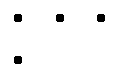
\includegraphics{examples/pst_dot.eps}}
\psdot(0,0)
\psdots(0,2)(2,2)(4,2)
\end{fdemo}

\subsubsection{直线、多边形、矩形}
\verb|\psline|~命令把多个点用直线段连接起来,线段之间的连接缺省为尖角,也可以设置圆角。
\begin{comment}
\PSTtoEPS[bbllx=0,bblly=0,bburx=9,bbury=2,makeeps=all]
{examples/line.eps}{
    \psline(0,0)(2,2)(4,0)
    \psline[linearc=.3](5,0)(7,2)(9,0)
}
\end{comment}

\begin{fdemo}{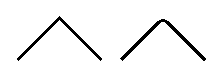
\includegraphics{examples/pst_line.eps}}
\psline(0,0)(2,2)(4,0)
\psline[linearc=.3](5,0)(7,2)(9,0)
\end{fdemo}

\verb|\pspolygon|~命令和~\verb|\psline|~类似,但是它会形成封闭路径。
\begin{comment}
\PSTtoEPS[bbllx=0,bblly=0,bburx=9,bbury=2,makeeps=all]
{examples/polygon.eps}{
    \pspolygon(0,0)(2,2)(4,0)
    \pspolygon[linearc=.3](5,0)(7,2)(9,0)
}
\end{comment}

\begin{fdemo}{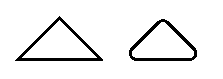
\includegraphics{examples/pst_polygon.eps}}
\pspolygon(0,0)(2,2)(4,0)
\pspolygon[linearc=.3](5,0)(7,2)(9,0)
\end{fdemo}

矩形用~\verb|\psframe|~命令,其参数就是矩形左下角和右上角的坐标。矩形也可以设置圆角。
\begin{comment}
\PSTtoEPS[bbllx=0,bblly=0,bburx=9,bbury=2,makeeps=all]
{examples/frame.eps}{
    \psframe(0,0)(4,2)
    \psframe[framearc=.3](5,0)(9,2)
}
\end{comment}

\begin{fdemo}{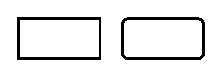
\includegraphics{examples/pst_frame.eps}}
\psframe(0,0)(4,2)
\psframe[framearc=.3](5,0)(9,2)
\end{fdemo}

\subsubsection{圆、椭圆、圆弧、扇形}
圆形用~\verb|\pscircle|~命令,参数是圆心和半径。椭圆用~\verb|\psellipse|~命令,参数是中心、长径、短径。注意这两个命令的半径参数用不同的括号,可能是作者的笔误。
\begin{comment}
\PSTtoEPS[bbllx=0,bblly=0,bburx=7,bbury=2,makeeps=all]
{examples/circle.eps}{
    \pscircle(1,1){1}
    \psellipse(5,1)(2,1)
}
\end{comment}

\begin{fdemo}{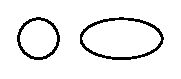
\includegraphics{examples/pst_circle.eps}}
\pscircle(1,1){1}
\psellipse(5,1)(2,1)
\end{fdemo}

圆弧用~\verb|\psarc|~命令,其参数是圆心、半径、起止角度,逆时针作图。~\verb|\psarcn|~类似,只是顺时针作图。扇形用~\verb|\pswedge|~命令。
\begin{comment}
\PSTtoEPS[bbllx=0,bblly=0,bburx=11,bbury=2,makeeps=all]
{examples/arc.eps}{
    \psarc(1,0){2}{0}{120}
    \psarcn(5,0){2}{120}{0}
    \pswedge(9,0){2}{0}{120}
}
\end{comment}

\begin{fdemo}{\includegraphics{examples/pst_arc.eps}}
\psarc(1,0){2}{0}{120}
\psarcn(5,0){2}{120}{0}
\pswedge(9,0){2}{0}{120}
\end{fdemo}

\subsubsection{曲线}
\verb|\pscurve|~命令把一系列点用平滑曲线连接起来;它的变形版本~\verb|\psecurve|~命令不显示曲线的两个端点;另一变形命令~\verb|\psccurve|~则把曲线封闭起来。

参数~\verb|showpoints=true|~用来显示曲线的构成点,此参数也可用于其它绘图命令。
\begin{comment}
\PSTtoEPS[bbllx=0,bblly=0,bburx=15,bbury=2,makeeps=all]
{examples/curve.eps}{
    \pscurve[showpoints=true](0,1)(1,2)(3,0)(4,2)(1,0)
    \psecurve[showpoints=true](5,1)(6,2)(8,0)(9,2)(5,0)
    \psccurve[showpoints=true](11,1)(12,2)(14,0)(15,2)(12,0)
}
\end{comment}

\begin{code}
\pscurve[showpoints=true](0,1)(1,2)(3,0)(4,2)(1,0)
\psecurve[showpoints=true](5,1)(6,2)(8,0)(9,2)(5,0)
\psccurve[showpoints=true](11,1)(12,2)(14,0)(15,2)(12,0)
\end{code}
\begin{out}
\includegraphics{examples/pst_curve.eps}
\end{out}

\verb|\psbezier|~命令输出一条贝塞尔曲线,其参数就是曲线的控制点。
\begin{comment}
\PSTtoEPS[bbllx=0,bblly=0,bburx=6,bbury=2,makeeps=all]
{examples/bezier.eps}{
    \psbezier[showpoints=true]
        (0,0)(2,2)(4,0)(6,2)
}
\end{comment}

\begin{fdemo}{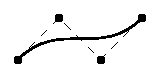
\includegraphics{examples/pst_bezier.eps}}
\psbezier[showpoints=true]
    (0,0)(2,2)(4,0)(6,2)
\end{fdemo}

抛物线用~\verb|\psparabola|~命令,它有两个参数,第一个是抛物线通过的一点,第二个是抛物线的顶点。
\begin{comment}
\PSTtoEPS[bbllx=0,bblly=0,bburx=2,bbury=2,makeeps=all]
{examples/parabola.eps}{
    \psparabola[showpoints=true]
        (2,2)(1,0)
}
\end{comment}

\begin{fdemo}{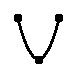
\includegraphics{examples/pst_parabola.eps}}
\psparabola[showpoints=true]
    (2,2)(1,0)
\end{fdemo}

\subsubsection{网格和坐标}
科技制图通常会用到坐标网格。\verb|\psgrid|~命令输出一个矩形网格,它有三个参数点。网格坐标标注在通过第一个点的两条直线上,第二和第三个点是矩形的两个对角顶点。当第一个参数省略时,坐标标注在通过第一个顶点的两条矩形边上。
\begin{comment}
\psset{unit=10pt}
\PSTtoEPS[bbllx=-1,bblly=-1,bburx=8.4,bbury=2.4,makeeps=all]
{examples/grid.eps}{
    \psgrid(0,0)(-1,-1)(3,2)
    \psgrid(5,0)(8,2)
}
\end{comment}

\begin{code}
\psgrid(0,0)(-1,-1)(3,2)
\psgrid(5,0)(8,2)
\end{code}
\begin{out}
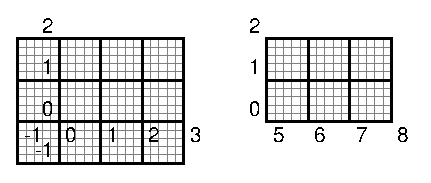
\includegraphics{examples/pst_grid.eps}
\end{out}

\verb|pst-plot|~宏包提供的~\verb|\psaxes|~命令输出坐标轴。它的参数和~\verb|\psgrid|~的类似,刻度和标注都可以灵活地设置,也可以把坐标轴改成一个矩形框的形式。
\begin{code}
\psset{unit=10pt}
\psaxes{<->}(0,0)(-1,-1)(3,2)
\psaxes[tickstyle=top,labels=none]{->}(5,0)(8,2)
\psaxes[axesstyle=frame,tickstyle=top]{->}(10,0)(13,2)
\end{code}
\begin{out}
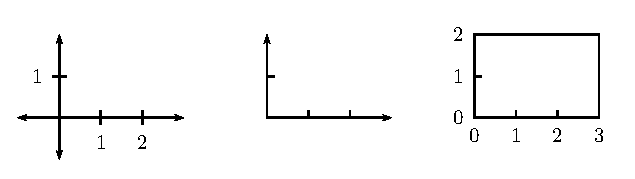
\includegraphics{examples/pst_axis.eps}
\end{out}

\subsection{图形控制}
\subsubsection{线型和箭头}
PSTricks~中的缺省线宽是~0.8pt,缺省线型是实线。以下参数可以控制单个绘图命令的线宽和线型。
\begin{comment}
\psset{unit=10pt}
\PSTtoEPS[bbllx=0,bblly=0,bburx=9,bbury=4,makeeps=all]
{examples/linestyle.eps}{
    \psline[linewidth=1.5pt](0,4)(9,4)
    \psline[linestyle=dotted](0,2)(9,2)
    \psline[linestyle=dashed](0,0)(9,0)
}
\end{comment}

\begin{fdemo}{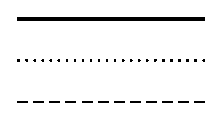
\includegraphics{examples/pst_linestyle.eps}}
\psline[linewidth=1.5pt](0,4)(9,4)
\psline[linestyle=dotted](0,2)(9,2)
\psline[linestyle=dashed](0,0)(9,0)
\end{fdemo}

我们也可以用命令~\verb|\psset|~命令来设置全局参数。
\begin{code}
\psset{linewidth=1pt,linestyle=dashed}
\end{code}

以下参数可以控制绘图命令的箭头。
\begin{comment}
\PSTtoEPS[bbllx=0,bblly=0,bburx=9,bbury=4,makeeps=all]
{examples/arrow.eps}{
    \psline{->}(0,4)(9,4)
    \psline{<-}(0,2)(9,2)
    \psline{<->}(0,0)(9,0)
}
\end{comment}

\begin{fdemo}{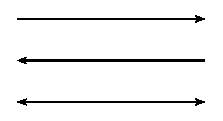
\includegraphics{examples/pst_arrow.eps}}
\psline{->}(0,4)(9,4)
\psline{<-}(0,2)(9,2)
\psline{<->}(0,0)(9,0)
\end{fdemo}

\subsubsection{颜色和填充}
PSTricks~预定义的颜色有~black、darkgray、gray、lightgray、white~等灰度颜色,也有~red、green、blue、cyan、magenta、yellow~等彩色。我们也可以自定义灰度颜色和彩色。

\begin{code}
\newgray{mygray}{.3}
\newrgbcolor{mycolor}{.3 .4 .5}
\end{code}

以下参数可以控制单个绘图命令的颜色,我们也可以用~\verb|\psset|~命令设置全局参数。
\begin{comment}
\PSTtoEPS[bbllx=0,bblly=0,bburx=9,bbury=4,makeeps=all]
{examples/color.eps}{
    \psline[linecolor=red](0,4)(9,4)
    \psline[linecolor=green](0,2)(9,2)
    \psline[linecolor=blue](0,0)(9,0)
}
\end{comment}

\begin{fdemo}{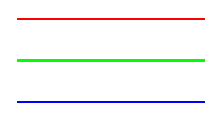
\includegraphics{examples/pst_color.eps}}
\psline[linecolor=red](0,4)(9,4)
\psline[linecolor=green](0,2)(9,2)
\psline[linecolor=blue](0,0)(9,0)
\end{fdemo}

以下参数可以控制单个绘图命令的填充模式和填充颜色,注意只有封闭路径才可以填充。
\begin{comment}
\PSTtoEPS[bbllx=0,bblly=0,bburx=11,bbury=2,makeeps=all]
{examples/fill.eps}{
    \pscircle[fillstyle=solid,fillcolor=red](1,1){1}
    \pscircle[fillstyle=vlines](4,1){1}
    \pscircle[fillstyle=hlines](7,1){1}
    \pscircle[fillstyle=crosshatch](10,1){1}
}
\end{comment}

\begin{code}
\pscircle[fillstyle=solid,fillcolor=red](1,1){1}
\pscircle[fillstyle=vlines](4,1){1}
\pscircle[fillstyle=hlines](7,1){1}
\pscircle[fillstyle=crosshatch](10,1){1}
\end{code}
\begin{out}
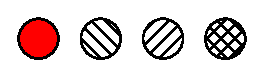
\includegraphics{examples/pst_fill.eps}
\end{out}

\subsection{对象布局}
\subsubsection{平移}
参数~\verb|origin|~可以让一个图形对象平移到指定的坐标点,我们也可以用~\verb|\psset|~命令设置全局平移参数。
\begin{comment}
\PSTtoEPS[bbllx=0,bblly=0,bburx=7,bbury=2,makeeps=all]
{examples/origin.eps}{
    \psframe(0,0)(3,2)
    \psframe[origin={4,0}](0,0)(3,2)
}
\end{comment}

\begin{fdemo}{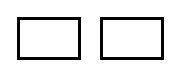
\includegraphics{examples/pst_origin.eps}}
\psframe(0,0)(3,2)
\psframe[origin={4,0}](0,0)(3,2)
\end{fdemo}

\subsubsection{旋转}
\verb|\rput|~命令可以对一个图形对象同时进行旋转和平移操作。它有两个参数,第一个是旋转角度,第二个是平移到的坐标点。
\begin{fdemo}{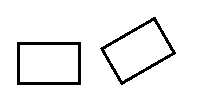
\includegraphics{examples/pst_rput.eps}}
\psframe(0,0)(3,2)
\rput{30}(5,0){\psframe(0,0)(3,2)}
\end{fdemo}

\subsubsection{文字标注}
\verb|\rput|~命令还可以在指定的坐标点标注文字,这时它的第一个参数是坐标点相对于标注的位置。其取值可以是纵向的~t、b(上下),或横向的~l、r(左右),也可以是纵向和横向位置的组合。
\begin{fdemo}{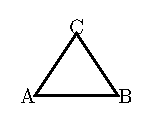
\includegraphics{examples/pst_label.eps}}
\pspolygon(0,0)(4,0)(2,3)
\rput[r](0,0){A}
\rput[l](4,0){B}
\rput[b](2,3){C}
\end{fdemo}

\verb|\rput|~生成的标注就在坐标点上,有时会感觉离图形太近。另一个命令~\verb|\uput|~则生成缺省距离指定坐标点~5pt的标注,它的第一个参数是标注相对于坐标点的角度。
\begin{fdemo}{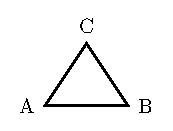
\includegraphics{examples/pst_uput.eps}}
\pspolygon(0,0)(4,0)(2,3)
\uput[l](0,0){A}
\uput[r](4,0){B}
\uput[u](2,3){C}
\end{fdemo}

\verb|\uput|~的角度参数可以是任意角度,也可以是字母,参见。注意~\verb|\uput|~的角度参数和~\verb|\rput|~命令的参考点位置参数的定义几乎正好相反,这也许反映了作者洒脱的风格。

\begin{table}[htbp]
\caption{uput~命令的角度参数}
\label{tab:uput}
\centering
\begin{tabular}{lrlr}
    \toprule
    r &   0$^\circ$ & ur &  45$^\circ$ \\
    u &  90$^\circ$ & ul & 135$^\circ$ \\
    l & 180$^\circ$ & dl & 225$^\circ$ \\
    d & 270$^\circ$ & dr & 315$^\circ$ \\
    \bottomrule
\end{tabular}
\end{table}

\section{PGF}
\label{sec:pgf}
PGF~和~Beamer~的作者都是~Till Tantau\footnote{德国Lübeck大学计算机研究所教授。}。Tantau~当初开发~Beamer~是为了应付~2003~年他的博士学位论文答辩,之后它在~CTAN~上流行开来。2005~年~PGF~从~Beamer~项目中分离出来,成为一个独立的宏包。

本文只对~PGF~作简单介绍,若想深入了解请参阅~Tantau~的《TikZ and PGF Manual》\citep{Tantau_2008}。

\subsection{准备工作}
一般人们并不直接使用~PGF~命令,而是通过它前端~TikZ~来调用~PGF。在引用~\verb|tikz|~宏包之前,用户需要设置~PGF~系统~driver。
\begin{code}
\def\pgfsysdriver{pgfsys-dvipdfmx.def}
\usepackage{tikz}
\end{code}

PGF~的缺省长度单位是~1cm,我们也可以改用其它单位。注意这样预定义的长度单位有时会失效,这可能是~PGF~的~bug。
\begin{code}
\pgfsetxvec{\pgfpoint{10pt}{0}}
\pgfsetyvec{\pgfpoint{0}{10pt}}
\end{code}

TikZ~提供一个~\verb|tikz|~命令和一个~\verb|tikzpicture|~环境,具体绘图指令可以放在~\verb|tikz|~后面,也可以放在~\verb|tikzpicture|~中间。两种方法效果相同,用户可以任意选择。为了节省空间,本节的示例将省略部分环境代码。
\begin{code}
\tikz ...   %绘图命令
\begin{tikzpicture}
...         %绘图命令
\end{tikzpicture}
\end{code}

\subsection{基本图形对象}
\subsubsection{直线、多边形、矩形}
TikZ~中直线的语法和~\MP~类似,加~\verb|cycle|~参数才能构成真正的封闭路径。
\begin{fdemo}{
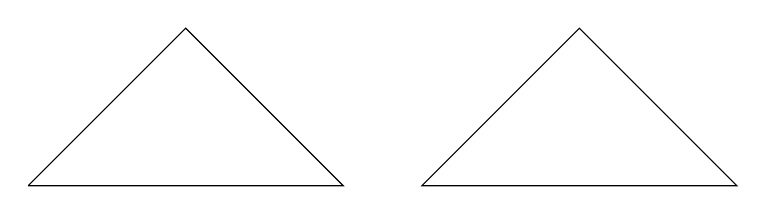
\begin{tikzpicture}
\draw (0,0)--(4,0)--(2,2)--(0,0);
\draw (5,0)--(9,0)--(7,2)--cycle;
\end{tikzpicture}
}
\draw (0,0)--(4,0)--(2,3)--(0,0);
\draw (5,0)--(9,0)--(7,3)--cycle;
\end{fdemo}

矩形命令如下,它的两个参数是矩形的两个对角顶点。
\begin{fdemo}{
\begin{tikzpicture}
\draw (0,0) rectangle (4,2);
\end{tikzpicture}
}
\draw (0,0) rectangle (4,2);
\end{fdemo}

\subsubsection{圆、椭圆、弧}
圆和椭圆命令如下,圆的参数是圆心和半径,椭圆的参数是中心、长径、短径。
\begin{fdemo}{
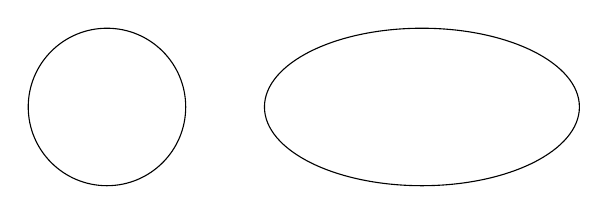
\begin{tikzpicture}
\draw (1,1) circle (1);
\draw (5,1) ellipse (2 and 1);
\end{tikzpicture}
}
\draw (1,1) circle (1);
\draw (5,1) ellipse (2 and 1);
\end{fdemo}

圆弧和椭圆弧命令如下,圆弧的参数是起始点,起始角度、终止角度、半径;椭圆弧则把半径换成了长径和短径。
\begin{fdemo}{
\begin{tikzpicture}
\draw (2,1) arc (0:270:1);
\draw (7,1) arc (0:270:2 and 1);
\end{tikzpicture}
}
\draw (2,1) arc (0:270:1);
\draw (7,1) arc (0:270:2 and 1);
\end{fdemo}

\subsubsection{曲线和抛物线}
曲线命令如下,中间的参数是控制点。
\begin{fdemo}{
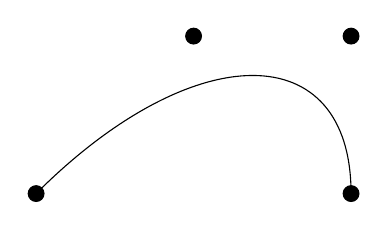
\begin{tikzpicture}
\draw (0,0) .. controls (2,2) 
    and (4,2) .. (4,0);
\filldraw (0,0) circle (.1)
    (2,2) circle (.1)
    (4,2) circle (.1)
    (4,0) circle (.1);
\end{tikzpicture}
}
\draw (0,0) .. controls (2,2) 
    and (4,2) .. (4,0);
\end{fdemo}

抛物线命令如下,除了起止点还可以指定顶点。
\begin{fdemo}{
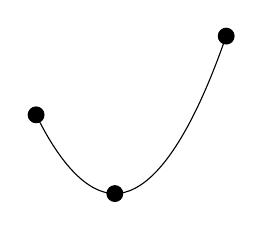
\begin{tikzpicture}
\draw (-1,1) parabola bend (0,0) (1.414,2);
\filldraw (-1,1) circle (.1)
    (0,0) circle (.1)
    (1.414,2) circle (.1);
\end{tikzpicture}
}
\draw (-1,1) parabola 
    bend (0,0) (1.414,2);
\end{fdemo}

\subsection{图形控制}
\subsubsection{线型和箭头}
绘图命令可以设置线型和箭头参数。
\begin{fdemo}{
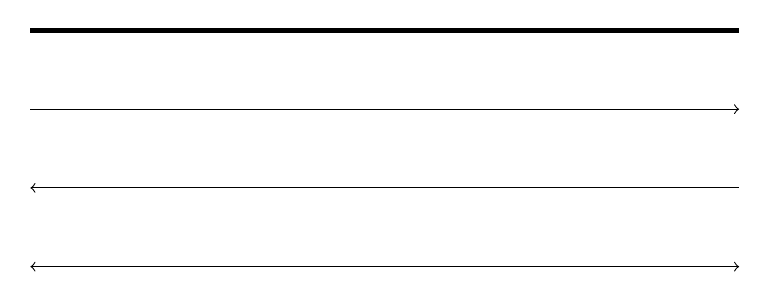
\begin{tikzpicture}
\draw[line width=2pt] (0,3)--(9,3);
\draw[->] (0,2)--(9,2);
\draw[<-] (0,1)--(9,1);
\draw[<->] (0,0)--(9,0);
\end{tikzpicture}
}
\draw[line width=2pt] (0,0)--(9,0);
\draw[->] (0,1)--(9,1);
\draw[<-] (0,2)--(9,2);
\draw[<->] (0,3)--(9,3);
\end{fdemo}

\subsubsection{颜色、填充、阴影}
颜色参数的用法如下。PGF~可以使用~\verb|xcolor|~宏包\citep{Kern_2007}中定义的所有颜色。
\begin{fdemo}{
\begin{tikzpicture}
\draw[red] (0,4)--(9,4);
\draw[green] (0,2)--(9,2);
\draw[blue] (0,0)--(9,0);
\end{tikzpicture}
}
\draw[red] (0,4)--(9,4);
\draw[green] (0,2)--(9,2);
\draw[blue] (0,0)--(9,0);
\end{fdemo}

封闭路径可以用颜色填充,\verb|\filldraw|~命令可以分别指定边框色和填充色。
\begin{fdemo}{
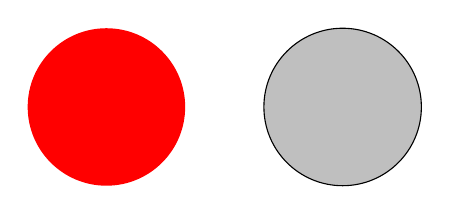
\begin{tikzpicture}
\fill[red] (1,1) circle (1);
\filldraw[fill=lightgray,draw=black] 
    (4,1) circle (1);
\end{tikzpicture}
}
\fill[red] (1,1) circle (1);
\filldraw[fill=lightgray,draw=black] 
    (4,1) circle (1);
\end{fdemo}

\verb|\shade|~命令可以产生渐变和光影效果,缺省是从上到下,灰色渐变为白色。我们也可以使用其它方向和颜色的渐变。
\begin{code}
\shade (0,0) rectangle (2,2);
\shade[left color=red,right color=orange] (3,0) rectangle (5,2);
\shade[inner color=red,outer color=orange] (6,0) rectangle (8,2);
\shade[ball color=blue] (10,1) circle (1);
\end{code}

\begin{out}
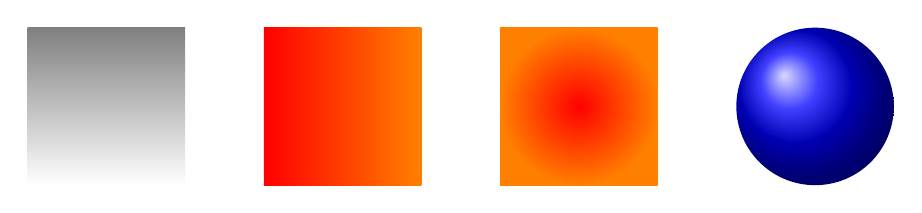
\begin{tikzpicture}
\shade (0,0) rectangle (2,2);
\shade[left color=red,right color=orange] (3,0) rectangle (5,2);
\shade[inner color=red,outer color=orange] (6,0) rectangle (8,2);
\shade[ball color=blue] (10,1) circle (1);
\end{tikzpicture}
\end{out}

\subsubsection{图形变换}
对图形对象可以进行平移和旋转操作,注意如果两种操作同时进行,它们是有顺序的。注意预定义的长度单位在这里对平移参数失效。
\begin{code}
\draw (0,0) rectangle (2,2);
\draw[xshift=30pt] (0,0) rectangle (2,2);
\draw[xshift=75pt,rotate=45] (0,0) rectangle (2,2);
\end{code}

\begin{out}
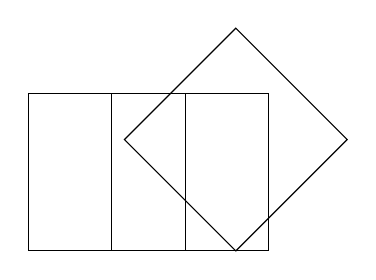
\begin{tikzpicture}
\draw (0,0) rectangle (2,2);
\draw[xshift=30pt] (0,0) rectangle (2,2);
\draw[xshift=75pt,rotate=45] (0,0) rectangle (2,2);
\end{tikzpicture}
\end{out}

\subsection{样式}
PGF~比~\MP~和~PSTricks~多了一个有趣的概念:样式(style),它的思路和~HTML~的~CSS~相近。我们可以先定义两种样式,
\tikzset{
    myline/.style={line width=2pt},
    myblueline/.style={myline,blue}
}
\begin{code}
\tikzset{
    myline/.style={line width=2pt},
    myblueline/.style={myline,blue}
}
\end{code}

然后就可以在绘图命令中这样使用样式。
\begin{fdemo}{
\begin{tikzpicture}
\draw[myline] (0,2)--(9,2);
\draw[myblueline] (0,0)--(9,0);
\end{tikzpicture}
}
\draw[myline] (0,2)--(9,2);
\draw[myblueline] (0,0)--(9,0);
\end{fdemo}

除了用~\verb|\tikzset|~命令定义样式,我们也可以在~\verb|tikzpicture|~环境头部声明样式。前者是全局性的,后者则是局部性的。
\begin{code}
\begin{tikzpicture}[
    thickline/.style=2pt,
    bluethickline/.style={thickline,color=blue}
]
...
\end{tikzpicture}
\end{code}

注意在样式中预定义长度单位有时会失效,所以最好使用绝对单位。

\subsection{流程图}
\subsubsection{节点}
PGF~中的节点(node)可以是简单的标签,也可以有各种形状的边框,还可以有各种复杂的属性。比如下例中的节点样式:\verb|box|,它的边框是矩形,有圆角;它有最小宽度、高度、文字和边框的距离,边框和填充颜色等属性。

\begin{code}
\tikzset{
    box/.style={rectangle, rounded corners=6pt, 
        minimum width=50pt, minimum height=20pt, inner sep=6pt, 
        draw=gray,thick, fill=lightgray}
}
\end{code}

除了上述类别属性,节点还可以有名字、位置等属性。在下例中,我们先画了三个有名字的文本框;然后用箭头把文本框连接起来,注意连接时要引用文本框的名字;接着在箭头上加了标签。
\begin{code}
\node[box] (tex) at(0,0) {.tex};  %文本框
\node[box] (dvi) at(10,0) {.dvi}; %文本框
\node[box] (pdf) at(20,0) {.pdf}; %文本框
\draw[->] (tex)--(dvi);           %箭头
\draw[->] (dvi)--(pdf);           %箭头
\node at (5,1) {latex};           %标签
\node at (15,1) {dvipdfmx};       %标签
\end{code}

\begin{out}
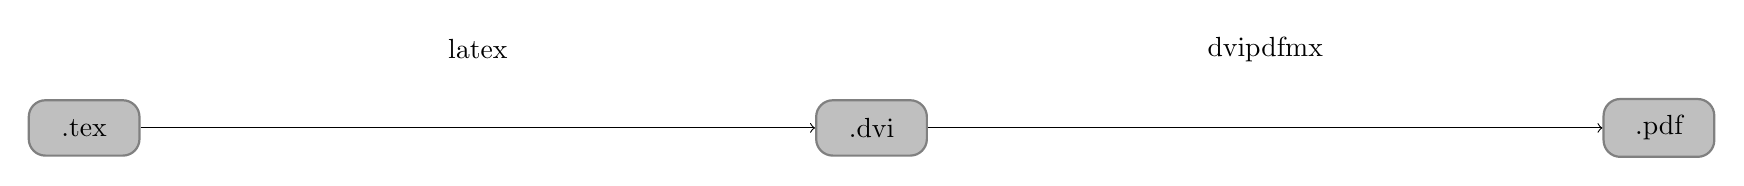
\begin{tikzpicture}
\node[box] (tex) at(0,0) {.tex};
\node[box] (dvi) at(10,0) {.dvi};
\node[box] (pdf) at(20,0) {.pdf};
\draw[->] (tex)--(dvi);
\draw[->] (dvi)--(pdf);
\node at (5,1) {latex};
\node at (15,1) {dvipdfmx};
\end{tikzpicture}
\end{out}

在上例中的节点都使用了绝对位置,PGF~中还可以使用更灵活一点的相对位置。比如在下例中,dvi~节点在~tex~节点右边~50pt~处(我们前面定义的基本长度单位是~10pt),而~pdf~节点又在~dvi~节点右边~50pt~处。

箭头可以换为专门用来连接节点的~\verb|edge|~;标签也改成相对位置,箭头上方~5pt~处。
\begin{code}
\node[box] (tex) {.tex};
\node[box,right=5 of tex] (dvi) {.dvi};
\node[box,right=6 of dvi] (pdf) {.pdf};
\path (tex) edge[->]  node[above=.5] {latex} (dvi)
    (dvi) edge[->] node[above=.5] {dvipdfmx} (pdf);
\end{code}

\begin{out}
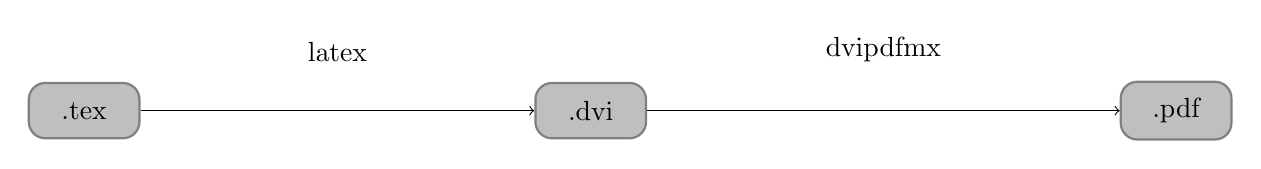
\begin{tikzpicture}
\node[box] (tex) {.tex};
\node[box,right=5 of tex] (dvi) {.dvi};
\node[box,right=6 of dvi] (pdf) {.pdf};
\path (tex) edge[->]  node[above=.5] {latex} (dvi)
    (dvi) edge[->] node[above=.5] {dvipdfmx} (pdf);
\end{tikzpicture}
\end{out}

\subsubsection{树}
下面是一棵简单的树。我们可以用一个参数控制相邻节点的距离,预定义长度单位对此参数也会失效。
\begin{code}
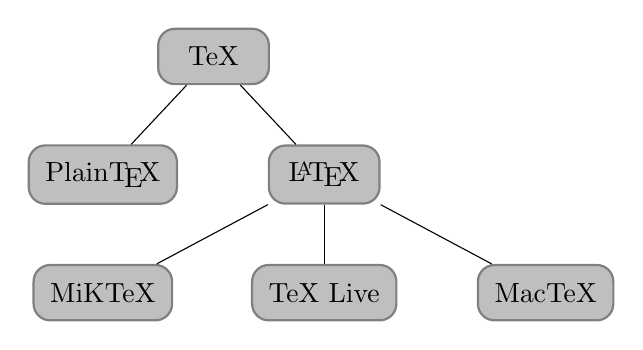
\begin{tikzpicture}[sibling distance=80pt]
\node[box] {TeX}
    child {node[box] {Plain\TeX}}
    child {node[box] {\LaTeX}
        child {node[box] {MiKTeX}}
        child {node[box] {TeX Live}}
        child {node[box] {MacTeX}}
    };
\end{tikzpicture}
\end{code}

\begin{out}
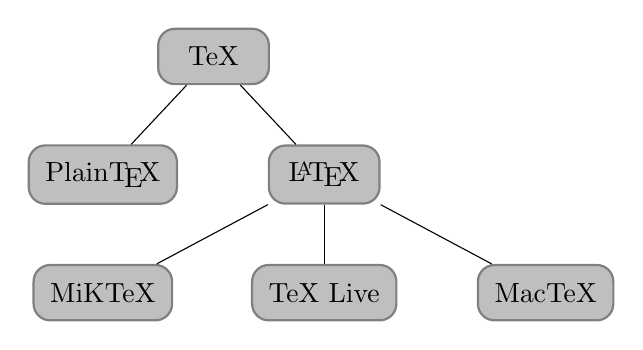
\begin{tikzpicture}[sibling distance=80pt]
\node[box] {TeX}
    child {node[box] {Plain\TeX}}
    child {node[box] {\LaTeX}
        child {node[box] {MiKTeX}}
        child {node[box] {TeX Live}}
        child {node[box] {MacTeX}}
    };
\end{tikzpicture}
\end{out}

\bibliographystyle{unsrtnat}
\bibliography{reading}
\newpage

\chapter{表格}
\label{sec:tables}

\section{简单表格}
\verb|tabular|~环境提供了最简单的表格功能。它用~\verb|\hline|~命令代表横线,\verb+|+~代表竖线,用~\verb|&|~来分栏。每个栏位的对齐方式可以用~l、c、r(左中右)来控制。
\begin{code}
\begin{tabular}{|l|c|r|}
    \hline 
    操作系统 & 发行版 & 编辑器 \\
    \hline 
    Windows & MikTeX & TeXnicCenter \\
    \hline 
    Unix/Linux & TeX Live & Emacs \\
    \hline 
    Mac OS & MacTeX & TeXShop \\
    \hline 
\end{tabular}
\end{code}

\begin{tabular}{|l|c|r|}
    \hline 
    操作系统 & 发行版 & 编辑器 \\
    \hline 
    Windows & MikTeX & TeXnicCenter \\
    \hline 
    Unix/Linux & TeX Live & Emacs \\
    \hline 
    Mac OS & MacTeX & TeXShop \\
    \hline 
\end{tabular}
\ \\

和针对插图的~\verb|figure|~环境类似,\LaTeX~还有另一个针对表格的浮动环境~\verb|table|。我们可以用它给上面的示例穿件马甲,顺便把表格简化为科技文献中常用的三线表。

\begin{code}
\begin{table}[htbp]
\caption{浮动环境中的三线表}
\label{tab:threesome}
\centering
\begin{tabular}{lll}
    \hline 
    操作系统 & 发行版 & 编辑器 \\
    \hline 
    Windows & MikTeX & TeXnicCenter \\
    Unix/Linux & TeX Live & Emacs \\
    Mac OS & MacTeX & TeXShop \\
    \hline 
\end{tabular}
\end{table}
\end{code}

\begin{table}[htbp]
\caption{浮动环境中的三线表}
\label{tab:threesome}
\centering
\begin{tabular}{lll}
    \hline 
    操作系统 & 发行版 & 编辑器 \\
    \hline 
    Windows & MikTeX & TeXnicCenter \\
    Unix/Linux & TeX Live & Emacs \\
    Mac OS & MacTeX & TeXShop \\
    \hline 
\end{tabular}
\end{table}

完美主义者可能觉得上面示例中的三条线一样粗不够美观,这时可以使用~\verb|booktabs|~宏包\citep{Fear_2005}的几个命令。

\begin{code}
\begin{table}[htbp]
\caption{浮动环境中的三线表}
\centering
\begin{tabular}{lll}
    \toprule
    操作系统 & 发行版 & 编辑器 \\
    \midrule
    Windows & MikTeX & TeXnicCenter \\
    Unix/Linux & TeX Live & Emacs \\
\end{code}

\begin{code}
    Mac OS & MacTeX & TeXShop \\
    \bottomrule
\end{tabular}
\end{table}
\end{code}

\begin{table}[htbp]
\caption{\texttt{booktabs}~宏包的效果}
\centering
\begin{tabular}{lll}
    \toprule
    操作系统 & 发行版 & 编辑器 \\
    \midrule
    Windows & MikTeX & TeXnicCenter \\
    Unix/Linux & TeX Live & Emacs \\
    Mac OS & MacTeX & TeXShop \\
    \bottomrule
\end{tabular}
\end{table}

\section{表格宽度}
有时我们需要控制某栏位宽度,可以将其对齐方式参数从~\verb|l、c、r|~改为~\verb|p{宽度}|~。
\begin{code}
\begin{table}[htbp]
\caption{控制栏位宽度}
\centering
\begin{tabular}{p{100pt}p{100pt}p{100pt}}
    \toprule
    操作系统 & 发行版 & 编辑器 \\
    \midrule
    Windows & MikTeX & TeXnicCenter \\
    Unix/Linux & TeX Live & Emacs \\
    Mac OS & MacTeX & TeXShop \\
    \bottomrule
\end{tabular}
\end{table}
\end{code}

\begin{table}[htbp]
\caption{控制栏位宽度}
\centering
\begin{tabular}{p{100pt}p{100pt}p{100pt}}
    \toprule
    操作系统 & 发行版 & 编辑器 \\
    \midrule
    Windows & MikTeX & TeXnicCenter \\
    Unix/Linux & TeX Live & Emacs \\
    Mac OS & MacTeX & TeXShop \\
    \bottomrule
\end{tabular}
\end{table}

若想控制整个表格的宽度可以使用~\verb|tabularx|~宏包,\verb|X|~参数表示某栏可以折行。

\begin{code}
\begin{table}[htbp]
\caption{控制表格宽度}
\centering
\begin{tabularx}{350pt}{lXlX}
    \toprule
    李白 & 平林漠漠烟如织,寒山一带伤心碧。暝色入高楼,有人楼上愁。玉梯空伫立,宿鸟归飞急。何处是归程,长亭更短亭。& 
    泰戈尔 & 夏天的飞鸟,飞到我的窗前唱歌,又飞去了。秋天的黄叶,它们没有什么可唱,只叹息一声,飞落在那里。\\
    \bottomrule
\end{tabularx}
\end{table}
\end{code}

\begin{table}[htbp]
\caption{控制表格宽度}
\centering
\begin{tabularx}{350pt}{lXlX}
    \toprule
    李白 & 平林漠漠烟如织,寒山一带伤心碧。暝色入高楼,有人楼上愁。玉阶空伫立,宿鸟归飞急。何处是归程,长亭更短亭。& 
    泰戈尔 & 夏天的飞鸟,飞到我的窗前唱歌,又飞去了。秋天的黄叶,它们没有什么可唱,只叹息一声,飞落在那里。\\
    \bottomrule
\end{tabularx}
\end{table}

\section{跨行、跨列表格}
有时某栏需要横跨几列,我们可以使用~\verb|\multicolumn|~命令。它的前两个参数指定横跨列数和对齐方式。\verb|booktabs|~宏包的~\verb|\cmidrule|~命令用于横跨几列的横线。
\begin{code}
\begin{table}[htbp]
\caption{跨栏表格}
\centering
\begin{tabular}{lll}
    \toprule
    & \multicolumn{2}{c}{常用工具} \\
    \cmidrule{2-3}
    操作系统 & 发行版 & 编辑器 \\
    \midrule
    Windows & MikTeX & TeXnicCenter \\
    Unix/Linux & TeX Live & Emacs \\
    Mac OS & MacTeX & TeXShop \\
    \bottomrule
\end{tabular}
\end{table}
\end{code}

\begin{table}[htbp]
\caption{跨栏表格}
\centering
\begin{tabular}{lll}
    \toprule
    & \multicolumn{2}{c}{常用工具} \\
    \cmidrule{2-3}
    操作系统 & 发行版 & 编辑器 \\
    \midrule
    Windows & MikTeX & TeXnicCenter \\
    Unix/Linux & TeX Live & Emacs \\
    Mac OS & MacTeX & TeXShop \\
    \bottomrule
\end{tabular}
\end{table}

跨行表格需要使用~\verb|multirow|~宏包,\verb|\multirow|~命令的前两个参数是竖跨的行数和宽度。
\begin{code}
\usepackage{multirow}
...
\begin{table}[htbp]
\caption{跨行表格}
\centering
\begin{tabular}{lllc}
\end{code}
\begin{code}
    \toprule
    操作系统 & 发行版 & 编辑器 & 用户体验\\
    \midrule
    Windows & MikTeX & TeXnicCenter & 
    \multirow{3}{*}{\centering 爽} \\
    Unix/Linux & TeX Live & Emacs \\
    Mac OS & MacTeX & TeXShop \\
    \bottomrule
\end{tabular}
\end{table}
\end{code}

\begin{table}[htbp]
\caption{跨行表格}
\centering
\begin{tabular}{lllc}
    \toprule
    操作系统 & 发行版 & 编辑器 & 用户体验 \\
    \midrule
    Windows & MikTeX & TeXnicCenter & 
    \multirow{3}{*}{\centering 爽} \\
    Unix/Linux & TeX Live & Emacs \\
    Mac OS & MacTeX & TeXShop \\
    \bottomrule
\end{tabular}
\end{table}

\section{彩色表格}
彩色表格需要使用~\verb|colortbl|~宏包\citep{Carlisle_2001}提供的一些命令:\verb|\columncolor|、~\verb|\rowcolor|、\verb|\cellcolor|~等。
\begin{code}
\usepackage{colortbl}
...
\begin{table}[htbp]
\caption{彩色表格}
\centering
\begin{tabular}{lll}
    \toprule
    操作系统 & 发行版 & 编辑器 \\
    \midrule
    Windows & MikTeX & TeXnicCenter \\
\end{code}
\begin{code}
    \rowcolor[gray]{.8} Unix/Linux & TeX Live & Emacs \\
    Mac OS & MacTeX & TeXShop \\
    \bottomrule
\end{tabular}
\end{table}
\end{code}

\begin{table}[htbp]
\caption{彩色表格}
\centering
\begin{tabular}{lll}
    \toprule
    操作系统 & 发行版 & 编辑器 \\
    \midrule
    Windows & MikTeX & TeXnicCenter \\
    \rowcolor[gray]{.8} Unix/Linux & TeX Live & Emacs \\
    Mac OS & MacTeX & TeXShop \\
    \bottomrule
\end{tabular}
\end{table}

\section{长表格}
有时表格太长要跨页,可以使用~\verb|longtable|~宏包\citep{Carlisle_2004}。\verb|\endfirsthead|、~\verb|\endhead|~命令用来定义首页表头和通用表头,\verb|\endfoot|、\verb|\endlastfoot|~命令用来定义通用表尾和末页表尾。
\begin{code}
\usepackage{longtable}
...
\begin{longtable}{ll}
\caption{长表格} \\
    \toprule
    作者 & 作品 \\
    \midrule
    \endfirsthead
    \midrule
    作者 & 作品 \\
    \midrule
    \endhead
    \midrule
    \multicolumn{2}{r}{接下页\dots} \\
\end{code}
\begin{code}
    \endfoot
    \bottomrule
    \endlastfoot
    白居易 & 汉皇重色思倾国,\\
    & 御宇多年求不得。\\
    & 杨家有女初长成,\\ 
    & 养在深闺人未识。\\
    & 天生丽质难自弃,\\ 
    & 一朝选在君王侧。\\
    & 回眸一笑百媚生,\\ 
    & 六宫粉黛无颜色。\\
    & 春寒赐浴华清池,\\ 
    & 温泉水滑洗凝脂。\\
    & 侍儿扶起娇无力,\\ 
    & 始是新承恩泽时。\\
    & 云鬓花颜金步摇,\\ 
    & 芙蓉帐暖度春宵。\\
    & 春宵苦短日高起,\\ 
    & 从此君王不早朝。\\
\end{longtable}
\end{code}

\begin{longtable}{ll}
\caption{长表格} \\
    \toprule
    作者 & 作品 \\
    \midrule
    \endfirsthead
    \midrule
    作者 & 作品 \\
    \midrule
    \endhead
    \midrule
    \multicolumn{2}{r}{接下页\dots} \\
    \endfoot
    \bottomrule
    \endlastfoot
    白居易 & 汉皇重色思倾国,\\
    & 御宇多年求不得。\\
    & 杨家有女初长成,\\
    & 养在深闺人未识。\\
    & 天生丽质难自弃,\\
    & 一朝选在君王侧。\\
    & 回眸一笑百媚生,\\
    & 六宫粉黛无颜色。\\
    & 春寒赐浴华清池,\\
    & 温泉水滑洗凝脂。\\
    & 侍儿扶起娇无力,\\
    & 始是新承恩泽时。\\
    & 云鬓花颜金步摇,\\
    & 芙蓉帐暖度春宵。\\
    & 春宵苦短日高起,\\
    & 从此君王不早朝。\\
\end{longtable}

\bibliographystyle{unsrtnat}
\bibliography{reading}
\newpage

\chapter{杂项}

\section{超链接}
\label{sec:hyperlink}

\verb|hyperref|~宏包\citep{Rahtz_2006}提供了一些超链接功能。它给文档内部的交叉引用和参考文献自动加上了超链接,还提供了几个命令。

\verb|\hyperref|~命令对已经定义的label进行简单包装,加上文字描述。

\begin{code}
\usepackage{hyperref}
...
\label{sec:hyperlink}
...
例如\ref{sec:hyperlink}是编号形式的链接,而\hyperref[sec:hyperlink]{这个链接}是文字形式的链接,都指向本节开始。
\end{code}

\begin{out}
例如\ref{sec:hyperlink}是编号形式的超链接,而\hyperref[sec:hyperlink]{这个链接}则是文字形式,都指向本节开始。
\end{out}

\verb|\url|~和~\verb|\href|~命令可以用来定义外部链接,后者有文字描述。

\begin{code}
\url{http://www.dralpha.com/}
\href{http://www.dralpha.com/}{包老师的主页}
\end{code}

\begin{out}
\url{http://www.dralpha.com/}

\href{http://www.dralpha.com/}{包老师的主页}
\end{out}

%hyperref选项

\section{长文档}
当文档很长时,我们可以把它分为多个文件,然后在主控文档的正文中引用它们。注意~\verb|\include|~命令会新起一页,如果不想要新页可以改用~\verb|\input|~命令。
\begin{code}
%master.tex
\begin{document}
\include{chapter1.tex}
\include{chapter2.tex}
...
\end{document}
\end{code}

当文档很长时,编译一遍也会很花时间,我们可以用~\verb|syntonly|~宏包。这样编译时就只检查语法,而不生成结果文件。
\begin{code}
\usepackage{syntonly}
...
\syntaxonly
\end{code}

\section{参考文献}
在文档中,我们经常要引用参考文献(bibliography)。\LaTeX~提供的~\verb|thebibliography|~环境和~\verb|\bibtem|~命令可以用来定义参考文献条目及其列表显示格式,\verb|cite|~命令用来在正文中引用参考文献条目。这种方法把内容和格式混在一起,用户需要为每个条目设置格式,很繁琐且易出错。

\subsection{BibTeX}
1985年,~Oren Patashnik\footnote{Wiki~上说他是~Knuth~的学生,我发现他不在~Knuth~的博士生列表上,而在姚期智的博士生列表上,也许他是~Knuth~的硕士生。}和~Lamport~开发了~\BibTeX\citep{Patashnik_1988},其详细使用方法请参阅~Nicolas Markey~的《Tame the BeaST: The B to X of BibTeX》\citep{Markey_2005}

\BibTeX~把参考文献的数据放在一个~\verb|.bib|~文件中,显示格式放在~\verb|.bst|~文件中。普通用户一般不需要改动~\verb|.bst|,只须维护~\verb|.bib|~数据库。

一个~\verb|.bib|~文件可以包含多个参考文献条目(entry),每个条目有类型、关键字,以及题目、作者、年份等字段。常用条目类型有~article、~book、conference、manual、misc、techreport~等。每种类型都有一些自己的规定字段和可选字段,字段之间用逗号分开。数据库中每个条目的关键字要保持唯一,因为引用时要用到它们。

下例显示了一个条目,它的类型是~\verb|manual|,关键字是~\verb|Markey_2005|。~\verb|.bib|~文件可以用普通文本编辑器来编辑,也可以用专门的文献管理软件来提高效率。包老师推荐~\href{http://jabref.sourceforge.net/}{JabRef}。

\begin{code}
@MANUAL{Markey_2005,
  title = {Tame the BeaST: The B to X of BibTeX},
  author = {Nicolas Markey},
  year = {2005},
  url = {http://www.ctan.org/tex-archive/info/bibtex/
    tamethebeast/}
}
\end{code}

有了数据库,我们可以象下面这样引用一个条目。
\begin{demo}
请参阅\cite{Markey_2005}。
\end{demo}

前文中我们提到含有交叉引用的文档需要编译两遍。含有参考文献的文档更麻烦,它需要依次执行~\verb|latex、bibtex、latex、latex|~等四次编译操作。

\begin{enumerate}
    \item 第一遍~\verb|latex|~只把条目的关键字写到中间文件~\verb|.aux|~中去。
    \item \verb|bibtex|~根据\verb|.aux、.bib、.bst|~生成一个~\verb|.bbl|~文件,即参考文献列表。它的内容就是~\verb|thebibliography|~环境和一些~\verb|\bibtem|~命令。
    \item 第二遍~\verb|latex|~把交叉引用写到~\verb|.aux|~中去。
    \item 第三遍~\verb|latex|~则在正文中正确地显示引用。
\end{enumerate}

\begin{figure}[htbp]
\centering
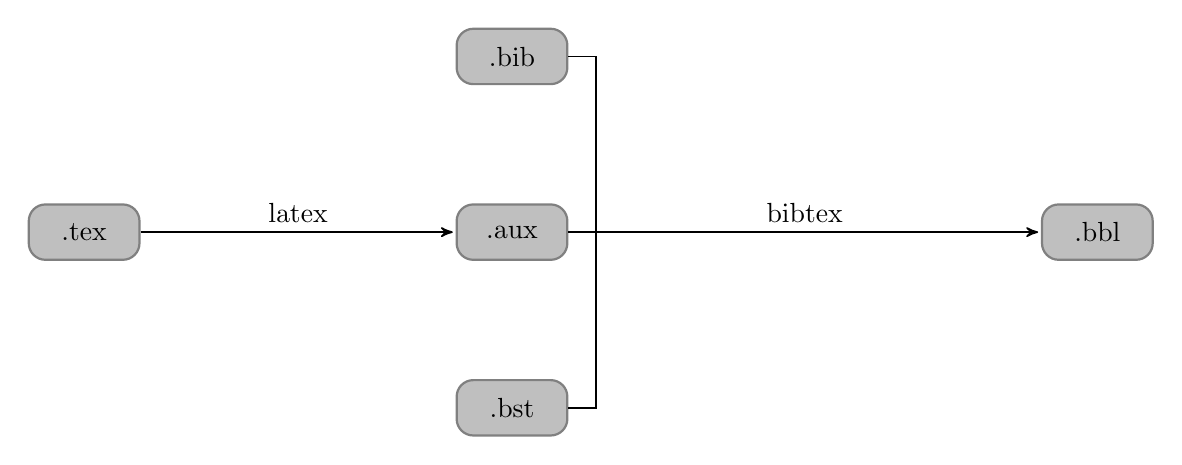
\begin{tikzpicture}
    \node[box] (tex) {.tex};
    \node[box, right=4 of tex] (aux) {.aux};
    \node[box, right=6 of aux] (bbl) {.bbl};
    \node[box, above=1.5 of aux] (bib) {.bib};
    \node[box, below=1.5 of aux] (bst) {.bst};
    \path (tex) edge [arrow] node[auto] {latex} (aux)
        (aux) edge [arrow] node[auto] {bibtex} (bbl)
        (bib.east) edge [rloop] (bst);
\end{tikzpicture}
\caption{\BibTeX~的编译}
\label{fig:bibtex}
\end{figure}

注意在长文档中使用参考文献时,应该用~\verb|latex|~编译主控文档,而用~\verb|bibtex|~编译子文档。

\begin{code}
latex master(.tex)
bibtex chapter1(.tex)
latex master(.tex)
latex master(.tex)
\end{code}

\subsection{natbib}
参考文献的引用通常有两种样式:作者-年份和数字。\LaTeX~本身只支持数字样式,而~\verb|natbib|~宏包\citep{Daly_2007}则同时支持这两种样式。

使用~\verb|natbib|~宏包时,我们首先要引用宏包;其次设置文献列表样式和引用样式,每种列表样式都有自己的缺省引用样式,所以后者可选;然后指定参考文献数据库。
\begin{code}
\usepackage{natbib}
...
\begin{document}
\bibliographystyle{plainnat}
\setcitestyle{square,aysep={},yysep={;}}
\bibliography{mybib.bib}
...
\end{document}
\end{code}

\verb|natbib|~提供了三种列表样式:plainnat、abbrvnat、unsrtnat。前两种都是作者-年份样式,文献列表按作者-年份排序,后者会使用一些缩写(比如作者的~first name);unsrtnat~是数字样式,文献列表按引用顺序排序。

\verb|\setcitestyle|~命令可以用来改变引用样式的设置,其选项见~\Fref{tab:citestyle}。

\begin{table}[htbp]
\caption{参考文献引用样式选项}
\label{tab:citestyle}
\centering
\begin{tabular}{ll}
    \toprule
    引用模式            & authoryear、numbers、super \\
    括号                & round、square、open={char},close={char} \\
    引用条目分隔符      & 分号、逗号、citesep={char} \\
    作者年份分隔符      & aysep={char} \\
    共同作者年份分隔符  & yysep={char} \\
    注解分隔符          & notesep={text} \\
    \bottomrule
\end{tabular}
\end{table}

注意在长文档中,每个含参考文献的子文档都需要分别设置列表样式,并指定数据库。

\verb|natbib|~提供了多种引用命令,其中最基本的是~\verb|\citet|~和~\verb|\citep|~,它们在不同引用模式下效果不同。一般不推荐使用~\LaTeX~本身提供的~\verb|\cite|,因为它在作者-年份模式下和~\verb|\citet|~一样,在数字模式下和~\verb|\citep|~一样。

作者-年份模式下引用命令的效果如下。
\setcitestyle{authoryear}
\begin{demo}
参阅\cite{Daly_2007}\\
参阅\citet{Daly_2007}\\
参阅\citep{Daly_2007}
\end{demo}

数字模式下引用命令的效果如下。
\setcitestyle{numbers}
\begin{demo}
参阅\cite{Daly_2007}\\
参阅\citet{Daly_2007}\\
参阅\citep{Daly_2007}
\end{demo}

上标模式下引用命令的效果如下。
\setcitestyle{super}
\begin{demo}
参阅\cite{Daly_2007}\\
参阅\citet{Daly_2007}\\
参阅\citep{Daly_2007}
\end{demo}

另外还有一些引用命令,如~\verb|\citetext、\citenum、\citeauthor|、~\verb|\citeyear|~等,此处不赘述。

\section{索引}
\verb|makeidx|~宏包提供了索引功能。应用它时,我们首先需要在文档序言部分引用宏包,并使用~\verb|makeindex|~命令;其次在正文中需要索引的地方定义索引,注意索引关键字在全文中须保持唯一;最后在合适的地方(一般是文档末尾)打印索引。

\begin{code}
\usepackage{makeidx}
\makeindex
...
\begin{document}
\index{索引关键字}
...
\printindex
\end{document}
\end{code}

当编译含索引的文档时,用户需要执行~\verb|latex、makeindex、latex|~等三次编译操作。

\begin{enumerate}
    \item 第一遍~\verb|latex|~把索引条目写到一个~\verb|.idx|~文件中去。
    \item \verb|makeindex|~把~\verb|.idx|~排序后写到一个~\verb|.ind|~文件中去。
    \item 第二遍~\verb|latex|~在~\verb|\printindex|~命令的地方引用~\verb|.ind|~的内容,生成正确的DVI。
\end{enumerate}

\begin{figure}[htbp]
\centering
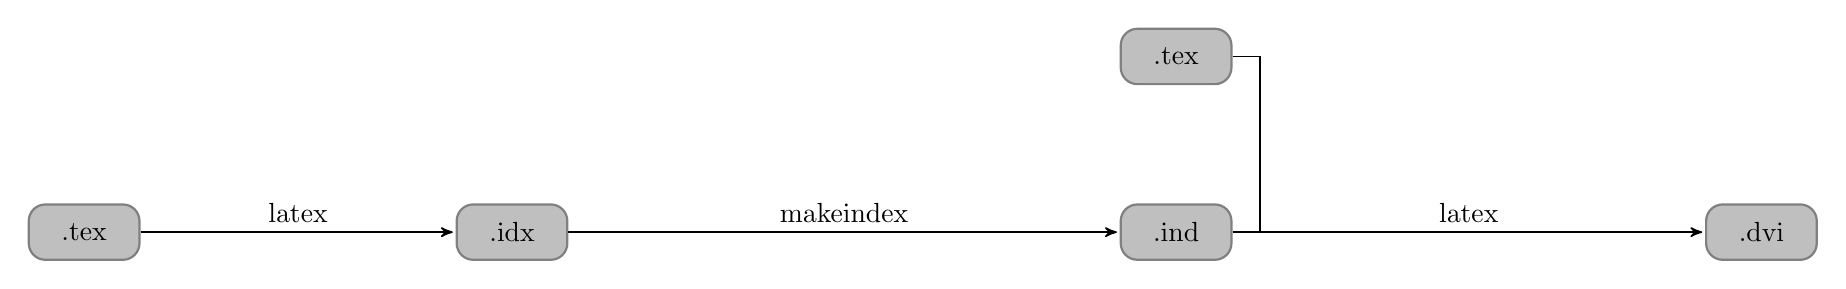
\begin{tikzpicture}
    \node[box] (tex) {.tex};
    \node[box, right=4 of tex] (idx) {.idx};
    \node[box, right=7 of idx] (ind) {.ind};
    \node[box, right=6 of ind] (dvi) {.dvi};
    \node[box, above=1.5 of ind] (tex1) {.tex};
    \node[right=1 of ind] (point) {};
    \path (tex) edge [arrow] node[auto] {latex} (idx)
        (idx) edge [arrow] node[auto] {makeindex} (ind)
        (ind) edge [arrow] node[auto] {latex} (dvi)
        (tex1.east) edge [rloop] (point);
\end{tikzpicture}
\caption{索引的编译}
\label{fig:makeidx}
\end{figure}

\section{页面布局}
在~\LaTeX~中用户可以通过~\verb|\pagestyle|~和~\verb|\pagenumbering|~命令来设置页眉(header)、页脚(footer)的样式和内容。页面样式有以下四种。

\begin{table}[htbp]
\caption{\LaTeX~页面样式}
\centering
\begin{tabular}{ll}
    \toprule
    \texttt{empty} & 页眉、页脚空白 \\
    \texttt{plain} & 页眉空白,页脚含居中页码 \\
    \texttt{headings} & 页脚空白,页眉含章节名和页码 \\
    \texttt{myheadings} & 页脚空白,页眉含页码和用户自定义信息 \\
    \bottomrule
\end{tabular}
\end{table}

\verb|fancyhdr|\citep{Oostrum_2004}宏包提供了更灵活的控制。我们可以用以下代码定制页眉、页脚的内容,以及页眉下方、页脚上方的横线。

\begin{code}
\usepackage{fancyhdr}
...
\pagestyle{fancy} %fancyhdr宏包新增的页面风格
\lhead{左擎苍}
\chead{三个代表}
\rhead{右牵黄}
\lfoot{左青龙}
\cfoot{八荣八耻}
\rfoot{右白虎}
\renewcommand{\headrulewidth}{0.4pt}
\renewcommand{\footrulewidth}{0.4pt}
\end{code}

\ \\
\begin{tikzpicture}
\draw (0,0) rectangle (36,10);
\node at(2,9) {左擎苍};
\node at(18,9) {三个代表};
\node at(34,9) {右牵黄};
\draw (.5,8)--(35.5,8);
\node at(18,5) {和谐社会};
\draw (.5,2)--(35.5,2);
\node at(2,1) {左青龙};
\node at(18,1) {八荣八耻};
\node at(34,1) {右白虎};
\end{tikzpicture}

用户可以在页眉、页脚中使用一些~\LaTeX~变量,比如分别代表页码和章节编号的~\verb|\thepage、\thechapter、\thesection|;代表章节起始单词(Chapter、Section等)的~\verb|\chaptername、\sectionname|~等。

这些变量组合起来可以构成复合标记~\verb|\leftmark|~和~\verb|\rightmark|~。当文档奇偶页面布局不同时,我们可以使用以下方法为奇偶页分别设置页眉、页脚。\verb|fancyhdr|~宏包会自动把每章起始页的样式设为~\verb|plain|,若想去掉页脚中间的页码,可以重定义~\verb|plain|~样式。

\begin{code}
\pagestyle{fancy}
\fancyhf{}                  %清空页眉页脚
\fancyhead[LE,RO]{\thepage} %偶数页左,奇数页右
\fancyhead[RE]{\leftmark}   %偶数页右
\fancyhead[LO]{\rightmark}  %奇数页左
\fancypagestyle{plain}{     %重定义plain页面样式
    \fancyhf{}
    \renewcommand{\headrulewidth}{0pt}
}
\end{code}

\ \\
\begin{tikzpicture}
\draw (0,0) rectangle (36,10);
\node at(2.5,9) {3.2 节名};
\node at(35,9) {17};
\draw (.5,8)--(35.5,8);
\node at(18,5) {奇数页};
\end{tikzpicture}

\ \\
\begin{tikzpicture}
\draw (0,0) rectangle (36,10);
\node at(1,9) {18};
\node at(32,9) {Chapter 3 章名};
\draw (.5,8)--(35.5,8);
\node at(18,5) {偶数页};
\end{tikzpicture}

Lamport当初设计~\LaTeX~时把页面布局变量的定义方式搞得比较晦涩,用户在重定义~\verb|\leftmark|~和~\verb|\rightmark|~时,不能直接用~\verb|\renewcommand|~的方法,而要用另外两个命令。

\begin{code}
\markboth{main-mark}{sub-mark}
\markright{sub-mark}
\end{code}

\verb|\leftmark|~即~main-mark,是一种高层次标记,在~article~文档类中它包含~section~的信息,在~report~和~book~则包含~chapter~的信息;\verb|rightmark|~则是一种低层次标记,在~article~中包含~subsection~信息,在~report~和~book~中包含~section~信息。

比如在~\verb|book|~文档类中,章节标记是通过下面的方法定义的,其中的~\verb|#1|~指的是章节的名字。

\begin{code}
\renewcommand\chaptermark[1]{\markboth{\chaptername \thechapter. 
    #1}{}}
\renewcommand\sectionmark[1]{\markright{\thesection. #1}}
\end{code}

%\section{演示文档}

\bibliographystyle{unsrtnat}
\bibliography{reading}
\newpage

\chapter{中文}

\section{字符集和编码}
\label{sec:encoding}

众所周知电脑内部采用二进制编码,因为它易于用电子电路实现。所有字符(包括字母、数字、符号、控制码等)在电脑内部都是用二进制表示的,字符集(Character Set)的二进制编码被称为字符编码(Character Encoding),有时人们也会混用这两个术语。

1963~年发布的~American Standard Code for Information Interchange(~ASCII)是最早出现的字符编码,它用~7~位(bit)表示了~$2^7=128$个字符,只能勉强覆盖英文字符。

美国人发明了电脑,英语被优先考虑是很自然的事情。随着电脑技术的传播,人们呼吁把字符编码扩充到~8~位也就是一个字节(byte),于是国际标准化组织(International Organization for Standardization,ISO)推出了~ISO 8859。$2^8=256$个字符显然也不能满足需要,所以~8859~被分为十几个部分,从~8859-1(西欧语言)、8859-2(中欧语言),直到~8859-16(东南欧语言),覆盖了大部分使用拉丁字母的语言文字。

在~ISO~标准完全定型之前,IBM~就有一系列自己的字符编码,他们称之为代码页(Code Page),其中著名的有~1981~年就被用于~IBM PC~的~437(扩展~ASCII)、850(西欧语言)、852(东欧语言)。IBM~代码页通常被用于控制台(Console)环境,也就是~MS-DOS~或~Unix Shell~那样的命令行环境。

微软将~IBM~代码页称为~OEM~代码页,自己定义的称为~ANSI~代码页,后者中著名的有1252(西欧语言)、1250(东欧语言)、936(GBK~简体中文)、950(Big5~繁体中文)、932(SJIS~日文)、949(EUC-KR~韩文)等。

1981~年,中国大陆推出了第一个自己的字符集标准~GB2312,它是一个~$94*94$~的表,包括~7445~个字符(含~6763~个汉字)。GB2312~通常采用双字节的EUC-CN编码,所以后者也常常被称为~GB2312~编码;其实~GB2312~还有另一种编码方式~HZ,只是不常用。GB2312~不包含朱镕基的“镕”字,政府、新闻、出版、印刷等行业和部门在使用中感到十分不便,于是它在~1993~年被扩展为~GBK,后者包括~21886~个字符(含~21003~个汉字),没有形成正式标准。2000~年发布的~GB18030~包含~70244~个字符(含~27533~个汉字),采用四字节编码。GB18030~之前还出现过一个~GB13000,没有形成气候。

1990~年ISO~推出了通用字符集(Universal Character Set,UCS),即~ISO 10646,意图一统江湖。它有两种编码:双字节的~UCS-2~和四字节的~UCS-4。

ISO~之外还有个希望一统江湖的组织:统一码联盟(The Unicode Consortium),它于~1991~年推出了~Unicode 1.0。后来两家组织意识到没必要做重复工作,于是开始合并双方的成果,携手奔小康。从~Unicode 2.0~开始,Unicode~采用了与~ISO 10646-1~相同的编码。

Unicode~主要有三种编码:UTF-8、UTF-16、UTF-32。UTF-8~使用一至四个~8~位编码。互联网工程任务组(Internet Engineering Task Force,~IETF)要求所有网络协议都支持~UTF-8,互联网电子邮件联盟(Internet Mail Consortium,IMC)也建议所有电子邮件软件都支持~UTF-8,所以它已成为互联网上的事实标准。UTF-16~用一或两个~16~位编码,基本上是~UCS-2~的超集,和~ASCII~不兼容。UTF-32~用一个~32~位编码,它是~UCS-4~的一个子集。

\section{中文解决方案}
\TeX~是基于单字节编码的,因为~Knuth~当初开发~\TeX~时没考虑那么远,也没有现成的标准可以借鉴。

\LaTeX~对中文的支持主要有两种方法:张林波\footnote{中科院计算数学所某实验室主任。}开发的~\href{ftp://ftp.cc.ac.cn/pub/cct/}{CCT}~和~Werner Lemberg\footnote{1968~年生于奥地利,从维也纳音乐学院获得作曲、指挥、钢琴、乐团管理、歌手教练等五个专业文凭,后自学中文和数学。曾任职于奥地利和德国多家剧院和乐团,现任德国科布伦茨某剧院指挥。}开发的~CJK~宏包。早期~CCT~比较流行,新的~CCT~也可以和~CJK~配合使用,网上可以找到的最后更新是~2003~年的。CJK~是当前主流,它不仅支持中日韩等东亚文字,还支持几十种其他不同语言的多种编码。

支持简体中文的~\LaTeX~发行版有吴凌云\footnote{中科院应用数学所研究员。}的~CTeX~和李树钧\footnote{德国哈根函授大学研究员。}的~ChinaTeX,繁体中文的有吴聪敏\footnote{台湾大学电机系学士,美国罗彻斯特大学经济学博士,现任台湾大学经济系教授。}、吴聪慧兄弟的~cwTeX~和蔡奇伟\footnote{美国犹他大学计算机博士,现任台湾静宜大学资讯工程系教授。}的~PUTeX。后面两个台湾的发行版包老师不熟悉,前面两个大陆的发行版都包含~MikTeX、CCT、CJK、WinEdt~等。

\section{CJK的使用}
CJK~的作者写的使用说明比较凌乱和晦涩,读者可以参阅李果正的《我的CJK》\citep{Lee_2004a}。

CJK~有两个基本宏包:\verb|CJK|~和~\verb|CJKutf8|,后者面向~UTF-8~编码。CJK~环境的一般使用方法如下:

\begin{code}
\usepackage{CJK(utf8)}
...
\begin{document}
\begin{CJK}{<encoding>}{<family>}
...
\end{CJK}
\end{document}
\end{code}

简体中文常用编码是~GBK~和~UTF8~。family~是指宋体、楷体、隶书等,具体引用要看电脑上安装了什么字体。麻烦的是~GBK~和~UTF8~字体不通用,也就是说每种编码需要自己的字体。CJK~自带的~UTF8~简体字体有~gbsn(宋体)和~gkai(楷体)。CTeX~提供的~GBK~字体有~song(宋体)、fs(仿宋)、kai(楷体)、hei(黑体)、li(隶书)、~you(幼圆)等。

注意使用~\verb|CJKutf8|~宏包时,\verb|CJK|~环境的编码最好是~UTF8,否则可能遭遇不测。

下面是一个简单的~GBK~示例和一个~UTF8~示例,注意用编辑器保存时要选则相应的编码格式,比如前者用~ANSI,后者用~UTF-8。
\begin{code}
\documentclass{article}
\usepackage{CJK}
\begin{document}
\begin{CJK}{GBK}{song}
这是一个CJK例子,使用了GBK编码和song字体。
\end{CJK}
\end{document}
\end{code}

\begin{code}
\documentclass{article}
\usepackage{CJKutf8}
\begin{document}
\begin{CJK}{UTF8}{gbsn}
这是一个CJK例子,使用了UTF-8编码和gbsn字体。
\end{CJK}
\end{document}
\end{code}

\bibliographystyle{unsrtnat}
\bibliography{reading}
\newpage

% This is part of the book TeX for the Impatient.
% Copyright (C) 2003 Paul W. Abrahams, Kathryn A. Hargreaves, Karl Berry.
% See file fdl.tex for copying conditions.

% Fonts for TeX for the Impatient.

% This file is being distributed with the macros because the macro file
% refers to it.  We used a combination of Bitstream and standard TeX
% fonts for the original printed book, but for the free edition, we
% stick to Computer Modern.
% -----------------------------------------------------------------------
% 
% We used Computer Modern for the main text and math, and Zapf Humanist
% (i.e., Optima) for heads.  (bs00015 is Optima Roman, 16 italic, 17
% bold, 18 bold italic.)  
% 
% First we define all of the fonts we use for any purpose, in terms of the
% font files.  Later we define fonts functionally, using \let or \def.

% Computer Modern fonts.
%
\ifadobefont
  \def\song{Adobe Song Std}
  \def\hei{Adobe Heiti Std}
  \def\kai{Adobe Kaiti Std}
  \def\fang{Adobe Fangsong Std}
\else
  \def\song{SimSun}
  \def\hei{SimHei}
  \def\kai{KaiTi}
  \def\fang{FangSong}
\fi
%
\ifxecjk
  \font\CJKfont="\song" at 10pt
  \input xeCJK-base
  \def\letfont{\let\CJKfont}
  \normalspacedchars{-}
\else
  \font\zhfont="\song" at 10pt
  \def\zhpunctfont{\zhfont}
  \input zhspacing.sty
  \zhspacing
  \def\letfont{\let\zhfont}
\fi
%
\font\enfiverm = cmr5
\font\zhfiverm = "\song" at 5pt
\def\fiverm{\enfiverm\letfont\zhfiverm}
\font\eneightrm = cmr8
\font\zheightrm = "\song" at 8pt
\def\eightrm{\eneightrm\letfont\zheightrm}
\font\enninerm = cmr9 % Glue pictures, small caps for ASCII.
\font\zhninerm = "\song" at 9pt
\def\ninerm{\enninerm\letfont\zhninerm}
%\font\tenrm = xcmr10 % with our kerning
\font\entenrm = cmr10 % don't have the xcmr10 source any more
\font\zhtenrm = "\song"  at 10pt
\def\tenrm{\entenrm\letfont\zhtenrm}
\font\enoldtenrm = cmr10 % straight CM
\font\zholdtenrm = "\song"  at 10pt
\def\oldtenrm{\enoldtenrm\letfont\zholdtenrm}
\font\entwelverm = cmr12
\font\zhtwelverm = "\song"  at 12pt
\def\twelverm{\entwelverm\letfont\zhtwelverm}
\font\entwentysixrm = cmr10 at 26pt
\font\zhtwentysixrm = "\hei"  at 26pt
\def\twentysixrm{\entwentysixrm\letfont\zhtwentysixrm}
%
\font\eneightit = cmti8
\font\zheightit = "\kai" at 8pt
\def\eightit{\eneightit\letfont\zheightit}
\font\ennineit = cmti9
\font\zheightit = "\kai" at 9pt
\def\nineit{\ennineit\letfont\zhnineit}
\font\entenit = cmti10
\font\zhtenit = "\kai" at 10pt
\def\tenit{\entenit\letfont\zhtenit}
%
\font\eneighttt = cmtt8
\font\zheighttt = "\fang" at 8pt
\def\eighttt{\eneighttt\letfont\zheighttt}
\font\ententt = cmtt10
\font\zhtentt = "\fang" at 10pt
\def\tentt{\ententt\letfont\zhtentt}
\font\eneleventt = cmtt10 at 11pt
\font\zheleventt = "\fang" at 11pt
\def\elventt{\enelventt\letfont\zhelventt}
\font\entwelvett = cmtt10 scaled \magstep2
\font\zhtwelvett = "\fang" at 12pt
\def\twelvett{\entwelvett\letfont\zhtwelvett}
%
\font\entenbt = cmtt10
\font\zhtenbt = "\fang" at 10pt
\def\tenbt{\entenbt\letfont\zhtenbt}
%
\font\enelevensf = cmss10 scaled\magstephalf
\font\zhelevensf = "\hei" at 11pt
\def\elevensf{\enelevensf\letfont\zhelevensf}
\font\enfourteensf = cmss10 scaled\magstep2
\font\zhfourteensf = "\hei" at 14pt
\def\fourteensf{\enfourteensf\letfont\zhfourteensf}
%
\font\eneightbf = cmbx8
\font\zheightbf = "\hei" at 8pt
\def\eightbf{\eneightbf\letfont\zheightbf}
\font\entenbf = cmbx10
\font\zhtenbf = "\hei" at 10pt
\def\tenbf{\entenbf\letfont\zhtenbf}
\font\enelevenbf = cmbx10 scaled \magstephalf
\font\zhelevenbf = "\hei" at 11pt
\def\elevenbf{\enelevenbf\letfont\zhelevenbf}
\font\entwelvebf = cmbx12
\font\zhtwelvebf = "\hei" at 12pt
\def\twelvebf{\entwelvebf\letfont\zhtwelvebf}
\font\enthirtysixbf = cmbx10 at 36pt
\font\zhthirtysixbf = "\hei" at 36pt
\def\thirtysixbf{\enthirtysixbf\letfont\zhthirtysixbf}
%
\font\entenbi = cmbxti10
\font\zhtenbi = "\hei" at 10pt
\def\tenbi{\entenbi\letfont\zhtenbi}
\font\enelevenbi= cmbxti10 scaled \magstephalf
\font\zhelevenbi = "\hei" at 11pt
\def\elevenbi{\enelevenbi\letfont\zhelevenbi}
\font\enfourteenbi= cmbxti10 scaled \magstep2
\font\zhfourteenbi = "\hei" at 14pt
\def\fourteenbi{\enfourteenbi\letfont\zhfourteenbi}
%
\font\entensc = cmcsc10
\font\zhtensc = "\fang" at 10pt
\def\tensc{\entensc\letfont\zhtensc}
\font\eneightsl = cmsl8
\font\zheightsl = "\fang" at 8pt
\def\eightsl{\eneightsl\letfont\zheightsl}
\font\eneighti = cmmi8
\font\zheighti = "\kai" at 8pt
\def\eighti{\eneighti\letfont\zheighti}
\font\eneightsy = cmsy8
\font\zheightsy = "\song" at 8pt
\def\eightsy{\eneightsy\letfont\zheightsy}

% % Optima fonts.
% %
% \font\eightopt = bs0015 at 8pt
% \font\nineopt = bs0015 at 9pt
% \font\twelveopt = bs0015 at 12pt
% \font\twentysixopt = bs0015 at 26pt
% \font\nineoptit = bs0016 at 9pt
% \font\tenoptit = bs0016 at 10pt
% \font\tenoptbf = bs0017 at 10pt
% \font\thirtysixoptbf = bs0017 at 36pt
% \font\tenbt = bs00175 at 10pt
% \font\tenoptbi = bs0018 at 10pt
% \font\elevenoptbi = bs0018 at 11pt
% \font\fourteenoptbi = bs0018 at 14pt
 
% Palatino fonts.
%
\font\tenpal = pplr
%\font\tenpal = bs0023
%\font\tenpalit = bs0024
%\font\tenpalbf = bs0025
%\font\tenpalbi = bs0026

% Logo and picture fonts.
% 
\font\eightlogo = logo8
\font\logosl = logosl10
\font\handfont = pzdr

% The following changes are to avoid driver overflow
\ifmsdos
   \font\cnum = cnum % 36-pt bold Optima, numbers only (just for MS-DOS)
   \let\chapternumeralfont = \cnum
   %\let\thirtysixoptbf = \twentysixopt
   %\font\sevensy = cmsy8
   %\font\seveni = cmmi8
\fi

\def\undefinedfont{\errmessage{Undefined font}}

% This should only be called when \rm et al. are going to be defined
% directly.
% 
\def\clearfonts{\let\rm = \undefinedfont \let\bf = \undefinedfont
   \let\it = \undefinedfont \let\bi = \undefinedfont
   \let\tt = \undefinedfont \let\bt = \undefinedfont
   \let\sc = \undefinedfont
   \let\ss = \undefinedfont
}

% We only need to assign to \fam if the font is going to be used in math
% mode, which isn't the case with any of these.  \rm, \it, \sl, \bf, and
% \tt are defined in plain.
% 
\def\bi{\tenbi}

\def\mapquotes{\catcode`` = \active \catcode`' = \active}
{\mapquotes
  \gdef\bt{% The font change also draws \ ` ' from a different font.
     \tenbt
     \def\\{{\tentt \char92}}%
     \def`{{\tentt \char96}}\def'{{\tentt \char39}}%
  }
}

\def\bti{\tenbi}
\def\sc{\tensc}

% Text fonts.
% 
\def\textfonts{%
  \def\rm{\fam0\tenrm}%
  \textfont0=\tenrm \scriptfont0=\sevenrm \scriptscriptfont0=\fiverm
  \textfont1=\teni \scriptfont1=\seveni \scriptscriptfont1=\fivei
  \textfont2=\tensy \scriptfont2=\sevensy \scriptscriptfont2=\fivesy
  \textfont3=\tenex \scriptfont3=\tenex \scriptscriptfont3=\tenex
  \def\it{\fam\itfam\tenit}\textfont\itfam=\tenit
  \def\sl{\fam\slfam\tensl}\textfont\slfam=\tensl
  \def\bf{\fam\bffam\tenbf}\textfont\bffam=\tenbf
  \scriptfont\bffam=\sevenbf \scriptscriptfont\bffam=\fivebf
  \def\tt{\fam\ttfam\tentt}\textfont\ttfam=\tentt
  \let\sc = \tensc
  \setbox\strutbox=\hbox{\vrule height8.5pt depth3.5pt width\z@}%
  \normalbaselineskip=12pt
  \normalbaselines \rm
}


% Footnote fonts.  We generally use eight point.
% 
\def\footnotefonts{%
  \def\rm{\fam0\eightrm}%
  \textfont0=\eightrm \scriptfont0=\sevenrm \scriptscriptfont0=\fiverm
  \textfont1=\eighti \scriptfont1=\seveni \scriptscriptfont1=\fivei
  \textfont2=\eightsy \scriptfont2=\sevensy \scriptscriptfont2=\fivesy
  \textfont3=\tenex \scriptfont3=\tenex \scriptscriptfont3=\tenex
  \def\it{\fam\itfam\eightit}\textfont\itfam=\eightit
  \def\sl{\fam\slfam\eightsl}\textfont\slfam=\eightsl
  \def\bf{\fam\bffam\eightbf}\textfont\bffam=\eightbf
  \scriptfont\bffam=\sevenbf \scriptscriptfont\bffam=\fivebf
  \def\tt{\fam\ttfam\eighttt}\textfont\ttfam=\eighttt
  \let\sc = \eightsc
  \setbox\strutbox=\hbox{\vrule height7pt depth2pt width\z@}%
  \normalbaselineskip=9pt
  \normalbaselines \rm
}

% Fonts for the example titles.  They are defined in the first example,
% also.
% 

\def\exampletitlefonts{\clearfonts 
   \let\bf = \elevenbf
   \let\bi = \elevenbi
   \baselineskip = 13pt \bf
}

% Fonts for the subsection titles.
% 
\def\subsectionfonts{\clearfonts \let\sf = \elevensf
   \baselineskip = 12pt \sf
}


% Fonts for the section titles.
% 
\def\sectionfonts{\clearfonts \let\sf = \fourteensf
   \baselineskip = 16pt \sf
}

% Fonts for the chapter titles.
% 
\let\chapternumeralfont = \thirtysixbf

\def\chapterfonts{\clearfonts \let\bf = \twentysixrm
   \baselineskip = 32pt \bf
}

% Fonts for the table of contents.
% 
\def\shorttocfonts{\clearfonts \let\rm = \twelverm
   \baselineskip = 20pt \rm
}

\def\tocfonts{\clearfonts \let\rm = \ninerm
   \let\it = \tenit \let\bf = \tenbf
   \baselineskip = 12pt \rm
}

% Fonts for the index.
% 

\def\indexfonts{\clearfonts
   \let\rm = \eightrm
   \let\it = \eightit
   \let\tt = \eighttt
   \let\sc = \tensc
   \let\sl = \eightsl
   \textfont2 = \eightsy % For \AMSTeX.
   \let\mflogo = \eightlogo % For \Metafont.
   \normalbaselineskip = 10pt \normallineskip = 1.5pt \normalbaselines
   \setbox\strutbox=\hbox{\vrule height 7.5pt depth2.5pt width0pt}%
   \rm
}

% Fonts for the inside back cover.
% 
\def\conceptpagefonts{\clearfonts
   \let\rm = \ninerm
   \let\sc = \eightrm
   \let\sl = \nineit
   \baselineskip = 12pt
   \rm
}

% We don't want any automatic hyphenation within the code font

\hyphenchar\zhtentt = -1
\hyphenchar\ententt = -1
\hyphenchar\zheighttt = -1
\hyphenchar\eneighttt = -1



\textfonts


\backmatter
\chapter{跋}

首先向一路披荆斩棘看到这里的读者表示祝贺,至少在精神上你已经成为一名合格的~\LaTeX{}er。从此你生是~\LaTeX~的人,死是~\LaTeX~的鬼。Once Black, never back。没有坚持到这里的同学自然已经重新投向“邪恶”的~MS Word,毕竟那里点个按钮就可以插入图形,点个下拉框就可以选择字体。

当然~\LaTeX{}er也有简单的出路,就是只使用缺省设置,尽量少用插图;不必理会点阵、矢量,也不必理会~Type 1、Type 3、TrueType、OpenType。因为内容高于形式,你把文章的版面、字体搞得再漂亮,它也不会因此成为《红楼梦》;而《红楼梦》即使是手抄本,也依然是不朽的名著。

包老师曾经以为~\LaTeX~和~Word~的关系就好像是《笑傲江湖》中华山的气宗和剑宗,头十年剑宗进步快,中间十年打个平手,再往后气宗就遥遥领先。至于令狐冲的无招胜有招,风清扬的神龙见首不见尾又是另一重境界,普通人恐怕只能望其颈背。

费尽九牛二虎之力熬到本文杀青的时候,才发现从前的想法很傻很天真。让我们挥一挥衣袖,不带走一片云,卧薪尝胆忍辱负重,耐心等待~\XeTeX~和~Lua\TeX。

%chapter*{索引}
%\printindex

\newpage

\end{CJK*}

\end{document}